\documentclass{Configuration_Files/PoliMi3i_thesis}

%------------------------------------------------------------------------------
%	REQUIRED PACKAGES AND  CONFIGURATIONS
%------------------------------------------------------------------------------

% CONFIGURATIONS
\usepackage{parskip} % For paragraph layout
\usepackage{setspace} % For using single or double spacing
\usepackage{emptypage} % To insert empty pages
\usepackage{multicol} % To write in multiple columns (executive summary)
\setlength\columnsep{15pt} % Column separation in executive summary
\setlength\parindent{0pt} % Indentation
\raggedbottom  

% PACKAGES FOR TITLES
\usepackage{titlesec}
% \titlespacing{\section}{left spacing}{before spacing}{after spacing}
\titlespacing{\section}{0pt}{3.3ex}{2ex}
\titlespacing{\subsection}{0pt}{3.3ex}{1.65ex}
\titlespacing{\subsubsection}{0pt}{3.3ex}{1ex}
\usepackage{color}

% PACKAGES FOR LANGUAGE AND FONT
\usepackage[english]{babel} % The document is in English  
\usepackage[utf8]{inputenc} % UTF8 encoding
\usepackage[T1]{fontenc} % Font encoding
\usepackage[11pt]{moresize} % Big fonts

% PACKAGES FOR IMAGES
\usepackage{graphicx}
\usepackage{transparent} % Enables transparent images
\usepackage{eso-pic} % For the background picture on the title page
\usepackage{subfig} % Numbered and caption subfigures using \subfloat.
\usepackage{tikz} % A package for high-quality hand-made figures.
\usetikzlibrary{}
\graphicspath{{./Images/}} % Directory of the images
\usepackage{caption} % Coloured captions
\usepackage{xcolor} % Coloured captions
\usepackage{amsthm,thmtools,xcolor} % Coloured "Theorem"
\usepackage{float}  

% STANDARD MATH PACKAGES
\usepackage{amsmath}
\usepackage{amsthm}
\usepackage{amssymb}
\usepackage{amsfonts}
\usepackage{bm}
\usepackage[overload]{empheq} % For braced-style systems of equations.
\usepackage{fix-cm} % To override original LaTeX restrictions on sizes

% PACKAGES FOR TABLES
\usepackage{tabularx}
\usepackage{longtable} % Tables that can span several pages
\usepackage{colortbl}
\usepackage{array}
\usepackage{hhline}
% PACKAGES FOR ALGORITHMS (PSEUDO-CODE)
\usepackage{algorithm}
\usepackage{algorithmic}

% PACKAGES FOR REFERENCES & BIBLIOGRAPHY
\usepackage[colorlinks=true,linkcolor=black,anchorcolor=black,citecolor=black,filecolor=black,menucolor=black,runcolor=black,urlcolor=black]{hyperref} % Adds clickable links at references
\usepackage{cleveref}
\usepackage[square, numbers, sort&compress]{natbib} % Square brackets, citing references with numbers, citations sorted by appearance in the text and compressed
\bibliographystyle{abbrvnat} % You may use a different style adapted to your field

% OTHER PACKAGES
\usepackage{pdfpages} % To include a pdf file
\usepackage{afterpage}
\usepackage{lipsum} % DUMMY PACKAGE
\usepackage{fancyhdr} % For the headers
\fancyhf{}
\usepackage{comment}
\usepackage{enumitem}
\usepackage{xurl}
% Input of configuration file. Do not change config.tex file unless you really know what you are doing. 
% Define blue color typical of polimi
\definecolor{bluepoli}{cmyk}{0.4,0.1,0,0.4}

% Custom theorem environments
\declaretheoremstyle[
  headfont=\color{bluepoli}\normalfont\bfseries,
  bodyfont=\color{black}\normalfont\itshape,
]{colored}

% Set-up caption colors
\captionsetup[figure]{labelfont={color=bluepoli}} % Set colour of the captions
\captionsetup[table]{labelfont={color=bluepoli}} % Set colour of the captions
\captionsetup[algorithm]{labelfont={color=bluepoli}} % Set colour of the captions

\theoremstyle{colored}
\newtheorem{theorem}{Theorem}[chapter]
\newtheorem{proposition}{Proposition}[chapter]

% Enhances the features of the standard "table" and "tabular" environments.
\newcommand\T{\rule{0pt}{2.6ex}}
\newcommand\B{\rule[-1.2ex]{0pt}{0pt}}

% Pseudo-code algorithm descriptions.
\newcounter{algsubstate}
\renewcommand{\thealgsubstate}{\alph{algsubstate}}
\newenvironment{algsubstates}
  {\setcounter{algsubstate}{0}%
   \renewcommand{\STATE}{%
     \stepcounter{algsubstate}%
     \Statex {\small\thealgsubstate:}\space}}
  {}

% New font size
\newcommand\numfontsize{\@setfontsize\Huge{200}{60}}

% Title format: chapter
\titleformat{\chapter}[hang]{
\fontsize{50}{20}\selectfont\bfseries\filright}{\textcolor{bluepoli} \thechapter\hsp\hspace{2mm}\textcolor{bluepoli}{|   }\hsp}{0pt}{\huge\bfseries \textcolor{bluepoli}
}

% Title format: section
\titleformat{\section}
{\color{bluepoli}\normalfont\Large\bfseries}
{\color{bluepoli}\thesection.}{1em}{}

% Title format: subsection
\titleformat{\subsection}
{\color{bluepoli}\normalfont\large\bfseries}
{\color{bluepoli}\thesubsection.}{1em}{}

% Title format: subsubsection
\titleformat{\subsubsection}
{\color{bluepoli}\normalfont\large\bfseries}
{\color{bluepoli}\thesubsubsection.}{1em}{}

% Shortening for setting no horizontal-spacing
\newcommand{\hsp}{\hspace{0pt}}

\makeatletter
% Renewcommand: cleardoublepage including the background pic
\renewcommand*\cleardoublepage{%
  \clearpage\if@twoside\ifodd\c@page\else
  \null
  \AddToShipoutPicture*{\BackgroundPic}
  \thispagestyle{empty}%
  \newpage
  \if@twocolumn\hbox{}\newpage\fi\fi\fi}
\makeatother

%For correctly numbering algorithms
\numberwithin{algorithm}{chapter}

%----------------------------------------------------------------------------
%	NEW COMMANDS DEFINED
%----------------------------------------------------------------------------

% EXAMPLES OF NEW COMMANDS
\newcommand{\bea}{\begin{eqnarray}} % Shortcut for equation arrays
\newcommand{\eea}{\end{eqnarray}}
\newcommand{\e}[1]{\times 10^{#1}}  % Powers of 10 notation

\newcolumntype{P}[1]{>{\centering\arraybackslash}p{#1}}

%----------------------------------------------------------------------------
%	ADD YOUR PACKAGES (be careful of package interaction)
%----------------------------------------------------------------------------

%----------------------------------------------------------------------------
%	ADD YOUR DEFINITIONS AND COMMANDS (be careful of existing commands)
%----------------------------------------------------------------------------

%----------------------------------------------------------------------------
%	BEGIN OF YOUR DOCUMENT
%----------------------------------------------------------------------------

\begin{document}

%\fancypagestyle{plain}{%
%\fancyhf{} % Clear all header and footer fields
%\fancyhead[RO,RE]{\thepage} %RO=right odd, RE=right even
%\renewcommand{\headrulewidth}{0pt}
%\renewcommand{\footrulewidth}{0pt}}

%----------------------------------------------------------------------------
%	TITLE PAGE
%----------------------------------------------------------------------------

\pagestyle{plain} % No page numbers
\frontmatter % Use roman page numbering style (i, ii, iii, iv...) for the preamble pages

\puttitle{
	title=eMall – e-Mobility for All, % Title of the thesis
	name=\\Andrea Piras - 10725972\\Emanuele Santoro - 10676582\\Andrea Sanguineti - 10739788, % Author Name and Surname
	course=Software Engineering 2, % Study Programme (in Italian)
	academicyear={2022-23},  % Academic Year
} % These info will be put into your Title page 

%----------------------------------------------------------------------------
%	PREAMBLE PAGES: ABSTRACT (inglese e italiano), EXECUTIVE SUMMARY
%----------------------------------------------------------------------------
\setcounter{page}{1} % Set page counter to 1



%----------------------------------------------------------------------------
%	LIST OF CONTENTS/FIGURES/TABLES/SYMBOLS
%----------------------------------------------------------------------------

% TABLE OF CONTENTS
\thispagestyle{empty}
\tableofcontents % Table of contents 
\thispagestyle{empty}

%-------------------------------------------------------------------------
%	THESIS MAIN TEXT
%-------------------------------------------------------------------------
% In the main text of your thesis you can write the chapters in two different ways:
%
%(1) As presented in this template you can write:
%    \chapter{Title of the chapter}
%    *body of the chapter*
%
%(2) You can write your chapter in a separated .tex file and then include it in the main file with the following command:
%    \chapter{Title of the chapter}
%    \input{chapter_file.tex}
%
% Especially for long thesis, we recommend you the second option.

\addtocontents{toc}{\vspace{2em}} % Add a gap in the Contents, for aesthetics
\mainmatter % Begin numeric (1,2,3...) page numbering

% --------------------------------------------------------------------------
% NUMBERED CHAPTERS % Regular chapters following
% --------------------------------------------------------------------------
\onehalfspacing
\newcounter{row}
\newcommand\row{\stepcounter{row}\arabic{row}}
\chapter{INTRODUCTION}
\label{ch:introduction}%
% The \label{...}% enables to remove the small indentation that is generated, always leave the % symbol.

\section{Purpose}
Electric vehicles are the key technology to reduce the environmental impact of road transport, a sector that accounts for 16\% of global emissions. Recent years have seen exponential growth in the sale of electric vehicles together with improved range, wider model availability and increased performance. \\ \\
This trend is projected to continue in the future, and for this reason more charging stations are being built each year, in order to satisfy the increasing demand for energy for these electric vehicles. \\ \\
In this context, it is fundamental that the communication between the charging stations and the drivers is managed in such a way that it introduces minimal interference and constraints on 
our daily schedule. \\ \\
eMall is going to be a platform that permits the aforementioned communication through its subsystems eMSP (e-Mobility Service Provider), which is the app used by some users, like drivers, and the CPMS (Charge Point Management System), used by the owner of the charging stations or also called Charging Point Operator (CPO). \\ \\
Our main goal is to develop both subsystems and in particular, describe how the eMSPs can communicate with different CPMSs. Through an eMSP, drivers can easily choose where to charge their vehicles and easily book the charging process and pay for it. On the other hand, CPOs can use their CPMS to manage their charging stations, in order to improve and speed up the energy management and the charging process.
\label{sec:purpose}
\subsection{Goals} %AP
\label{subsec:goals}
\begin{table}[H]

\centering 
    \begin{tabular}{| p{0.15\linewidth} | p{0.85\linewidth} |}
    \hline
    \rowcolor{bluepoli!40}
     \textbf{ID} & \textbf{Description} \T\B \\
    \hline \hline
    \textbf{G\row} & Allow Drivers to check nearby charging stations and see info about their prices, special offers and availability.\T\B\\
    \hline
    \textbf{G\row} & Allow Drivers to create and delete bookings for charging their vehicle in a charging station. \T\B\\
    \hline
    \textbf{G\row} & Allow Drivers to manage and monitor their charging process.\T\B\\
    \hline
    \textbf{G\row} & Allow Drivers to pay CPOs for the charging process provided.\T\B\\
    \hline
    \textbf{G\row} & Proactively suggest to the Drivers where to go to charge their vehicle.\T\B\\
    \hline
    \textbf{G\row} & Allow CPOs to manage the charging prices and the criteria of energy acquisition in their charging stations.\T\B\\
    \hline
    %\textbf{G\row} & Allow CPOs to dynamically decide how to acquire energy and how to distribute it in the charging station.\T\B\\
    %\hline
    \textbf{G\row} & Allow CPOs to connect to all their charging stations and monitor them.\T\B\\
    \hline
    \end{tabular}
    \\[10pt]
    \caption{Goals}
    \setcounter{row}{0}
\end{table}

\section{Scope}
\label{sec:scope}
The eMall platform objective is the integration between two subsystems: the eMSP and the CPMS. \\
Even though the eMSPs could be handled directly by third-party providers, in this project both subsystems are managed by eMall. \\ 
In this project, only the subsystems are described, since eMall is considered an already implemented service accessible via web and therefore only mentioned if the actors or the subsystems interact with it.
Among the several stakeholders to consider, this document concerns only drivers and CPOs. Occasionally DSOs (Distribution System Operators) are mentioned, but they should not be considered part of the project scope since they do not use the platform and are therefore external entities. \\


\subsection{World Phenomena} %AS
\label{subsec:worldPhenomena}
\begin{table}[H]
\centering 
    \begin{tabular}{| p{0.15\linewidth} | p{0.8\linewidth} |}
    \hline
    \rowcolor{bluepoli!40}
     \textbf{ID} & \textbf{Description} \T\B \\
    \hline \hline
    \textbf{WP\row} & The driver wants to charge his vehicle.\T\B\\
    \hline
    \textbf{WP\row} & The driver drives the vehicle to the booked charging socket.\T\B\\
    \hline
    \textbf{WP\row} & The CPO wants to connect one of his charging stations.\T\B\\
    \hline
    \textbf{WP\row} & The CPO decides to start using a new eMSP.\T\B\\
    \hline
    \textbf{WP\row} & A DSO updates its energy price.\T\B\\
    \hline
    \end{tabular}
    \\[10pt]
    \caption{World Phenomena}
    \setcounter{row}{0}
\end{table}

\subsection{Shared Phenomena} %ES
\label{subsec:sharedPhenomena}
\begin{longtable}{| p{0.15\linewidth} | p{0.5\linewidth} |P{0.1\linewidth} | P{0.1\linewidth}|}
    \hline
    \rowcolor{bluepoli!40}
     \textbf{ID} & \textbf{Description} & \textbf{W. C.} &\textbf{M. C.} \\
    \hline \hline
    
    \textbf{SP\row} & The Driver inserts his personal data and a payment method in order to register himself on the platform&\textbf{X} & \T\B\\
    \hline
    \textbf{SP\row}& The Driver creates a physical connection between the system and his vehicle. &\textbf{X} & \T\B\\
    \hline
    \textbf{SP\row} & The Driver receives a suggestion when he needs to charge the vehicle. & & \textbf{X}\T\B\\
    \hline
    \textbf{SP\row} & The energy level of the battery vehicle changes. & \textbf{X} & \T\B\\
    \hline
    \textbf{SP\row} & The Driver follows a new navigation route on his vehicle. & \textbf{X} & \T\B\\
    \hline
    
    %\textbf{SP\row} & The CPO check the DSOs energy prices
    %&  \textbf{X}  & \\
    %\hline
    \textbf{SP\row} & The Driver checks information about the availability and locations of nearby charging stations 
    & \textbf{X} &\\
    \hline
    \textbf{SP\row} & The Driver books a charge in a charging station.  & \textbf{X} &\T\B\\
    \hline
    \textbf{SP\row} & The Driver receives a notification that the booking process was successful & &\textbf{X}  \T\B\\
    \hline
    \textbf{SP\row} & The Driver receives a notification that the booking was successfully cancelled & &\textbf{X}  \T\B\\
    \hline
    \textbf{SP\row} & The Driver plugs his vehicle in the charging socket  &\textbf{X}& \T\B\\
    \hline
    \textbf{SP\row} & The Driver gets notified when trying to start a charging process even though his vehicle is not well-connected & &\textbf{X} \T\B\\
    \hline
    \textbf{SP\row} & The Driver receives a notification when the charging process is complete. & & \textbf{X}\T\B\\
    \hline
    \textbf{SP\row} & The CPO checks the internal status of one of the managed charging stations 
    & \textbf{X} & \\
    \hline
    \textbf{SP\row} & The CPO sets a special offer. & \textbf{X} &\T\B\\
    \hline
    \textbf{SP\row} & The CPO changes energy acquisition criteria for a charging station 
    & \textbf{X} & \\
    \hline
    \textbf{SP\row} & The CPO changes energy revenue criteria for a charging station 
    & \textbf{X} & \\
    \hline
    \textbf{SP\row} & In a charging station a socket becomes available after a charging process is finished &  \textbf{X}& \T\B\\
    \hline
    \caption{Shared Phenomena}
    \setcounter{row}{0}
\end{longtable}
\newpage
\section{Definitions, Acronyms, Abbreviations}
\label{sec:definitionsAcronymsAbbreviations}
\subsection{Definitions} %AP
\label{subsec:definitions}
\begin{table}[H]
\centering 
    \begin{tabular}{| p{0.125\linewidth} | p{0.80\linewidth} |}
    \hline
    \rowcolor{bluepoli!40}
     \textbf{Definition} & \textbf{Description} \T\B \\
    \hline \hline
    \textbf{Energy Provider} & The entity providing energy to the charging station, it can either be a DSO or the internal batteries of that charging station.\T\B\\
    \hline
    \textbf{Driver} & The person that will use the eMSP application. For shortening reasons, only male pronouns are used to address the driver. \T\B\\
    \hline
    \textbf{Charging Point Operator} & The legal owner of charging stations that will use the CPMS. For shortening reasons, only male pronouns are used to address the driver. \T\B\\
    \hline
    \textbf{Charging Station} & Physical place managed by a CPO where drivers can charge their vehicle. It has one or more charging sockets. When a charging station is "available, " one of its sockets is available. \T\B\\
    \hline
    \textbf{Charging Socket} & Plug where drivers connect their vehicle to charge it. It can support different charging types. When a charging socket is "available" it means that it has no booked charging process  or no one is connected to it.\T\B\\
    \hline
    \textbf{Maximum Amount Of Time} & The maximum amount of time a Driver can book a charge before the arrival time. It is needed to avoid a charging socket being occupied for a long time without being used. This variable can be decided when implementing the system \T\B\\
    \hline
    \textbf{Charging Type} & It defines the speed of the charging process.\T\B\\
    \hline
    \textbf{User} & Either the CPO or the Driver.\T\B\\
    \hline
    
    \end{tabular}
    \\[10pt]
    \caption{Definitions}
\end{table}

\subsection{Acronyms} %AS
\label{subsec:acronyms}
\begin{table}[H]
\centering 
    \begin{tabular}{| p{0.175\linewidth} | p{0.6\linewidth} |}
    \hline
    \rowcolor{bluepoli!40}
     \textbf{Acronyms} & \textbf{Description} \T\B \\
    \hline \hline
    \textbf{eMall} & e-Mobility for All\T\B\\
    \hline
    \textbf{eMSP} & e-Mobility Service Provider\T\B\\
    \hline
    \textbf{CPO} & Charging Point Operator\T\B\\
    \hline
    \textbf{CPMS} & Charge Point Management System\T\B\\
    \hline
    \textbf{DSO} & Distribution System Operator\T\B\\
    \hline
    \textbf{FRE} & Functional REquirement\T\B\\
    \hline    
    \textbf{NFRE} & Non-Functional REquirement\T\B\\
    \hline
    \textbf{RASD} & Requirements Analysis and Specification Document\T\B\\
    \hline
    \textbf{W.C.} &  World Controlled\T\B\\
    \hline
    \textbf{M.C.} &  Machine Controlled\T\B\\
    \hline
    \textbf{ID} & IDentifier\T\B\\
    \hline
    \textbf{API} & Application Programming Interface\T\B\\
    \hline
    \end{tabular}
    \\[10pt]
    \caption{Acronyms}
\end{table}
\subsection{Abbreviations} %AS
\label{subsec:abbreviations}
\begin{table}[H]
\centering 
    \begin{tabular}{| p{0.2\linewidth} | p{0.4\linewidth} |}
    \hline
    \rowcolor{bluepoli!40}
     \textbf{Abbreviation} & \textbf{Description} \T\B \\
    \hline \hline
    \textbf{Gx} & Goal number $X$\T\B\\
    \hline
    \textbf{WPx} &  World Phenomenon number $X$\T\B\\
    \hline
    \textbf{SPx} &  Shared Phenomenon number $X$\T\B\\
    \hline
    \textbf{Dx} & Domain Assumption number $X$ \T\B\\
    \hline
    \textbf{FREx} & Functional Requirement number $X$ \T\B\\
    \hline
    \textbf{NFREx} & Non-Functional Requirement number $X$ \T\B\\
    \hline
    \textbf{Ux} & Use Case number $X$ \T\B\\
    \hline
    \textbf{opt} & Optional \T\B\\
    \hline
    \textbf{alt} & Alternative  \T\B\\
    \hline   
    \end{tabular}
    \\[10pt]
    \caption{Abbreviations}
\end{table}
\label{sec:revisionHistory}
\section{Revision History}
\begin{table}[H]
\centering 
    \begin{tabular}{| P{0.2\linewidth} | p{0.2\linewidth} | p{0.5\linewidth}|}
        \hline
         \rowcolor{bluepoli!40}Version Number & Date & Description \T\B  \\
         \hline
         1.0& 22/12/2022 & First completed version of the documents.\T\B\\\hline
         1.1& 23/12/2022 & Rephrased and fixed minor bad wordings about bookings.\T\B\\\hline
    \end{tabular}
    \caption{Versions history}
    \label{tab:my_label}
\end{table}
\section{Reference Documents} %AS
\label{sec:referenceDocuments}
\begin{itemize}
\item  The specification document “Assignment RDD AY 2022-2023\_v3.pdf”
\end{itemize}


\section{Document Structure}
\label{sec:documentStructure}
\paragraph{Section 1}
Introduction about the purpose and scope of the system. Discuss the main world and shared phenomena concerning our application’s domain and goals. Furthermore, we sum up all the definitions and abbreviations in order to have a better comprehension of the following chapters.
\paragraph{Section 2}
Introduction of different scenarios about the multiple interactions that the application could face. After that, there is a structural description of the system represented by various graphs such as class diagrams and state charts with all of their main characteristics. In the product functions section, there are multiple descriptions of all the possible functionalities present inside the application. In the last part, there is a list of the domain assumptions and the
characteristics of the users who will exploit the application.
\paragraph{Section 3}
This is the main part of the document, at the beginning, there is a description of the software and communication interfaces. After this, it’s shown all the use case diagrams of the systems and the corresponding use cases, followed by the respective sequence diagram. Then, 
the lists of the requirements are presented along with their description, and some tables that map goals and domain assumptions with the respective requirements.  In the end, there is a list of the performance requirements and design constraints of the system.
\paragraph{Section 4}
This section contains a formal description of the important parts of the system using
the Alloy language. 
\paragraph{Section 5}
This section shows how much time every student spent working on the documents
\paragraph{Section 6}
This section is made to point out all the references and tools used during the
creation of this document.
\chapter{OVERALL DESCRIPTION}
\label{ch:overallDescription}%
% The \label{...}% enables to remove the small indentation that is generated, always leave the % symbol.

\section{Product Perspective}
\label{sec:productPerspective}

\subsection{Scenarios} %AS
\label{subsec:scenarios}
\begin{enumerate}
\item \textbf{Driver Registration}\\
Paolino is a professor in Milan and decides to start using the eMSP application just published by his students on the app store.
He downloads the app and then starts the signup process. The system asks him to insert various information about his personal data. Paolino fills all the text boxes and clicks confirm. The system then asks him for a valid payment method. After inserting it, a pop-up appears confirming its validity and finally, he receives a confirmation email from eMSP to conclude the registration. The system shows Paolino that the registration has been completed.
\item \textbf{Check nearby charging stations}\\
Franco is going on a trip with his new electric car and wants to take a break. Since he would have had to stop at a charging station in any case, he wants to take advantage of this break and charge his car so he can get to the destination with no more stops.
Franco, already registered to the eMSP, opens the application on his device, so he can check for charging stations in the selected area. 
Since Franco has planned to rest no more than half an hour, he selects from the eMSP application “Fast-charge” and gets a view of the map containing the charging stations supporting that charge type.
\item \textbf{Booking of a charge}\\
Renato needs to have a completely charged car for a work trip abroad after the weekend. He opens the eMSP application on his phone to check the map of nearby charging stations. He then chooses one station supporting the "Slow Charge", since he is not in a rush. After selecting it, the application shows the selected station page, containing the price per kWh and if existing, the corresponding offer, for the selected charging type. Since the station is not yet available, the app shows the remaining time before it is freed, which amounts to 60 minutes. As soon as the station becomes available he presses the “Book charge” button and selects the time of arrival. After receiving the notification that the booking was successful, along with the ID of the booked charging socket, Renato gets in his car and starts driving to the station.
\item \textbf{Car charging}\\
It’s 16:45 and Maristella has booked a charge for 17:00 for her truck. She arrives in time, parks her majestic truck and plugs in the charging cable to the charging socket. Finally, she presses the “Start charging” button displayed in the eMSP application on her device and starts the charging process. Her device now shows the estimated time until the recharge completes; meanwhile, Maristella decides to go to the station’s bar nearby for having her tea time. 
She’s having a good time when she suddenly remembers her dating invite.
Maristella takes her phone, opens the eMSP application and presses the “Stop charging” button; finally she receives a notification telling her that the payment was successful, so Maristella goes back to the charging station, unplugs the car and leaves happily with her truck.
\item \textbf{Receiving a charging Suggestion/Advice}\\
Cinzia is a professor in the province of Rome. She has been using the eMSP application for a while and has already authorized the system to read data about her calendar and her vehicle information such as navigation routes, location, and battery status. In the afternoon she has a meeting with one of her students to discuss about a very important project.  During lunchtime, she receives a notification on her phone from the eMSP application, saying that there is a personalized suggestion for her. She clicks on the notification, which opens the suggested station info page. She notices that it's on her route to the school and has set an offer for the fast-charge sockets. Since her car's battery level is at 20\% she decides to take advantage of the offer and starts the booking procedure.
\item \textbf{Applying offers for the charging prices}\\
Irene is employed by Be-Charge, a well-known CPO. She manages charging stations in the province of Naples and she decides to set a special offer to attract possible new customers in the newcome charging station that opened last week.
She logs in to the CPMS installed on her company computer and selects one of these charging stations. She then clicks on the “Set a new offer” button. The application asks her to fill out a form where she has to select the amount of discount and for which charging types and the expiration date for this offer. She sets a 10\% discount for all the available charging types and sets the expiration date to 7 days from that moment and finally clicks on the “Submit” button. She repeats this procedure for the other new charging stations and then logs out of the application.
\item \textbf{Update energy criteria}\\
Alice realizes that during the upcoming holidays a high percentage of the population will probably make road trips. She deduces that her charging stations will experience an increase in the number of customers. In order to withstand the high amount of energy that the charging stations will need to supply, she decides to update the criteria used by the CPMS to select the energy provider. She logs into the system and selects one of the most used stations. On its information page, she selects the "Update energy criteria" button. The system then shows the page with a form containing the available criteria. She chooses that the system will select the cheapest provider with enough capacity to power all sockets at full power and updates the revenue percentage for the energy sales from 10\% to 15\%. She then selects the "Update" button and waits for the system to send a confirmation. After repeating this procedure for all the charging stations that she expects will experience an increased influx, she logs out.
\item \textbf{Add a new charging station}\\
Francesco is working in his office when he receives an e-mail from his supervisor stating that the construction of two more charging stations in Pavia has just finished and they need to be added to the system. Therefore he logs into the CPMS application and selects the “Add charging station” button. The application opens a prompt asking him to select the station from the list of detected ones and he selects one of the two. The application then shows a form asking for the new charging station information, such as name, location and number of sockets. After inserting them, he clicks the "Submit" button. He is then redirected to the energy criteria page, where he only sets the revenue percentage for the energy sales to 10\%, leaving other fields empty. After receiving a confirmation notification he repeats the process for the other station and finally sends an e-mail to his supervisor to inform him that the task has been completed.

\end{enumerate}
The previously presented scenarios are the ones regarding the description of the sub-systems of this document. In order to clarify how the CPO can retrieve his credentials to access the CPMS and use it, another scenario is introduced. This scenario does \textbf{not} belong to the scope of this document.
\begin{enumerate}
    \setcounter{enumi}{8}
    \item \textbf{CPO registration}\\
    Marta just started a new company of charging stations in Foggia. In order to increase its number of customers, she decides to start using the eMall platform. She searches for eMall on her favourite search engine and, once found, she clicks on its website and then on "Register as CPO".
    The system asks her to insert various information about the organization and then checks its validity. She then receives a confirmation email with a download link to the CPMS software and the credentials to log in. She downloads the software and installs it.
\end{enumerate}
\subsection{Class Diagram}
\label{subsec:classDiagram}
    \begin{figure}[H]
        \begin{center}
        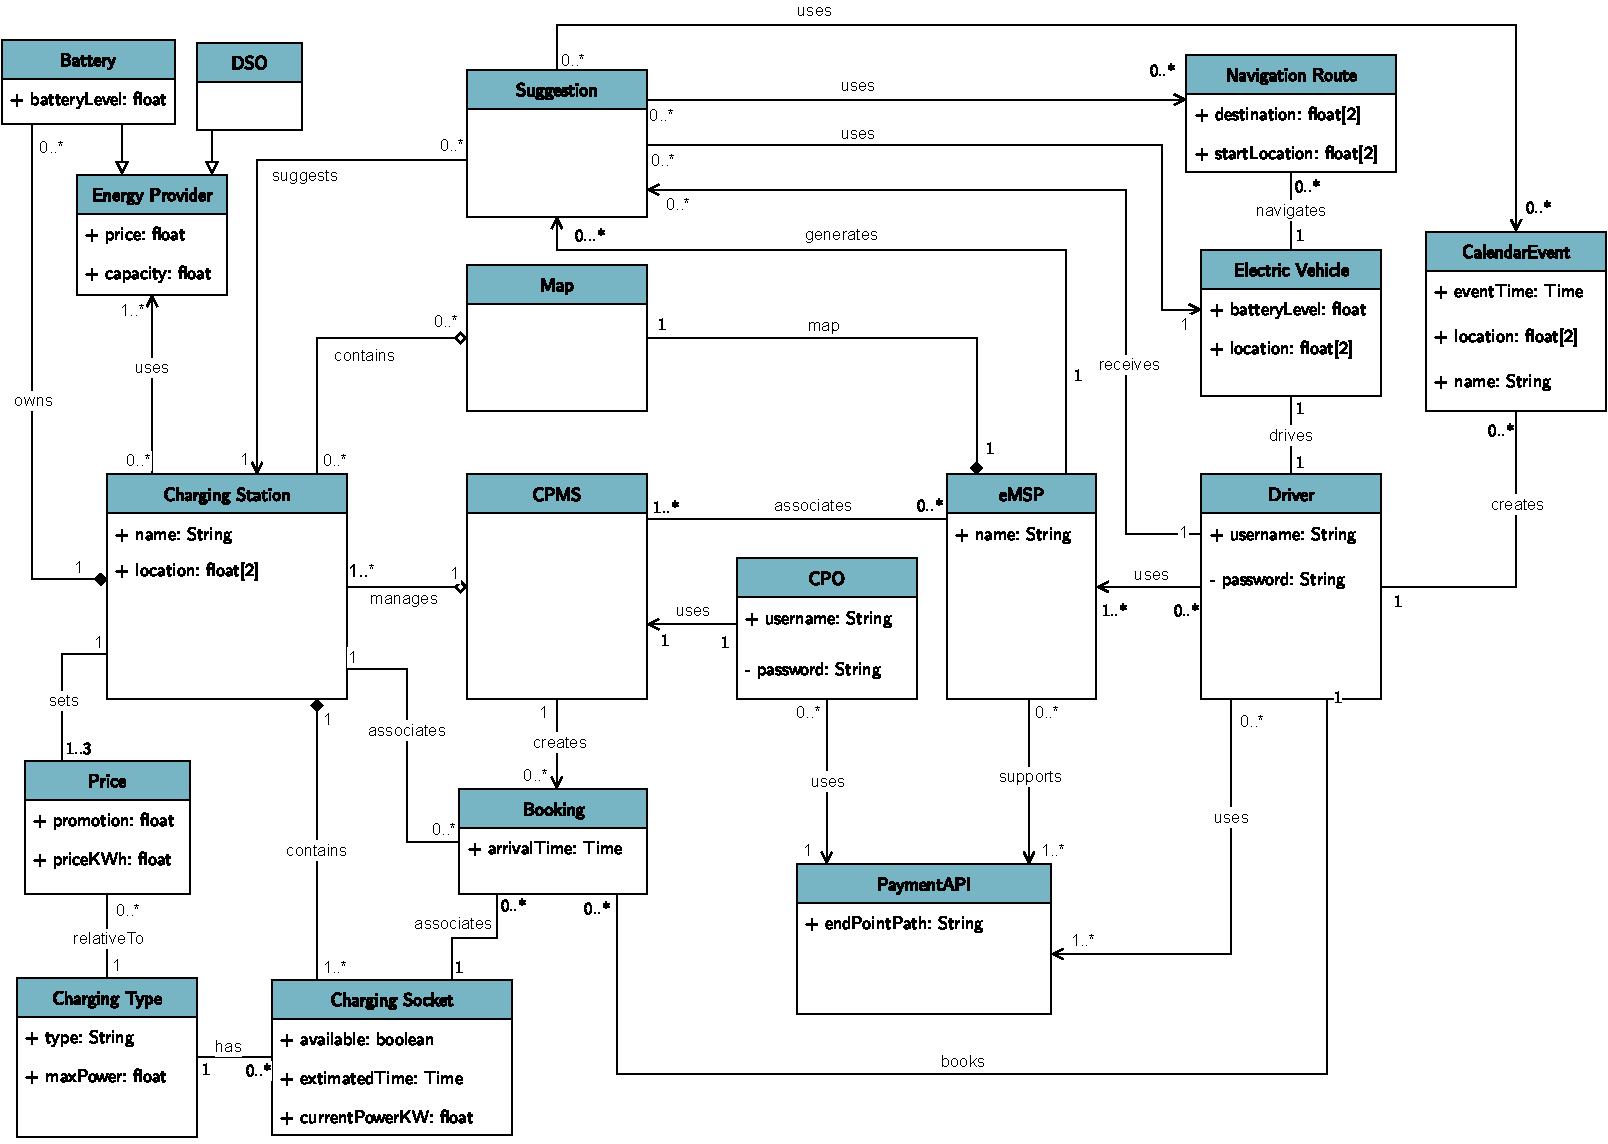
\includegraphics[
            width=\textwidth,
            height=\textheight,
            keepaspectratio]{classDiagram2}
        \caption{Class Diagram}
        \label{fig:classDiagram}
        \end{center}
    \end{figure}
    In this class diagram:
    \begin{itemize}
        \item Locations are represented with an array of 2 floats representing latitudes and longitudes.
        \item The Time type is used to represent a timestamp.
        \item The endPointPath attribute of the PaymentAPI class represents the URL from where the API sends requests.
    \end{itemize}     
    \newpage
\subsection{Dynamic Class Behaviour Models}
\label{subsec:statecharts}
The state diagrams listed below show the behaviour of the eMSP and the CPMS applications in their entirety.
\begin{itemize}
    \item \textbf{eMSP}
        \begin{figure}[H]
            \begin{center}
            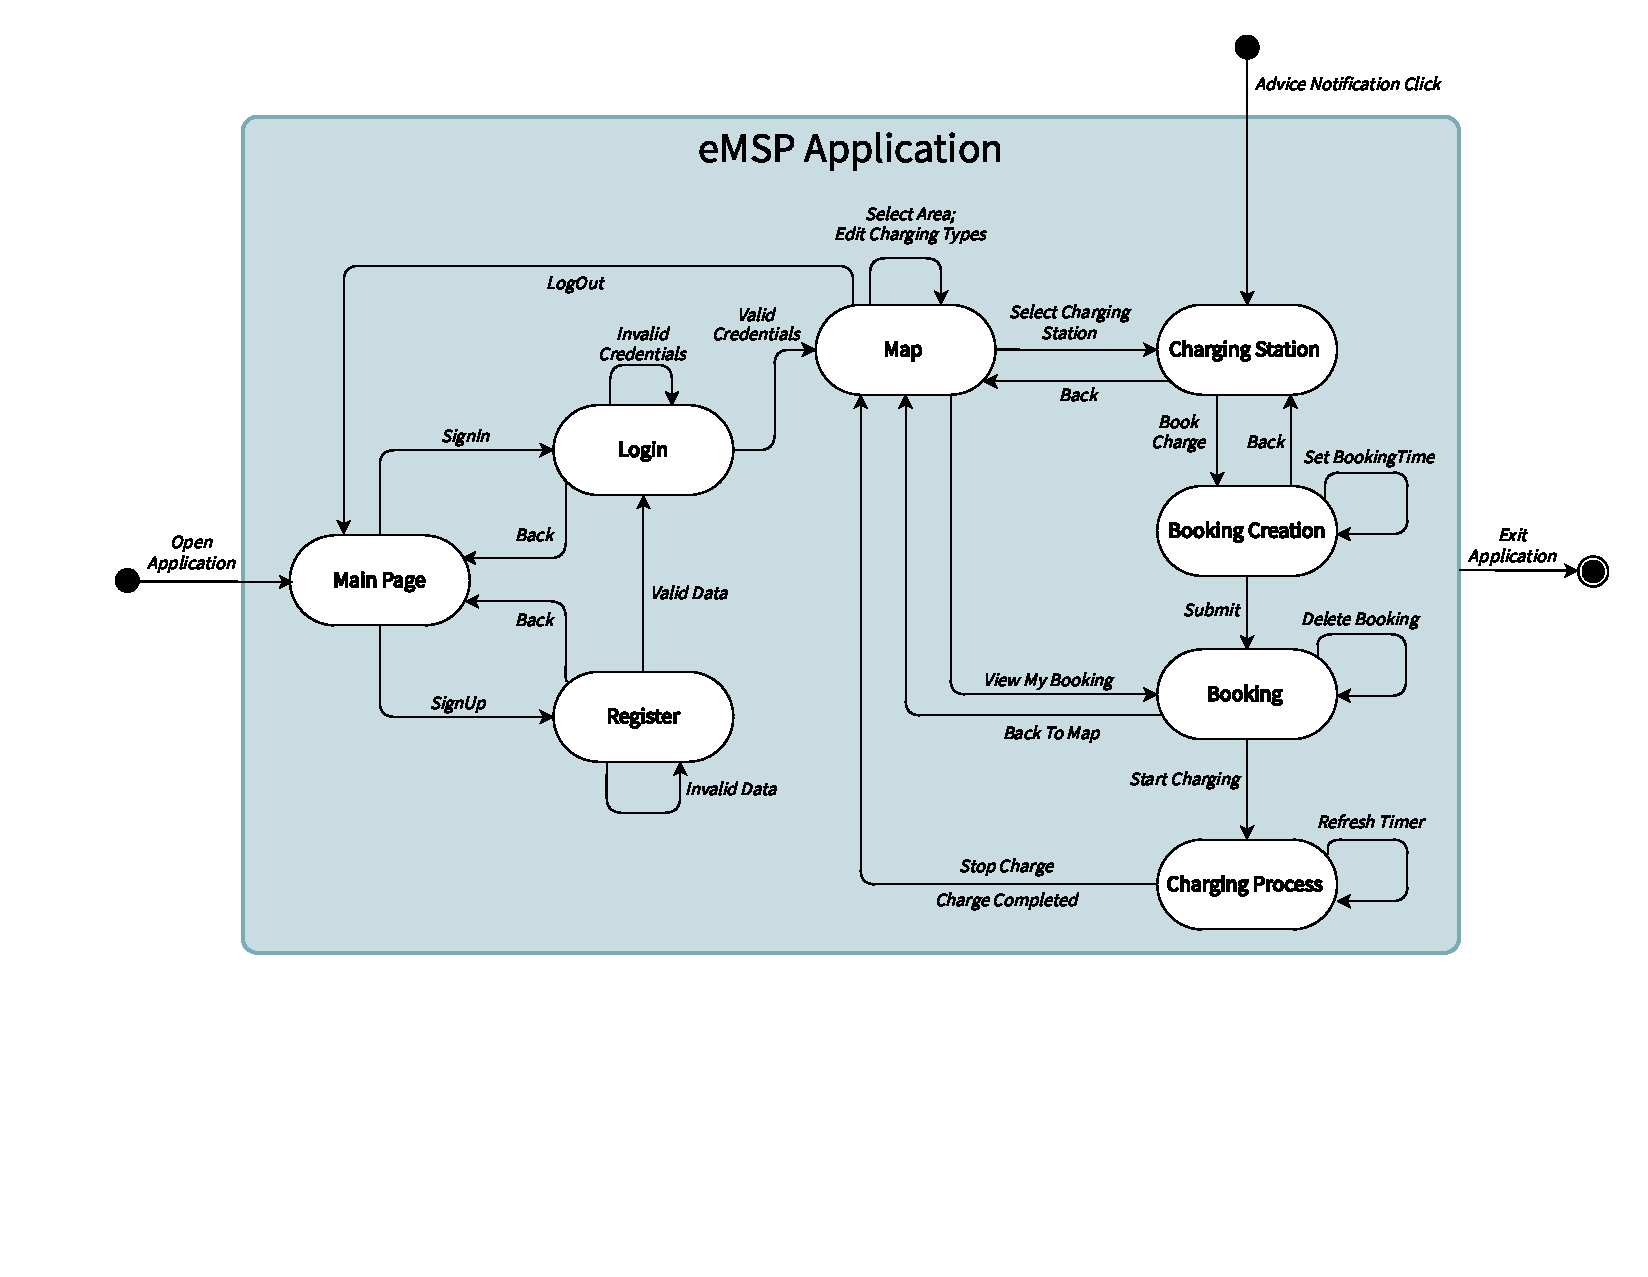
\includegraphics[
                width=\textwidth,
                height=\textheight,
                keepaspectratio]{StateCharts/eMSP}
            \caption{eMSP state diagram}
            \label{fig:eMSP}
            \end{center}
        \end{figure}
        \newpage
    \item \textbf{CPMS}
        \begin{figure}[H]
            \begin{center}
            \includegraphics[
                width=\textwidth,
                height=\textheight,
                keepaspectratio]{StateCharts/CPMS}
            \caption{CPMS state diagram}
            \label{fig:CPMS}
            \end{center}
        \end{figure}
\end{itemize}
\section{Product Functions} %AP
\label{sec:productFunctions}
In this section, the main functionalities of our system are presented and described in more detail. \\
\textbf{Functionalities offered to the drivers through the eMSP:}
\begin{itemize}
    \item \textbf{Check charging stations in the surrounding area:} 
    The driver can check nearby charging stations through a map of available ones. They have the possibility to select a specific station, in order to get more details about it, such as its availability, the charging price and any active offers.
    \item \textbf{Book a charge:} The driver can book a charge at a specific station up to a maximum amount of time in advance, through the details page of said station. They can select the type of charging socket, if available, that they want to use to charge the vehicle.
    \item \textbf{Start the charging process:} The driver, once they have driven to the charging station they booked in advance, can initiate the charging process through the application. If the vehicle is not well connected to the socket, the application will send a notification to the driver.
    \item \textbf{Proactive charge suggestion:} The driver can receive a suggestion to charge their vehicle based on their schedule and route to their destination. The system will evaluate the charging stations near the driver's route and if the prices are advantageous and the charging can fit into their schedule it will send a suggestion to the driver through the application.
\end{itemize}
\textbf{Functionalities offered to the CPOs through the CPMSs:}
\begin{itemize}
    \item \textbf{Charging Stations Management:} The CPO is able to manage all his charging stations: he can decide with which eMSPs to associate his CPMS and which charging stations will be managed by it.\\
    For those charging stations, the system will automatically handle the energy acquisition following the criteria set by the CPO, for example, based on the energy providers' prices, and their maximum power delivery capacity.\\
    For all the charging stations connected to the CPMS, the CPO will be able to set special offers for the charging prices and to visualize info about their internal status, such as the amount of energy available for the batteries, if available, the number of vehicles being charged and, for each charging vehicle, they can see the amount of power absorbed. 
    %\item \textbf{Check status of charging station:} The CPO can check through the application all the details about the managed charging stations, such as the amount of energy available for the batteries, if available, the number of vehicles being charged and, for each charging vehicle, they can see the amount of power absorbed.
    %\item \textbf{Decide where to buy energy:} The CPO can check a list of all available DSOs and decide which one to buy the energy from. This functionality can also be fully automated by the CPMS, if desired.
    %\item \textbf{Set a promotion for the charging price:} The CPO has the possibility to create an offer for any number of charging stations managed and, for each charging type, possibly set a different discount to the relative price. In this way, they can strategically reduce any price in order to attract more customers. 
    %\item \textbf{Select energy acquisition criteria:} The CPO has the possibility to decide which criteria the system has to follow while deciding which energy provider to acquire energy from. These criteria comprise the cost of the provider and/or its maximum capacity.
    %\item \textbf{Add a new charging station:} The CPO has the possibility to add a new charging station to the ones managed by his CPMS.
    %\item \textbf{eMSP association:} The CPO has the possibility to associate his CPMS to any existing eMSP in order to keep it updated about all his managed charging stations.
    %\item \textbf{Energy storage management:} The CPO can decide to store any additional energy bought from a DSO to the charging station's batteries, if available. Moreover, they can decide whether to utilize the batteries or the DSO as the source of energy to power the charging sockets. This functionality can also be fully automated by the CPMS, if desired.
\end{itemize}

\section{User Characteristics} %AS
The system can be exploited by the following actors:
\label{sec:userCharacteristics}
\begin{enumerate}
\item \textbf{Unregistered Driver}\\
A driver who needs to register to the eMSP platform before being able to use any of its functionalities.
\item \textbf{Driver}\\
A driver that is registered on the eMSP platform and can use all its functionalities.
\item \textbf{CPO}\\
A CPO registered on eMall who can use all the functionalities offered by its CMPS.
\end{enumerate}

\newpage
\section{Assumptions, Dependencies and Constraints}
\label{sec:assumptionsDependenciesConstraints}

\subsection{Domain Assumptions} %AS
\label{subsec:domainAssumptions}
    \begin{longtable}{| p{0.15\linewidth} | p{0.8\linewidth} |}
    \hline
    \rowcolor{bluepoli!40}
     \textbf{ID} & \textbf{Description} \T\B \\
    \hline \hline
    \textbf{D\row} & The Driver's vehicle is electric and has a battery able to be recharged with all the charging socket.\T\B\\
    \hline
    \textbf{D\row} & The Driver needs to know his personal data before signing up.\T\B\\
    \hline
    \textbf{D\row} & Every time the driver books a charging process then he will show up in time at the charging station.\T\B\\
    \hline
    \textbf{D\row} & When the Driver shows up during the time slot he booked, he’ll always find his booked charging socket available.\T\B\\
    \hline
    \textbf{D\row} & Every time the recharging process ends the driver leaves the station with his vehicle, which he first disconnects from the socket.\T\B\\
    \hline    
    \textbf{D\row} & If a vehicle is connected to a charging socket, then it delivers energy only after a driver starts the charging process booked for that socket.\T\B\\
    \hline
    \textbf{D\row} & The energy deployed by the charging socket is only used to recharge the vehicle battery.\T\B\\
    \hline
    \textbf{D\row} & Each charging socket has a unique ID relative to its charging station.\T\B\\
    \hline
    \textbf{D\row} & The driver is able to create a connection between his device and his vehicle that permits to retrieve from it reliable data about the navigation system, the vehicle’s battery status and location.\T\B\\
    \hline
    \textbf{D\row} & There exists a standard communication protocol that permits the charging sockets and charging stations to communicate with the CPMS in order to notify it of events like vehicle connection and disconnection or data about the charging status (completed, in process, remaining charging time). \T\B\\
    \hline    
    \textbf{D\row} & There exists a uniform API that allows retrieval information about DSOs, such as price and energy capacity. \T\B\\
    \hline
    \textbf{D\row} & There exists an external API that handles payments.\T\B\\
    \hline
    \textbf{D\row} & There exists an API endpoint where the eMSP can retrieve the map of a certain area.\T\B\\
    \hline
    \textbf{D\row} & There exists an API endpoint on eMall where the CPMS can retrieve a list of all eMSPs.\T\B\\
    \hline
    \textbf{D\row} & There exists an API endpoint on eMall where the CPMS can confirm the credentials inserted by the CPO \T\B \\
    \hline
    \caption{Domain Assumptions}
    \setcounter{row}{0}
\end{longtable}
\newcounter{case}
\newcommand\case{\stepcounter{case}\arabic{case}}
\chapter{SPECIFIC REQUIREMENTS}
\label{ch:specificRequirements}%
% The \label{...}% enables to remove the small indentation that is generated, always leave the % symbol.
\section{External Interface Requirements}
\label{sec:externalInterfaceRequirements}
\subsection{User Interfaces}
\label{subsec:userInterfaces}
The following mockups are presented here just to show an idea of the application
that will be in use by the Drivers and the one available to the CPOs. In Figure \ref{fig:map} and \ref{fig:book} are shown some of the functionalities available through the eMSP, such as the map and the charging station info. On the other hand, by figure \ref{fig:CPMS} it's possible to see the list of the CPO's managed charging stations, as well as the eMSP association functionality. The complete list of mockups (mobile app for eMSP and application for CMPS) will be available in the design document.
\begin{figure}[H]
    \begin{minipage}[t]{.35\textwidth} % not "0.5\textwidth"
    \includegraphics[width=\textwidth]{Mock/Map}
    \caption{Map}
    \label{fig:map}
\end{minipage}
\hfill
\begin{minipage}[t]{.35\textwidth}
    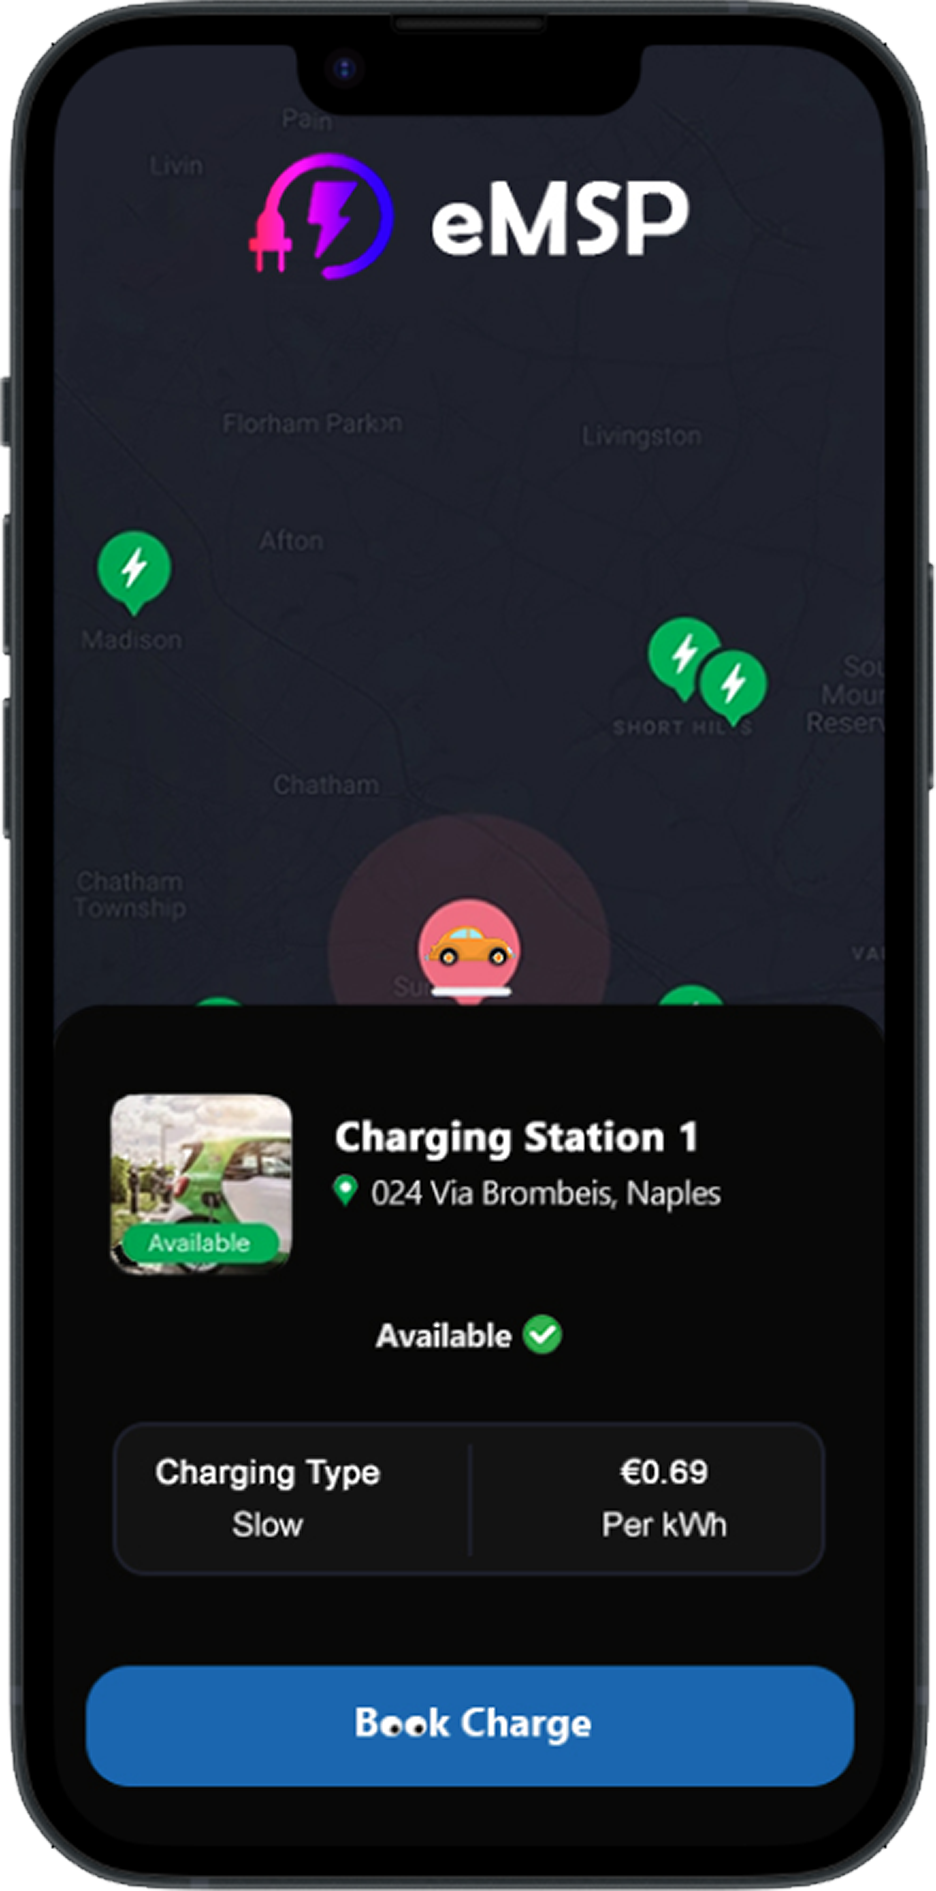
\includegraphics[width=\textwidth]{Mock/StationInfo}
    \caption{Station Info}
    \label{fig:book}
\end{minipage}
\end{figure}
\begin{figure}[H]
            \begin{center}
            \includegraphics[
                width=\textwidth,
                height=\textheight,
                keepaspectratio]{Mock/CPMS}
            \caption{CPMS Mockup}
            \label{fig:CPMS}
            \end{center}
        \end{figure}
\subsection{Hardware Interfaces}
\label{subsec:hardwareInterfaces}
\begin{itemize}
    \item \textbf{Vehicle Interface}: Since the system requires to access info from the Driver's vehicle, such as the battery level, the location or the navigation route, it is necessary to establish a connection between the two of them. This should be done by the Driver through his device in order to let him receive suggestions.
    \item \textbf{Charging Station Interface}: In order to add and manage charging stations to the system there must be an interface between the two of them that permits the exchange of data through a standard protocol.
    \item \textbf{Charging Socket Interface}: In order to manage the charging process, check both its status and the connection between the vehicle and its connected socket, there must be an interface between the system and charging sockets that permits the exchange of data through a standard protocol.
    %\item \textbf{eMSP}: \\
     %   In order to install and utilize the system the Driver needs to have a mobile device with an internet connection. It should be able to run the application, which requires rendering of maps. Furthermore, it should be able to connect with his vehicle. The connection between the mobile device and the vehicle should allow to extrapolate data, such as battery status and navigation routes, from the vehicle and send it to eMSP through the mobile device. 
    %\item \textbf{CPMS}: \\
     %   In order to install and utilize the system, the CPO should have access to a machine capable of hosting the CPMS Server and another device, such as any computer, capable of elaborating and making requests to the CPMS server. The server machine is required to have a stable internet connection in order be able to talk with eMSPs subsystems and receive multiple requests from them.
\end{itemize}
\subsection{Software Interfaces}
\label{subsec:softwareInterfaces}
The CPMS and eMSP communicate with each other through a uniform API, in order to exchange information. In particular, the CPMS has to update all the eMSPs that are associated with him about socket availability and stations' charging prices; meanwhile, the eMSP has to communicate with the CPMS in order to let the Driver perform operations for recharging his vehicle and create/delete bookings. In order to do so, all the CPMSs and the eMSPs should have the same external interface protocol and attain themselves to this standard.
\subsection{Communication Interfaces}
\label{subsec:communicationInterfaces}
The systems, both the eMSP and the CPMS, communicate with external APIs in order to provide all the different functions described in section \ref{sec:productFunctions}.
\begin{itemize}
    %\item \textbf{Charging station} - The CPMS communicates with charging stations and charging socket in order to receive data about physical events such as vehicle connected or charge finished and perform operations, like starting a charge. 
    \item \textbf{Payment API} - In order for the Driver to pay the relative CPO for the given charging service, the eMSP uses an external API that allows and manages payments.
    \item \textbf{Maps API} - In order to show the Driver where all the charging stations are located, the eMSP uses an external API that provides up-to-date maps.
    \item \textbf{Calendar API} - In order to generate suggestions for the Driver, the eMSP application can check the calendar events through this API.
    \item \textbf{eMall API} - The eMall system provides the following APIs in order to let the eMSP and the CPMS communicate with it:
        \begin{itemize}
            \item \textbf{Confirming credentials} - The CPO credentials used to access the CPMS are authenticated on the eMall system.
            \item \textbf{eMSP List} - The CPMS retrieves a list of all the existing eMSPs from the eMall system, in order to show them to the CPO.
        \end{itemize}
   \item \textbf{DSO API} - The CPMS uses an external uniform API to retrieve the DSOs prices and energy capacity, in order to choose which one to get energy from. 
   %\item \textbf{Charging Station modules} - The CPMS needs to be able to communicate with the charging station in order to detect whether a new one has been managed by the CPO.     
\end{itemize}
\label{subsec:sequenceDiagrams}
\section{Functional Requirements}
\label{sec:functionalRequirements}
\subsection{Use Case Diagrams}
\begin{enumerate}
    \item \textbf{Unregistered Driver}
        \begin{figure}[H]
            \begin{center}
            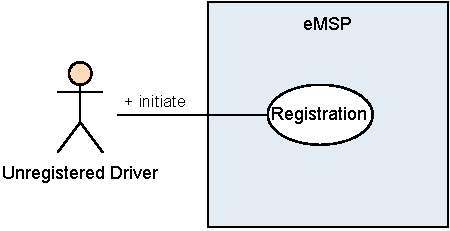
\includegraphics[
                width=0.6\textwidth,
                height=\textheight,
                keepaspectratio]{UseCaseDia/UnregisteredDriver}
            \caption{Use case diagram for an Unregistered Driver}
            \label{fig:UnregisteredDriver}
            \end{center}
        \end{figure}
        \newpage
    \item \textbf{Driver}
        \begin{figure}[H]
            \begin{center}
            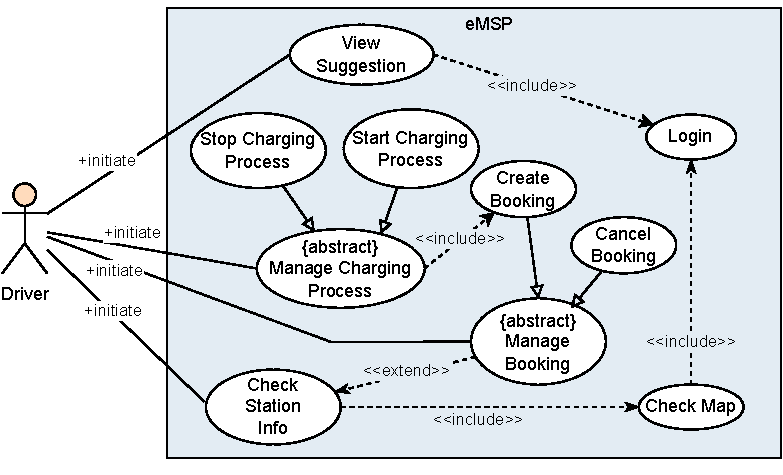
\includegraphics[
                width=\textwidth,
                height=\textheight,
                keepaspectratio]{UseCaseDia/Driver}
            \caption{Use case diagram for a Driver}
            \label{fig:UnregisteredDriver}
            \end{center}
        \end{figure}
    \item \textbf{CPO}
        \begin{figure}[H]
            \begin{center}
            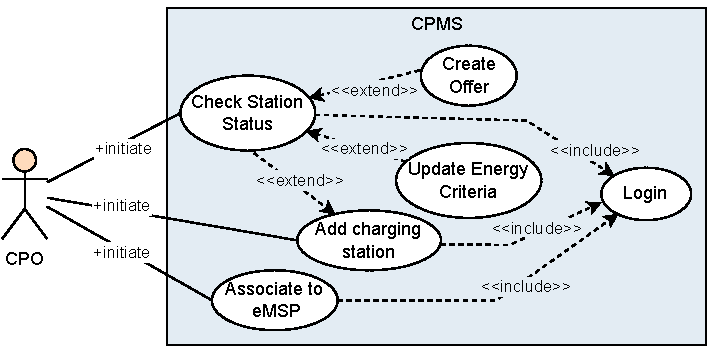
\includegraphics[
                width=\textwidth,
                height=\textheight,
                keepaspectratio]{UseCaseDia/CPO}
            \caption{Use case diagram for a CPO}
            \label{fig:UnregisteredDriver}
            \end{center}
        \end{figure}
\end{enumerate}
\label{subsec:useCaseDiagrams}
\newpage
\subsection{Use Cases}
\label{subsec:useCases}
\textbf{Note}: In the following use cases we assume no internet connection failures.
% belliximo template per gli use cases by Andrea BIBA
% se si usa longtable gli elenchi escono con un padding orribile
% quindi meglio tenere tabular
\begin{enumerate}
    \item \textbf{Driver Registration} 
    \begin{table}[H]
        \centering
    \begin{tabular}{| >{\columncolor{bluepoli!15}}p{0.30\linewidth} |p{0.7\linewidth} |}
        \hline
        \rowcolor{bluepoli!40}
        \textbf{Use Case \case} & \textbf{Driver Registration} \T\B \\
        \hline 
        \hline
        \textbf{Actor(s)} & Unregistered Driver \T\B\\
        \hline
        \textbf{Entry Condition} & The driver does not have an account and is on the initial view of the eMSP \T\B\\ 
        \hline
        \textbf{Event Flow} &     
        \begin{enumerate}
            \item The Unregistered Driver press the "Register" button
            \item The Unregistered Driver enters the username, password, birth date, email address and a payment method
            \item The Unregistered Driver submits the compiled form
            \item The eMSP processes the request and shows a success message
        \end{enumerate}\T\B\\
        \hline
        \textbf{Exit Condition} & An account is created \T\B\\
        \hline
        \textbf{Exception} & The driver does not enter all mandatory data. The exception is notified to the Driver. \T\B\\
        \hline
    \end{tabular}
    \end{table}
    \item \textbf{ Driver Login} 
    \begin{table}[H]
        \centering
    \begin{tabular}{| >{\columncolor{bluepoli!15}}p{0.30\linewidth} |p{0.7\linewidth} |}
        \hline
        \rowcolor{bluepoli!40}
        \textbf{Use Case \case} & \textbf{Driver Login} \T\B \\
        \hline 
        \hline
        \textbf{Actor(s)} & Driver \T\B\\
        \hline
        \textbf{Entry Condition} & Driver not logged in and on the eMSP main page \T\B\\ 
        \hline
        \textbf{Event Flow} &     
        \begin{enumerate}
            \item The Driver press the "Login" button
            \item The Driver submits his credentials such as username and password 
            \item The eMSP validates his credentials and shows a success message
        \end{enumerate}\T\B\\
        \hline
        \textbf{Exit Condition} & The Driver is logged into the eMSP\T\B\\
        \hline
        \textbf{Exception} & 
         The Driver enters invalid credentials. The exception is notified to the Driver. \T\B\\
        \hline
    \end{tabular}
    \end{table}
    \newpage
    \item \textbf{ Driver checks map}
    \begin{table}[H]
        \centering
    \begin{tabular}{| >{\columncolor{bluepoli!15}}p{0.30\linewidth} |p{0.7\linewidth} |}
        \hline
        \rowcolor{bluepoli!40}
        \textbf{Use Case \case} & \textbf{Driver checks map} \T\B \\
        \hline 
        \hline
        \textbf{Actor(s)} & Driver \T\B\\
        \hline
        \textbf{Entry Condition} & Driver is logged in \T\B\\ 
        \hline
        \textbf{Event Flow} &     
        \begin{enumerate}
            \item The Driver opens the eMSP application and gets on the Map view
            \item (opt) The Driver moves to the area in which he wants to see all the charging stations
            \item (opt) The Driver selects the charging type filter to apply to the map
            \item The eMSP processes the request and returns the charging stations on the map that match the filters in that area
        \end{enumerate}\T\B\\
        \hline
        \textbf{Exit Condition} & All the stations are shown to the Driver\T\B\\
        \hline
        \textbf{Exception} & There are no available stations matching the filter in the requested area. The system sends a notification to warn the Driver. \T\B\\
        \hline
    \end{tabular}
    \end{table}
    \item \textbf{ Driver checks charging station info}
    \begin{table}[H]
        \centering
    \begin{tabular}{| >{\columncolor{bluepoli!15}}p{0.30\linewidth} |p{0.7\linewidth} |}
        \hline
        \rowcolor{bluepoli!40}
        \textbf{Use Case \case} & \textbf{Driver checks charging station info} \T\B \\
        \hline 
        \hline
        \textbf{Actor(s)} & Driver \T\B\\
        \hline
        \textbf{Entry Condition} & Driver is on the map page \T\B\\ 
        \hline
        \textbf{Event Flow} &     
        \begin{enumerate}
            \item The Driver clicks on one of the shown charging stations
            \item The eMSP processes the request and returns the info of that charging station, such as its charging prices for each charging type, the address and the availability
            \item The Driver sees the received info
        \end{enumerate}\T\B\\
        \hline
        \textbf{Exit Condition} & Info of the selected station is correctly shown to the Driver. \T\B\\
        \hline
        \textbf{Exception} & None \T\B\\
        \hline
    \end{tabular}
    \end{table}
    \newpage
    \item \textbf{Book a charge}
    \begin{table}[H]
        \centering
    \begin{tabular}{| >{\columncolor{bluepoli!15}}p{0.30\linewidth} |p{0.7\linewidth} |}
        \hline
        \rowcolor{bluepoli!40}
        \textbf{Use Case \case} & \textbf{Book a charge} \T\B \\
        \hline 
        \hline
        \textbf{Actor(s)} & Driver \T\B\\
        \hline
        \textbf{Entry Condition} & Driver is checking the details of a station \T\B\\ 
        \hline
        \textbf{Event Flow} &     
        \begin{enumerate}
            \item The Driver clicks on the "Book Charge" button
            \item The Driver selects the arrival time
            \item The Driver clicks on "Submit" and sends the request
            \item The eMSP notifies the user that he has successfully booked a charge and the ID of the charging socket
        \end{enumerate}\T\B\\
        \hline
        \textbf{Exit Condition} & The charge has been correctly booked \T\B\\
        \hline
        \textbf{Exception} & An exception is thrown to the eMSP by the CMPS. The exception message is notified to the Driver.\T\B\\
        \hline
    \end{tabular}
    \end{table}
    \item \textbf{Cancel a booked charge}
    \begin{table}[H]
        \centering
    \begin{tabular}{| >{\columncolor{bluepoli!15}}p{0.30\linewidth} |p{0.7\linewidth} |}
        \hline
        \rowcolor{bluepoli!40}
        \textbf{Use Case \case} & \textbf{Cancel a booked charge} \T\B \\
        \hline 
        \hline
        \textbf{Actor(s)} & Driver \T\B\\
        \hline
        \textbf{Entry Condition} & Driver has booked a charge\T\B\\ 
        \hline
        \textbf{Event Flow} &     
        \begin{enumerate}
            \item The Driver clicks on the Booked Charge button
            \item The Driver clicks on the "Delete Booking" button
            \item The eMSP notifies the user that the booked charge has been deleted
        \end{enumerate}\T\B\\
        \hline
        \textbf{Exit Condition} & The booked charge has been deleted \T\B\\
        \hline
        \textbf{Exception} & An exception is thrown to the eMSP by the CMPS. The exception message is notified to the Driver. \T\B\\
        \hline
    \end{tabular}
    \end{table}
    \newpage
    \item \textbf{Start charging process}
    \begin{table}[H]
        \centering
    \begin{tabular}{| >{\columncolor{bluepoli!15}}p{0.30\linewidth} |p{0.7\linewidth} |}
        \hline
        \rowcolor{bluepoli!40}
        \textbf{Use Case \case} & \textbf{Start charging process} \T\B \\
        \hline 
        \hline
        \textbf{Actor(s)} & Driver \T\B\\
        \hline
        \textbf{Entry Condition} & The driver has booked a charge and is arrived at the charging station \T\B\\ 
        \hline
        \textbf{Event Flow} &     
        \begin{enumerate}     
            \item The Driver clicks on the Booked Charge button and checks the socket ID he has booked   
            \item The Driver plugs his vehicle to the socket with the ID booked
            \item The Driver clicks on the "Start Charge" button
            \item The eMSP processes the request and notifies the user that the charging process has been started
            \item The Driver sees the estimated time for the charge to end
        \end{enumerate}\T\B\\
        \hline
        \textbf{Exit Condition} & The charge is started \T\B\\
        \hline
        \textbf{Exceptions} & 
            The charge can't be started because the vehicle is not well connected with the socket. The exception is notified to the Driver. 
        \\
        \hline
    \end{tabular}
    \end{table}
    \item \textbf{Stop charging process}
    \begin{table}[H]
        \centering
    \begin{tabular}{| >{\columncolor{bluepoli!15}}p{0.30\linewidth} |p{0.7\linewidth} |}
        \hline
        \rowcolor{bluepoli!40}
        \textbf{Use Case \case} & \textbf{Stop charging process} \T\B \\
        \hline 
        \hline
        \textbf{Actor(s)} & Driver \T\B\\
        \hline
        \textbf{Entry Condition} & The driver is checking the detail of his charging process \T\B\\ 
        \hline
        \textbf{Event Flow} &     
        \begin{enumerate}
            \item The Driver clicks on the "Stop Charge" button
            \item The eMSP processes the request and notifies the user that the charging process has been stopped
            \item The eMSP notifies the user that the payment was successful
        \end{enumerate}\T\B\\
        \hline
        \textbf{Exit Condition} & The charge has been ended \T\B\\
        \hline
        \textbf{Exception} & The eMSP can't process the booking request due to an error while communicating with the CMPS. The exception is notified to the Driver. \T\B\\
        \hline
    \end{tabular}
    \end{table}
    \newpage
    \item \textbf{Suggestion Notification}
    \begin{table}[H]
        \centering
    \begin{tabular}{| >{\columncolor{bluepoli!15}}p{0.30\linewidth} |p{0.7\linewidth} |}
        \hline
        \rowcolor{bluepoli!40}
        \textbf{Use Case \case} & \textbf{Suggestion Notification} \T\B \\
        \hline 
        \hline
        \textbf{Actor(s)} & Driver \T\B\\
        \hline
        \textbf{Entry Condition} & The Driver has authorized the systems to read his data (calendar, vehicle's navigation routes, vehicle's location and vehicle's battery status) and receives a notification containing a suggested charging station where to charge his vehicle.  \T\B\\ 
        \hline
        \textbf{Event Flow} &
        (opt - Driver can ignore the notification)
        \begin{enumerate}
            \item The Driver clicks on the notification.
            \item The Driver is redirected to the station's info page.
        \end{enumerate}\T\B\\
        \hline
        \textbf{Exit Conditions} & 
        \begin{itemize}
            \item The Driver is on the station info page.
            \item The Driver ignores the notification.
        \end{itemize}  \T\B\\
        \hline
        \textbf{Exception} & None \T\B\\
        \hline
    \end{tabular}
    \end{table}
\item \textbf{CPO Login}
    \begin{table}[H]
        \centering
    \begin{tabular}{| >{\columncolor{bluepoli!15}}p{0.30\linewidth} |p{0.7\linewidth} |}
        \hline
        \rowcolor{bluepoli!40}
        \textbf{Use Case \case} & \textbf{CPO Login} \T\B \\
        \hline 
        \hline
        \textbf{Actor(s)} & CPO \T\B\\
        \hline
        \textbf{Entry Condition} & The CPO is not logged in and is on the initial view of the CPMS \T\B\\ 
        \hline
        \textbf{Event Flow} &     
        \begin{enumerate}
            \item The CPO presses the "Login" button.
            \item The CPO submits his credentials such as email and password.
            \item The CPMS validates his credentials and shows a success message.
        \end{enumerate}\T\B\\
        \hline
        \textbf{Exit Condition} & The CPO is logged into the CPMS and sees the list of his managed charging stations. \T\B\\
        \hline
        \textbf{Exception} & The CPO enters invalid credentials. The exception is notified to the CPO. \T\B\\
        \hline
        \end{tabular}
        \end{table}
        \newpage
\item \textbf{View managed charging station status}
    \begin{table}[H]
        \centering
    \begin{tabular}{| >{\columncolor{bluepoli!15}}p{0.30\linewidth} |p{0.7\linewidth} |}
        \hline
        \rowcolor{bluepoli!40}
        \textbf{Use Case \case} & \textbf{View managed charging station status} \T\B \\
        \hline 
        \hline
        \textbf{Actor(s)} & CPO \T\B\\
        \hline
        \textbf{Entry Condition} & The CPO is logged in \T\B\\ 
        \hline
        \textbf{Event Flow} &    
        \begin{enumerate}
            \item The CPO clicks on one of the "Select Station" buttons of one of the listed charging stations.
            \item The CPO visualizes info related to that station such as batteries energy (if available), the number of connected vehicles, their power absorption and their estimated remaining charging time.
        \end{enumerate}\T\B\\
        \hline
        \textbf{Exit Condition} & The station info is correctly visualized \T\B\\
        \hline
        \textbf{Exception} & None. \T\B\\
        \hline
        \end{tabular}
        \end{table}
    %\item \textbf{Checks info}
  %  \begin{table}[H]
     %   \centering
    %\begin{tabular}{| >{\columncolor{bluepoli!15}}p{0.30\linewidth} |p{0.7\linewidth} |}
    %    \hline
    %   \rowcolor{bluepoli!40}
     %   \textbf{Use Case \case} & \textbf{Check info} \T\B \\
     %   \hline 
     %   \hline
     %   \textbf{Actor(s)} & CPO \T\B\\
     %   \hline
      %  \textbf{Entry Condition} & The CPO is logged in and is on the View managed stations page\T\B\\ 
       % \hline
        %\textbf{Event Flow} &     
     %%   \begin{enumerate}
    %        \item The CPO selects the data that he wants to check such as batteries status, number of vehicle, power absorption. 
   %         \item The CPMS processes the information and show the details of the data.
   %     \end{enumerate}\T\B\\
  %      \hline
  %      \textbf{Exit Condition} & The data details are showed to the CPO \T\B\\
  %      \hline
  %      \textbf{Exception} & None \T\B\\
  %      \hline
  %      \end{tabular}
 %       \end{table}
 
\item \textbf{Set an Offer}
    \begin{table}[H]
        \centering
    \begin{tabular}{| >{\columncolor{bluepoli!15}}p{0.30\linewidth} |p{0.7\linewidth} |}
        \hline
        \rowcolor{bluepoli!40}
        \textbf{Use Case \case} & \textbf{Set an Offer} \T\B \\
        \hline 
        \hline
        \textbf{Actor(s)} & CPO \T\B\\
        \hline
        \textbf{Entry Condition} & The CPO is logged in and on a managed station page \T\B\\ 
        \hline
        \textbf{Event Flow} &     
        \begin{enumerate}
            \item The CPO clicks on the "Set New Offer" button.
            %\item The CPO selects one or more of the managed charging stations.
            %\item The CPO clicks on the "Next" button.
            \item The CPO selects the amount of discount for each of the charging types wanted.
            \item The CPO selects the expiration date for the offer.
            \item The CPO clicks the "Submit" button.
            \item The CPMS processes the information and shows a success message.
        \end{enumerate}\T\B\\
        \hline
        \textbf{Exit Condition} & The offer has been applied to the selected charging station \T\B\\
        \hline
        \textbf{Exception} & The CPO enters an invalid discount amount or an invalid expiration date. The exception is notified to the CPO. \T\B\\
        \hline
        \end{tabular}
        \end{table}
        \newpage
\item \textbf{Update energy criteria}
    \begin{table}[H]
        \centering
    \begin{tabular}{| >{\columncolor{bluepoli!15}}p{0.30\linewidth} |p{0.7\linewidth} |}
        \hline
        \rowcolor{bluepoli!40}
        \textbf{Use Case \case} & \textbf{Update energy criteria} \T\B \\
        \hline 
        \hline
        \textbf{Actor(s)} & CPO \T\B\\
        \hline
        \textbf{Entry Condition} & The CPO is logged in and on a managed station page \T\B\\ 
        \hline
        \textbf{Event Flow} &     
        \begin{enumerate}
            \item The CPO clicks on the "Energy criteria" button.
            \item (opt) The CPO modifies the energy sale percentage revenue.
            \item (opt) The CPO modifies the energy acquisition criteria.
            \item The CPO clicks the "Update" button.
            \item The CPMS processes the information and shows a success message.
        \end{enumerate}\T\B\\
        \hline
        \textbf{Exit Condition} & The energy criteria have been correctly updated for the selected charging station. \T\B\\
        \hline
        \textbf{Exception} & The new criteria are invalid. The exception is notified to the CPO. \T\B\\
        \hline
        \end{tabular}
        \end{table}  
\item \textbf{Associate eMSP}
    \begin{table}[H]
        \centering
    \begin{tabular}{| >{\columncolor{bluepoli!15}}p{0.30\linewidth} |p{0.7\linewidth} |}
        \hline
        \rowcolor{bluepoli!40}
        \textbf{Use Case \case} & \textbf{Associate eMSP} \T\B \\
        \hline 
        \hline
        \textbf{Actor(s)} & CPO \T\B\\
        \hline
        \textbf{Entry Condition} & The CPO is logged in \T\B\\ 
        \hline
        \textbf{Event Flow} &     
        \begin{enumerate}
            \item The CPO clicks on the "Associate eMSPs" button
            \item The CPMS shows a list of all the existing eMSPs that are not associated yet
            \item The CPO selects the eMSPs he wants to associate with 
            \item The CPO clicks on the "Submit Selection".
            \item The CPMS processes the request and sends a success message
        \end{enumerate}\T\B\\
        \hline
        \textbf{Exit Condition} & The selected eMSPs are now associated with the CPMS. \T\B\\
        \hline
        \textbf{Exception} & The CPMS can't connect with one of the selected eMSP. The exception is notified to the CPO. \T\B\\
        \hline
        \end{tabular}
        \end{table}  
        \newpage
\item \textbf{Add charging station}
    \begin{table}[H]
        \centering
    \begin{tabular}{| >{\columncolor{bluepoli!15}}p{0.30\linewidth} |p{0.7\linewidth} |}
        \hline
        \rowcolor{bluepoli!40}
        \textbf{Use Case \case} & \textbf{Add charging station} \T\B \\
        \hline 
        \hline
        \textbf{Actor(s)} & CPO \T\B\\
        \hline
        \textbf{Entry Condition} & The CPO is logged in and has a charging station not yet connected to the system. \T\B\\ 
        \hline
        \textbf{Event Flow} &     
        \begin{enumerate}
            \item The CPO clicks on the "Add charging station" button.
            \item The CPMS shows a list of detected charging stations.
            \item The CPO connects the new charging station to one of the available stations from the list.           
            \item The CPO inserts the new charging station data e.g. name, location and supported charging types.
            \item The CPO clicks the "Submit" button.
            \item The CPMS processes the request and shows a success message.
            \item The CPMS shows the energy criteria page of the new charging station.
        \end{enumerate}\T\B\\
        \hline
        \textbf{Exit Condition} & The charging station has been correctly added and the system is showing the energy criteria page of that station. \T\B\\
        \hline
        \textbf{Exception} & The new station data is invalid. The exception is notified to the CPO. \T\B\\
        \hline
        \end{tabular}
        \end{table}  
\end{enumerate}
%[a4paper, includehead, headheight=0.6cm, inner=2.5cm ,outer=2.5cm, top=1.5cm, bottom=2.5cm]{geometry}
\newgeometry{inner=2.5cm ,outer=2.5cm, top=1.4cm,bottom=1cm, includefoot}
\subsection{Sequence Diagrams}
\begin{tabbing}
    \textbf{Note}: \= In the following sequence diagrams we assume no internet connection failures. \\
    \> Synchronous responses are a result of actions performed locally in the application.
\end{tabbing}
\begin{enumerate}
        \item \textbf{Driver Registration}
        \begin{figure}[H]
            \begin{center}
            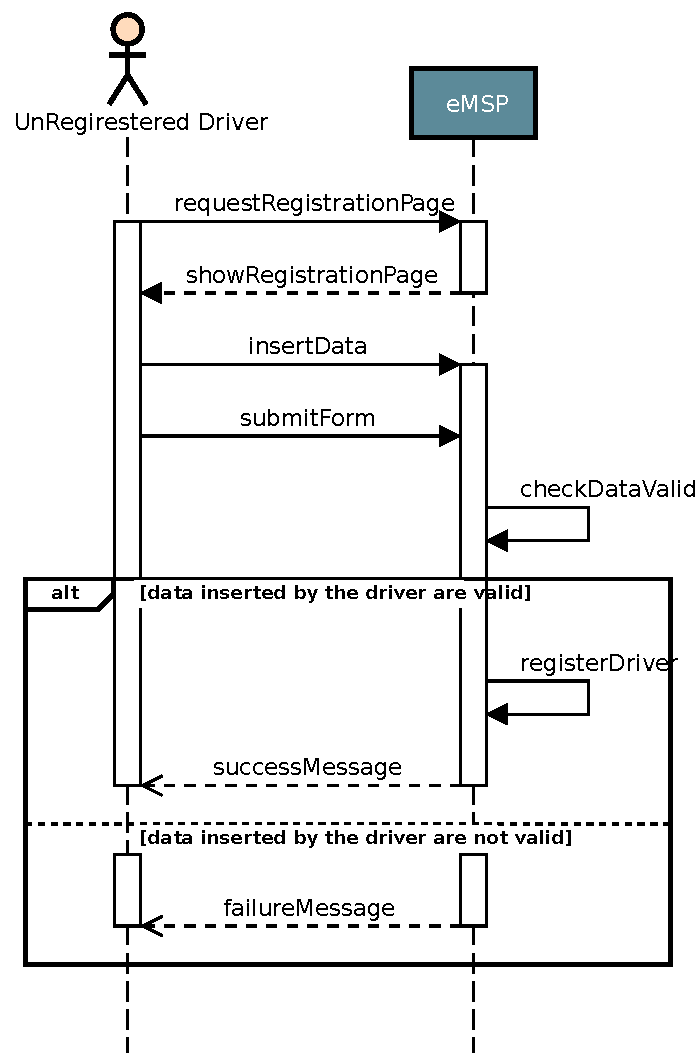
\includegraphics[
                width=\textwidth,
                height=0.35\textheight,
                keepaspectratio]{SeqDia/Register}
            \caption{Registration of a driver}
            \label{fig:Register}
            \end{center}
        \end{figure}
        \item \textbf{Driver Login}
        \begin{figure}[H]
            \begin{center}
            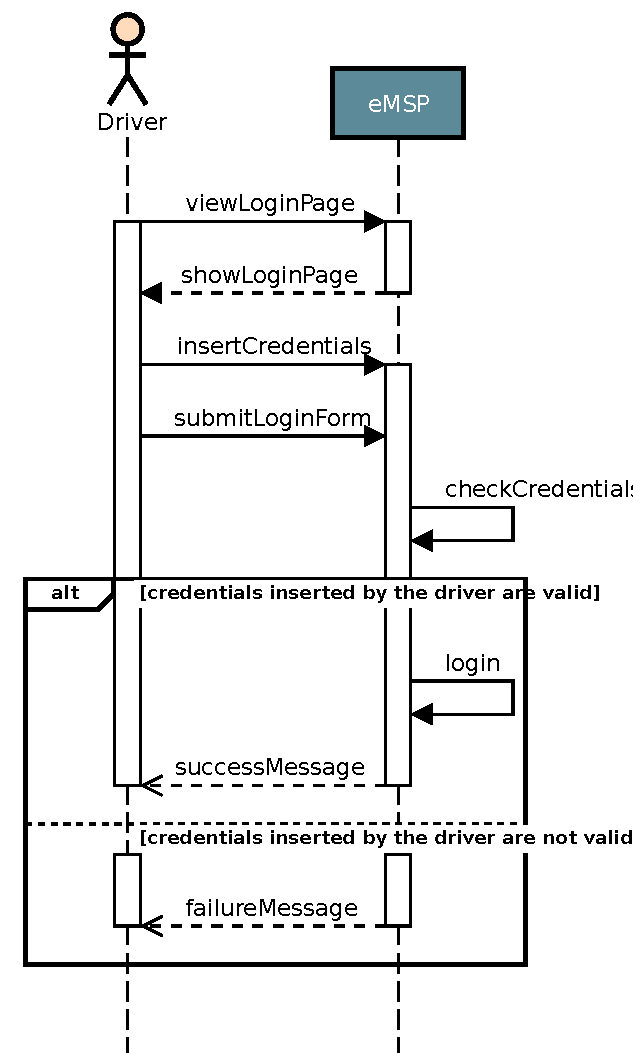
\includegraphics[
                width=\textwidth,
                height=0.35\textheight,
                keepaspectratio]{SeqDia/DriverLogin}
            \caption{Login of a Driver}
            \label{fig:DriverLogin}
            \end{center}
        \end{figure}
        \newpage
        \item \textbf{Check Map}
        \begin{figure}[H]
            \begin{center}
            \includegraphics[
                width=\textwidth,
                height=0.43\textheight,
                keepaspectratio]{SeqDia/Map}
            \caption{Check Map of the eMSP}
            \label{fig:Map}
            \end{center}
        \end{figure}
        \item \textbf{Check Station Info}
        \begin{figure}[H]
            \begin{center}
            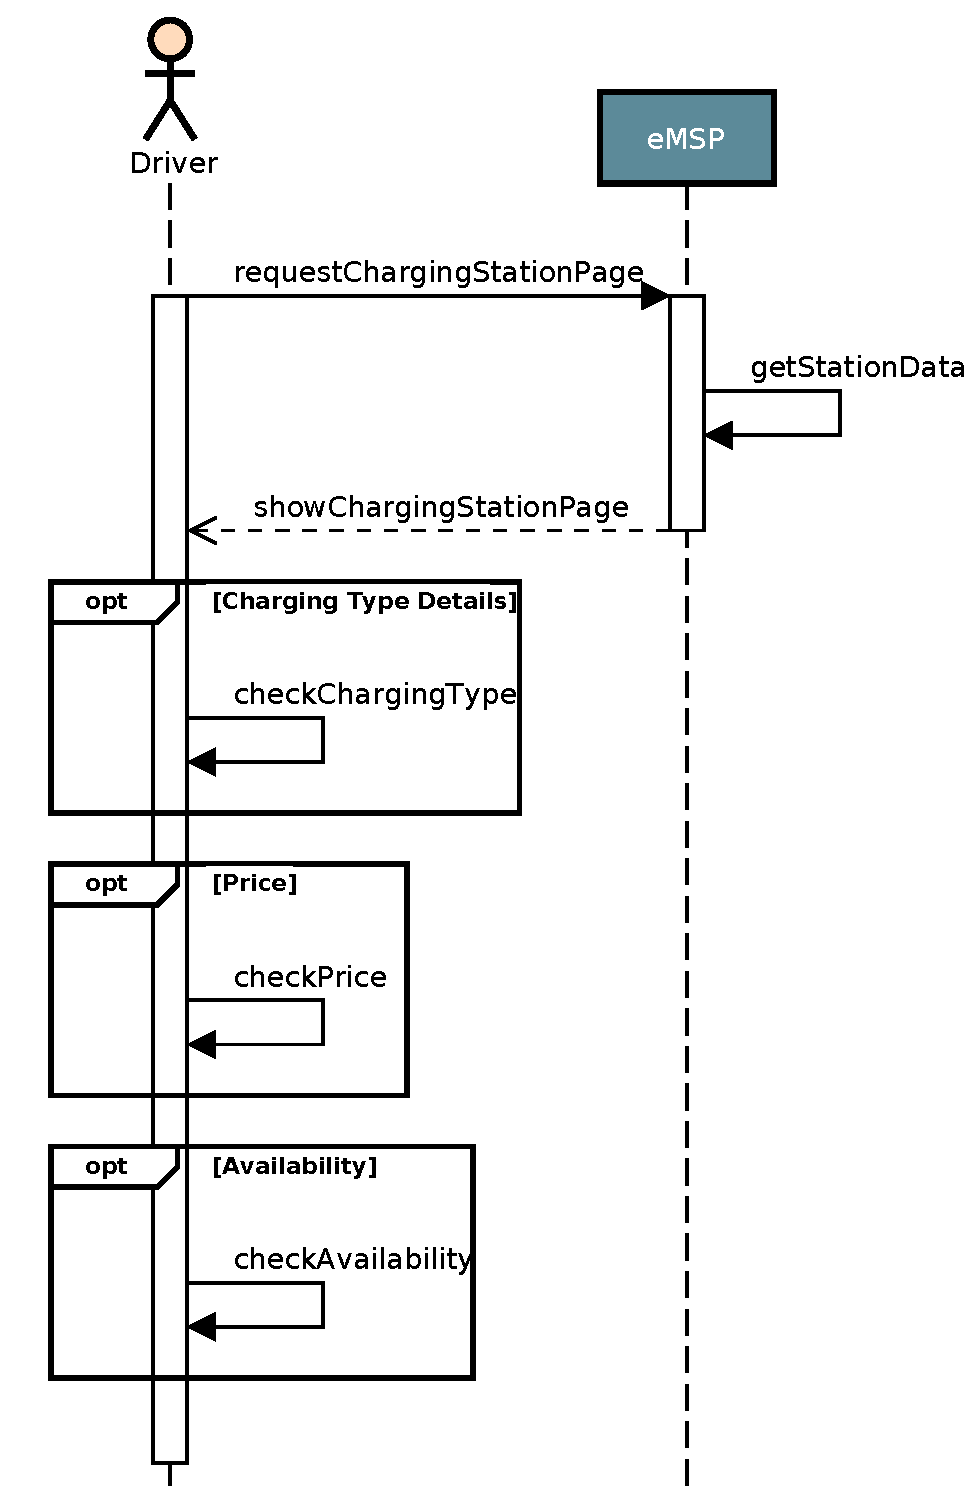
\includegraphics[
                width=\textwidth,
                height=0.4\textheight,
                keepaspectratio]{SeqDia/CheckStationInfo}
            \caption{Check Station Info}
            \label{fig:CheckStationInfo}
            \end{center}
        \end{figure}
        \newpage
        \item \textbf{Booking}
        \begin{figure}[H]
            \begin{center}
            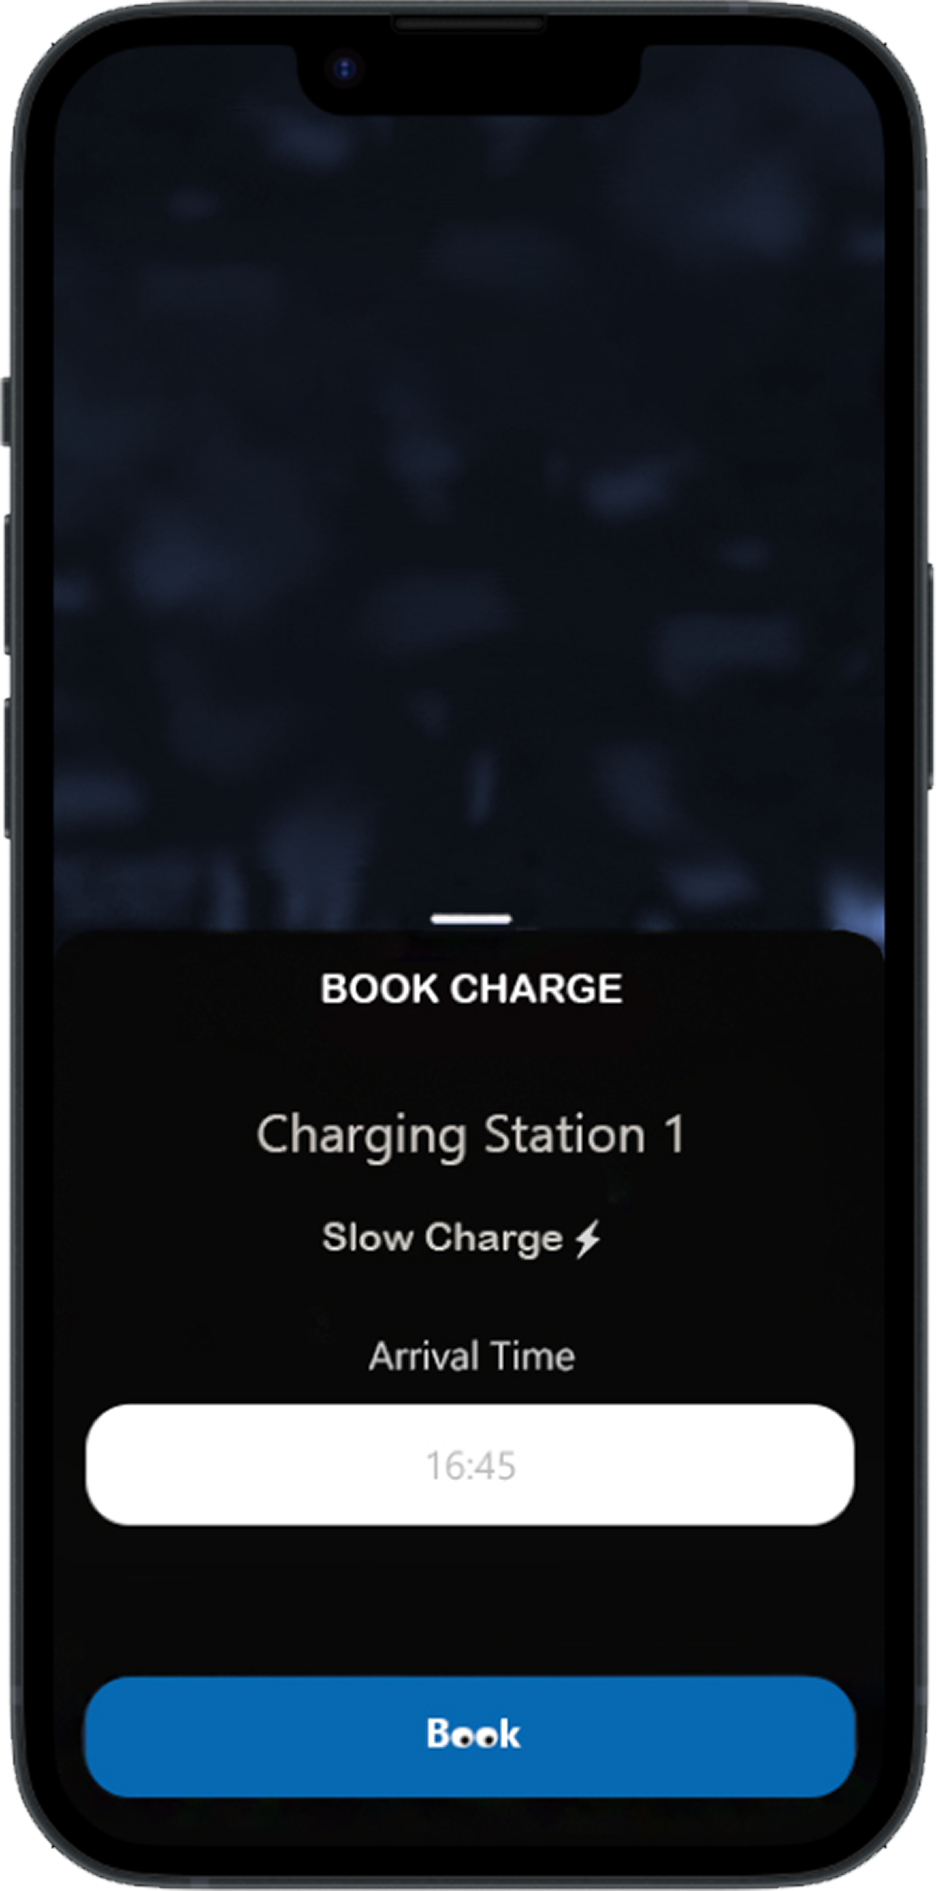
\includegraphics[
                width=\textwidth,
                height=\textheight,
                keepaspectratio]{SeqDia/BookCharge}
            \caption{Book a charging process}
            \label{fig:BookCharge}
            \end{center}
        \end{figure}
        \newpage
        \item \textbf{Delete Booking}
        \begin{figure}[H]
            \begin{center}
            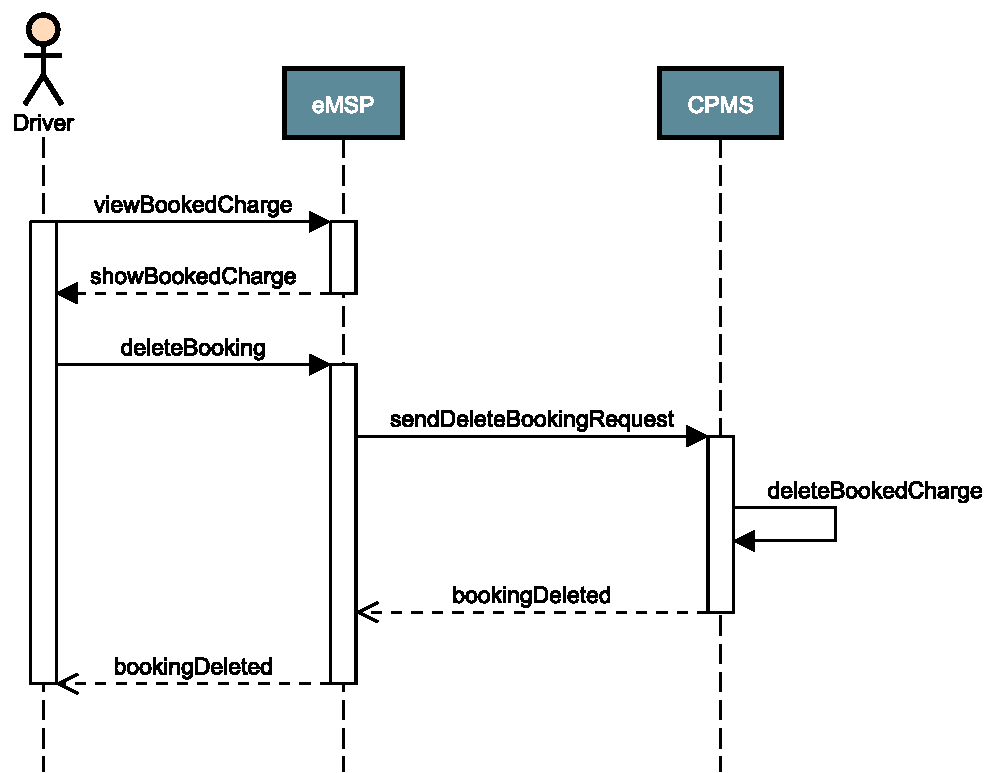
\includegraphics[
                width=\textwidth,
                height=0.6\textheight,
                keepaspectratio]{SeqDia/DeleteBooking}
            \caption{Delete a booked charging process}
            \label{fig:DeleteBooking}
            \end{center}
        \end{figure}
        \item \textbf{Suggestion Notification}
        \begin{figure}[H]
            \begin{center}
            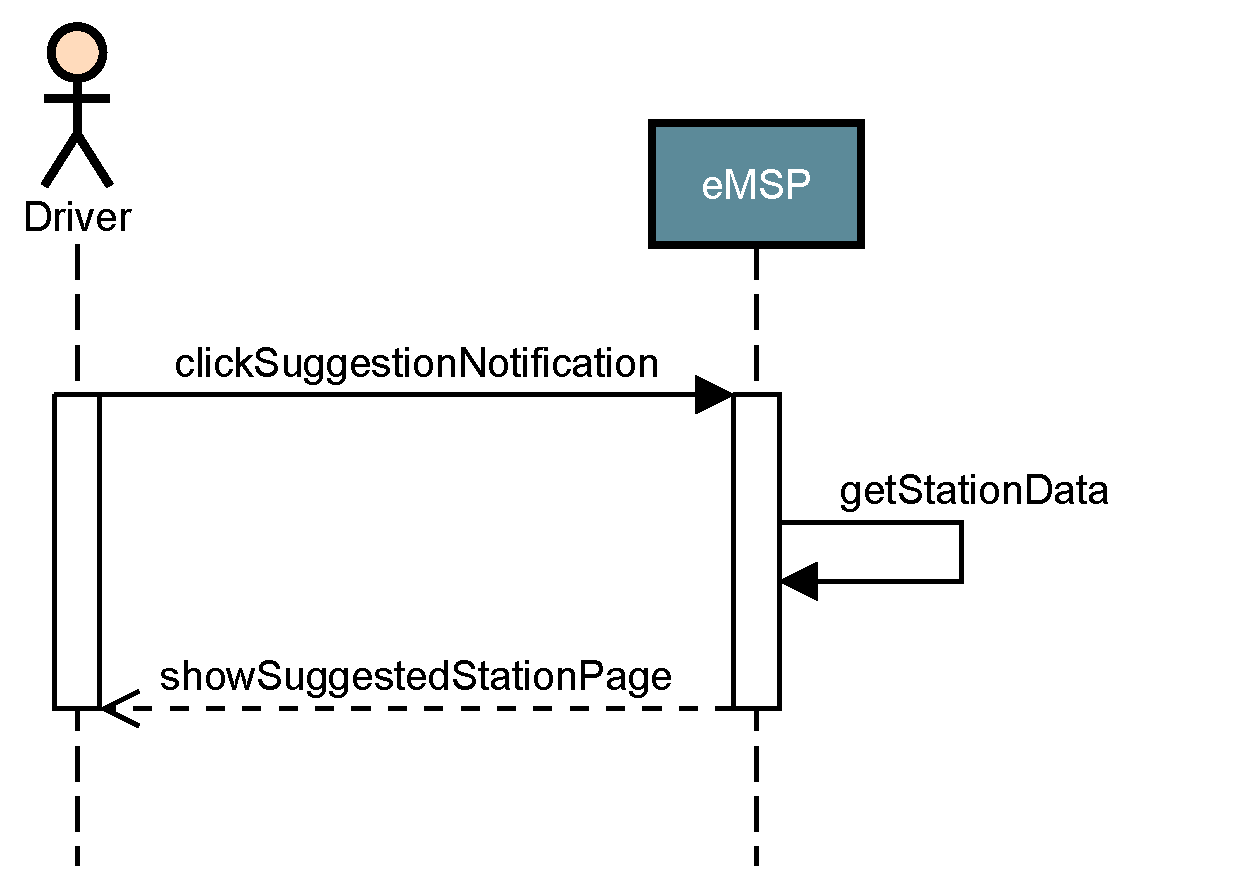
\includegraphics[
                width=\textwidth,
                height=0.3\textheight,
                keepaspectratio]{SeqDia/AdviceNotification}
            \caption{Driver receives and opens a suggestion}
            \label{fig:AdviceNotification}
            \end{center}
        \end{figure}
        \newpage
        \item \textbf{Charging Process}
        \begin{figure}[H]
            \begin{center}
            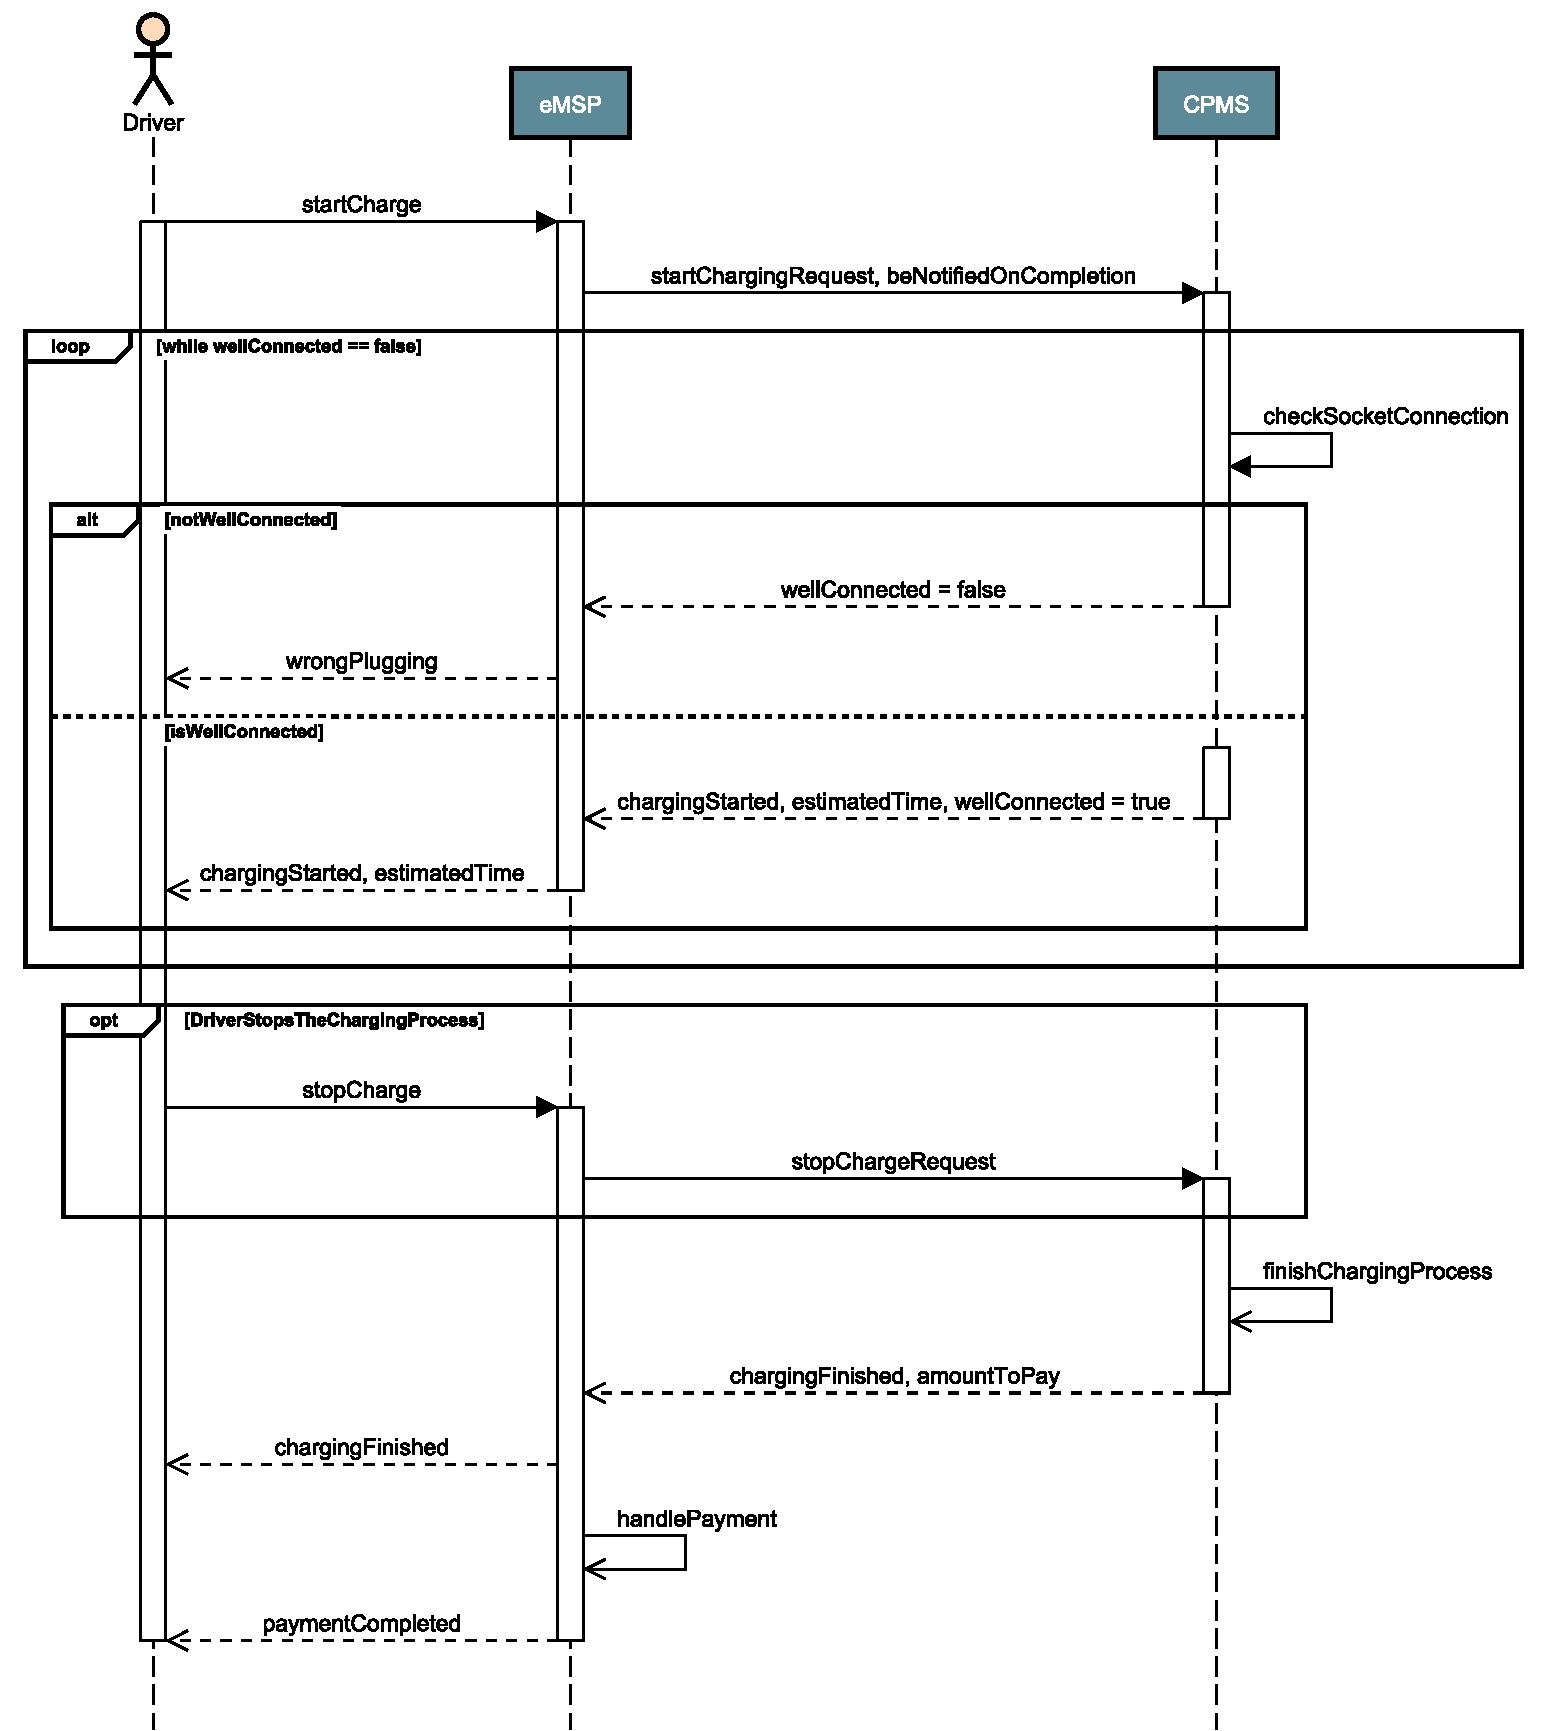
\includegraphics[
                width=\textwidth,
                height=\textheight,
                keepaspectratio]{SeqDia/StartCharge}
            \caption{Process of a charging process}
            \label{fig:StartCharge}
            \end{center}
        \end{figure}
        \newpage
        \item \textbf{CPO Login}
        \begin{figure}[H]
            \begin{center}
            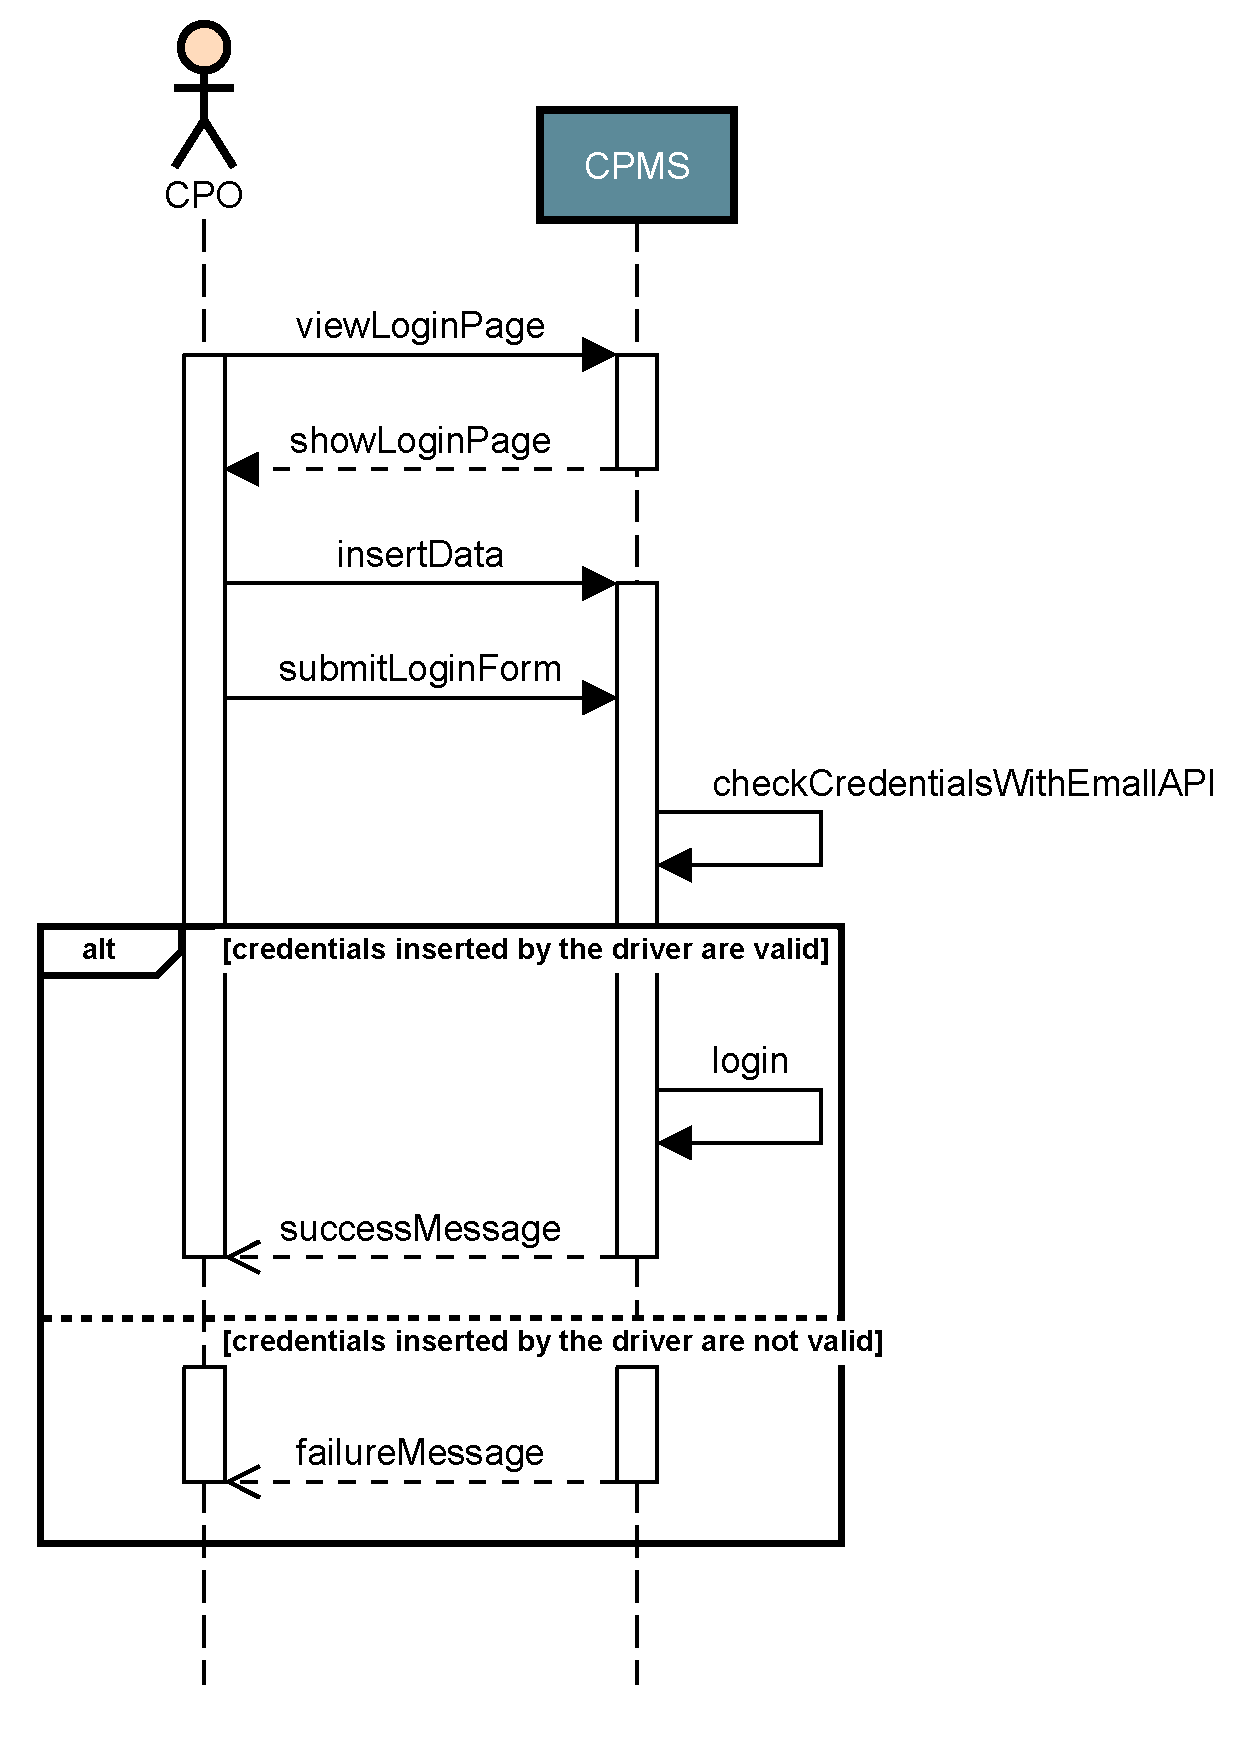
\includegraphics[
                width=\textwidth,
                height=0.45\textheight,
                keepaspectratio]{SeqDia/CPOLogin}
            \caption{Process of a charging process}
            \label{fig:CPOLogin}
            \end{center}
        \end{figure}
        \item \textbf{View Managed Station Status}
        \begin{figure}[H]
            \begin{center}
            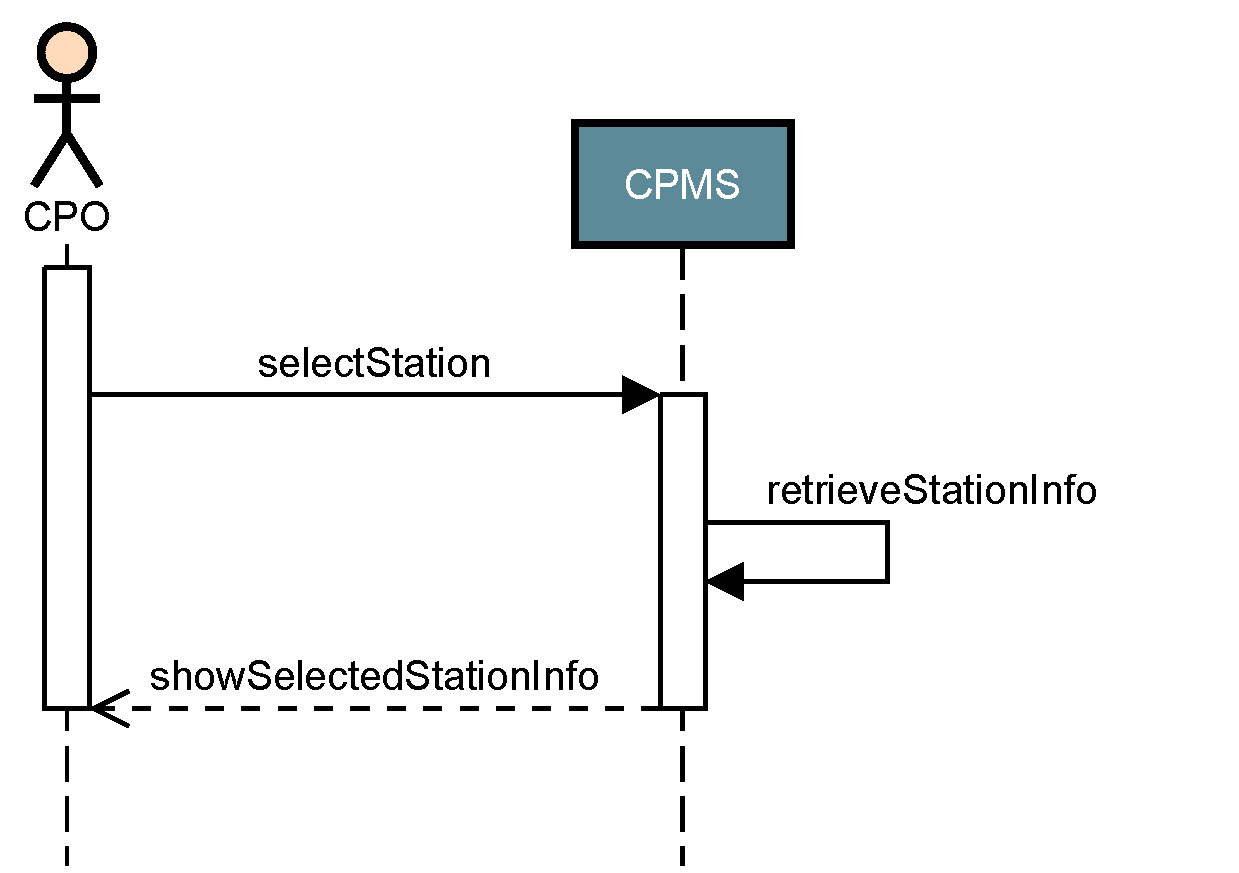
\includegraphics[
                width=\textwidth,
                height=0.35\textheight,
                keepaspectratio]{SeqDia/ManageStation}
            \caption{CPO views a managed station}
            \label{fig:ManageStation}
            \end{center}
        \end{figure}
        \newpage
        \item \textbf{Add Station To CPMS}
        \begin{figure}[H]
            \begin{center}
            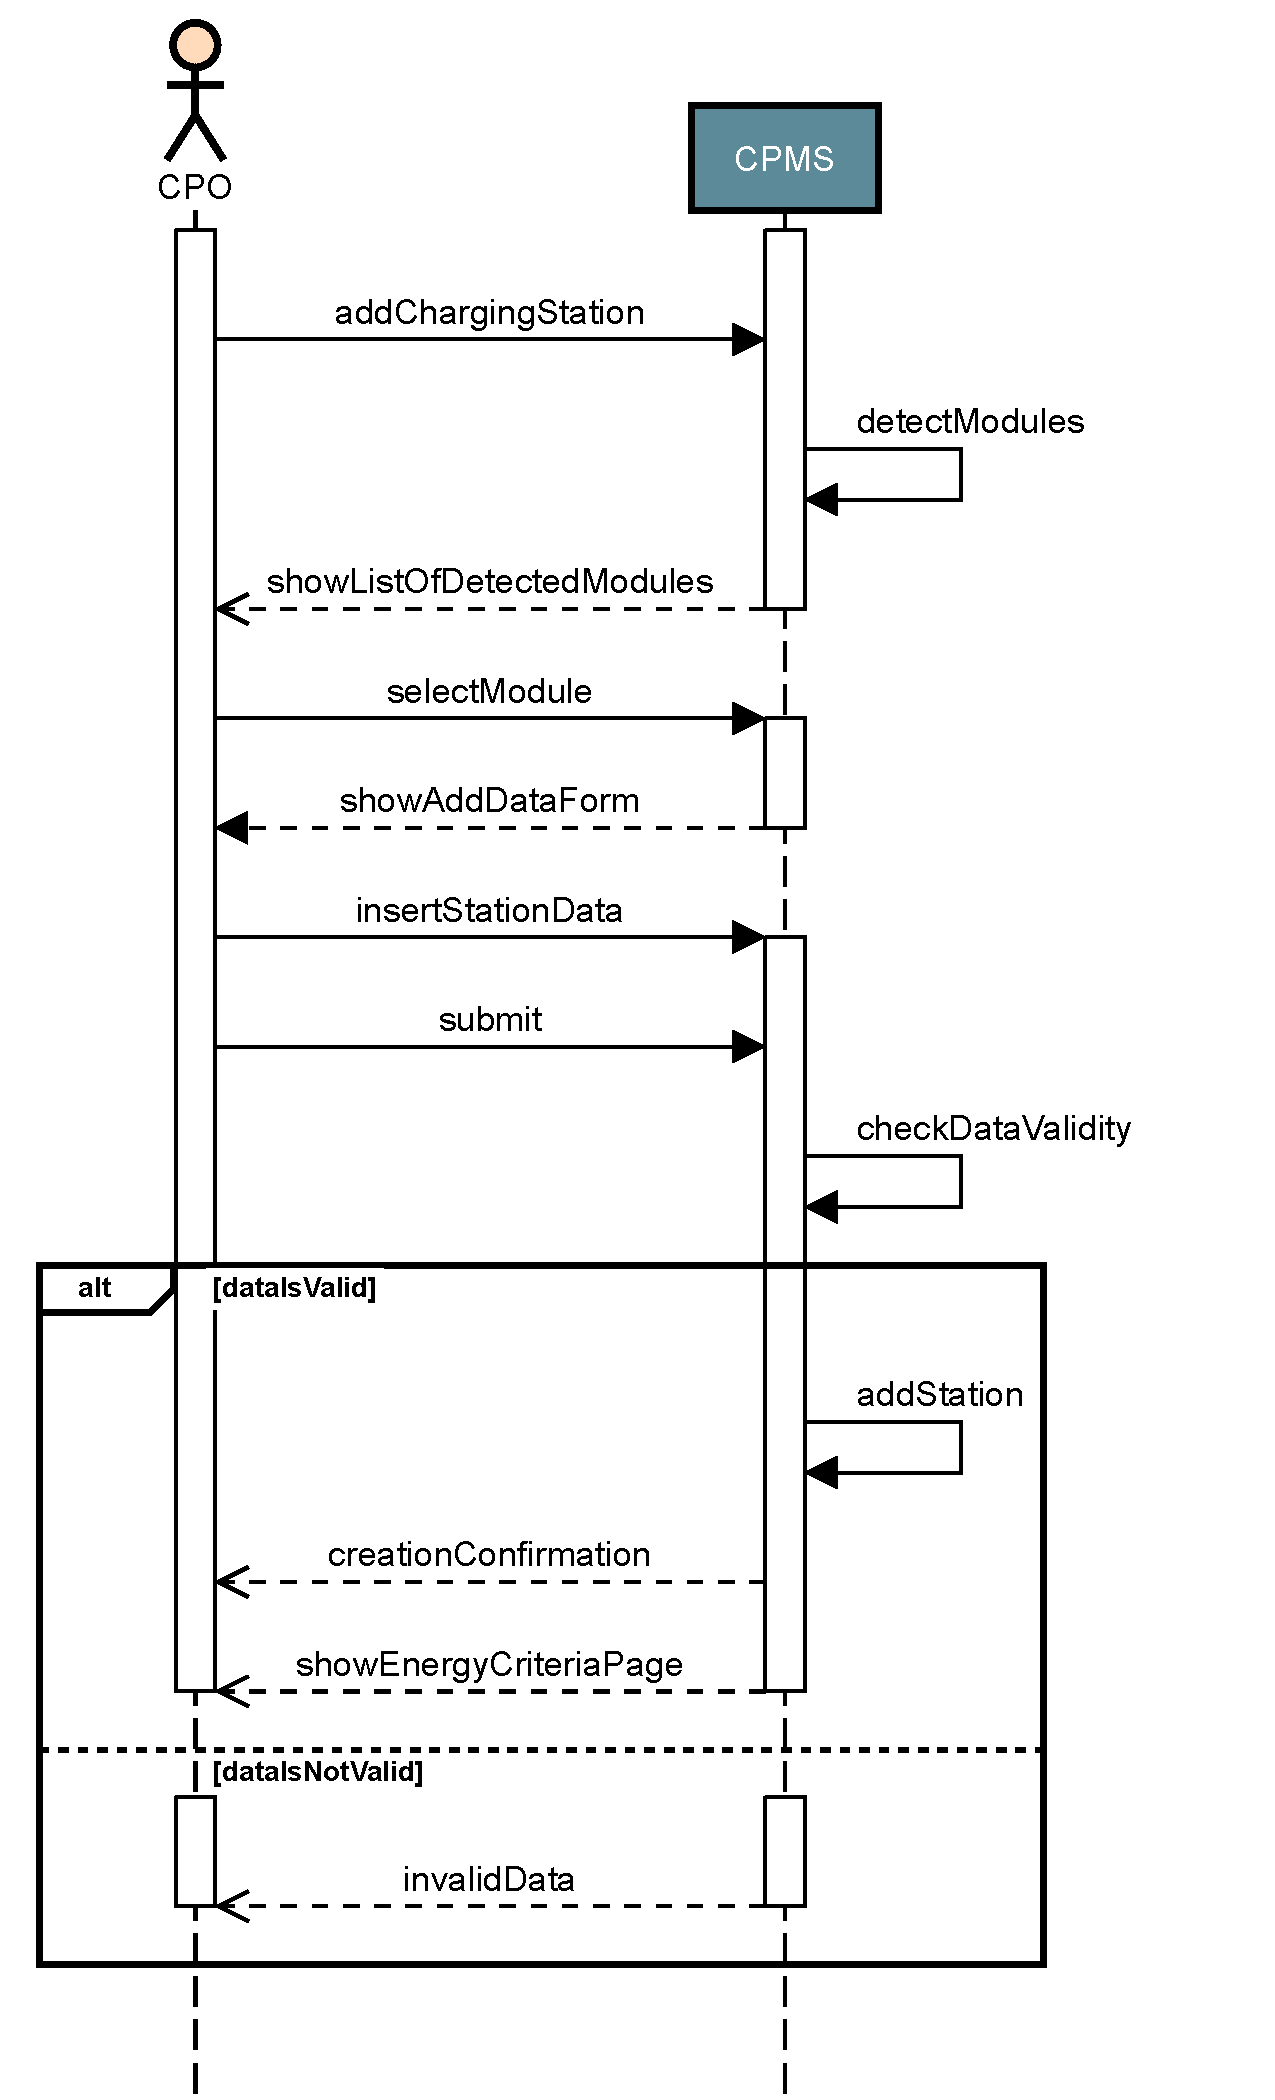
\includegraphics[
                width=\textwidth,
                height=0.85\textheight,
                keepaspectratio]{SeqDia/AddStation}
            \caption{CPO adds a station}
            \label{fig:AddStation}
            \end{center}
        \end{figure}
        \newpage
        \item \textbf{Set Offer}
        \begin{figure}[H]
            \begin{center}
            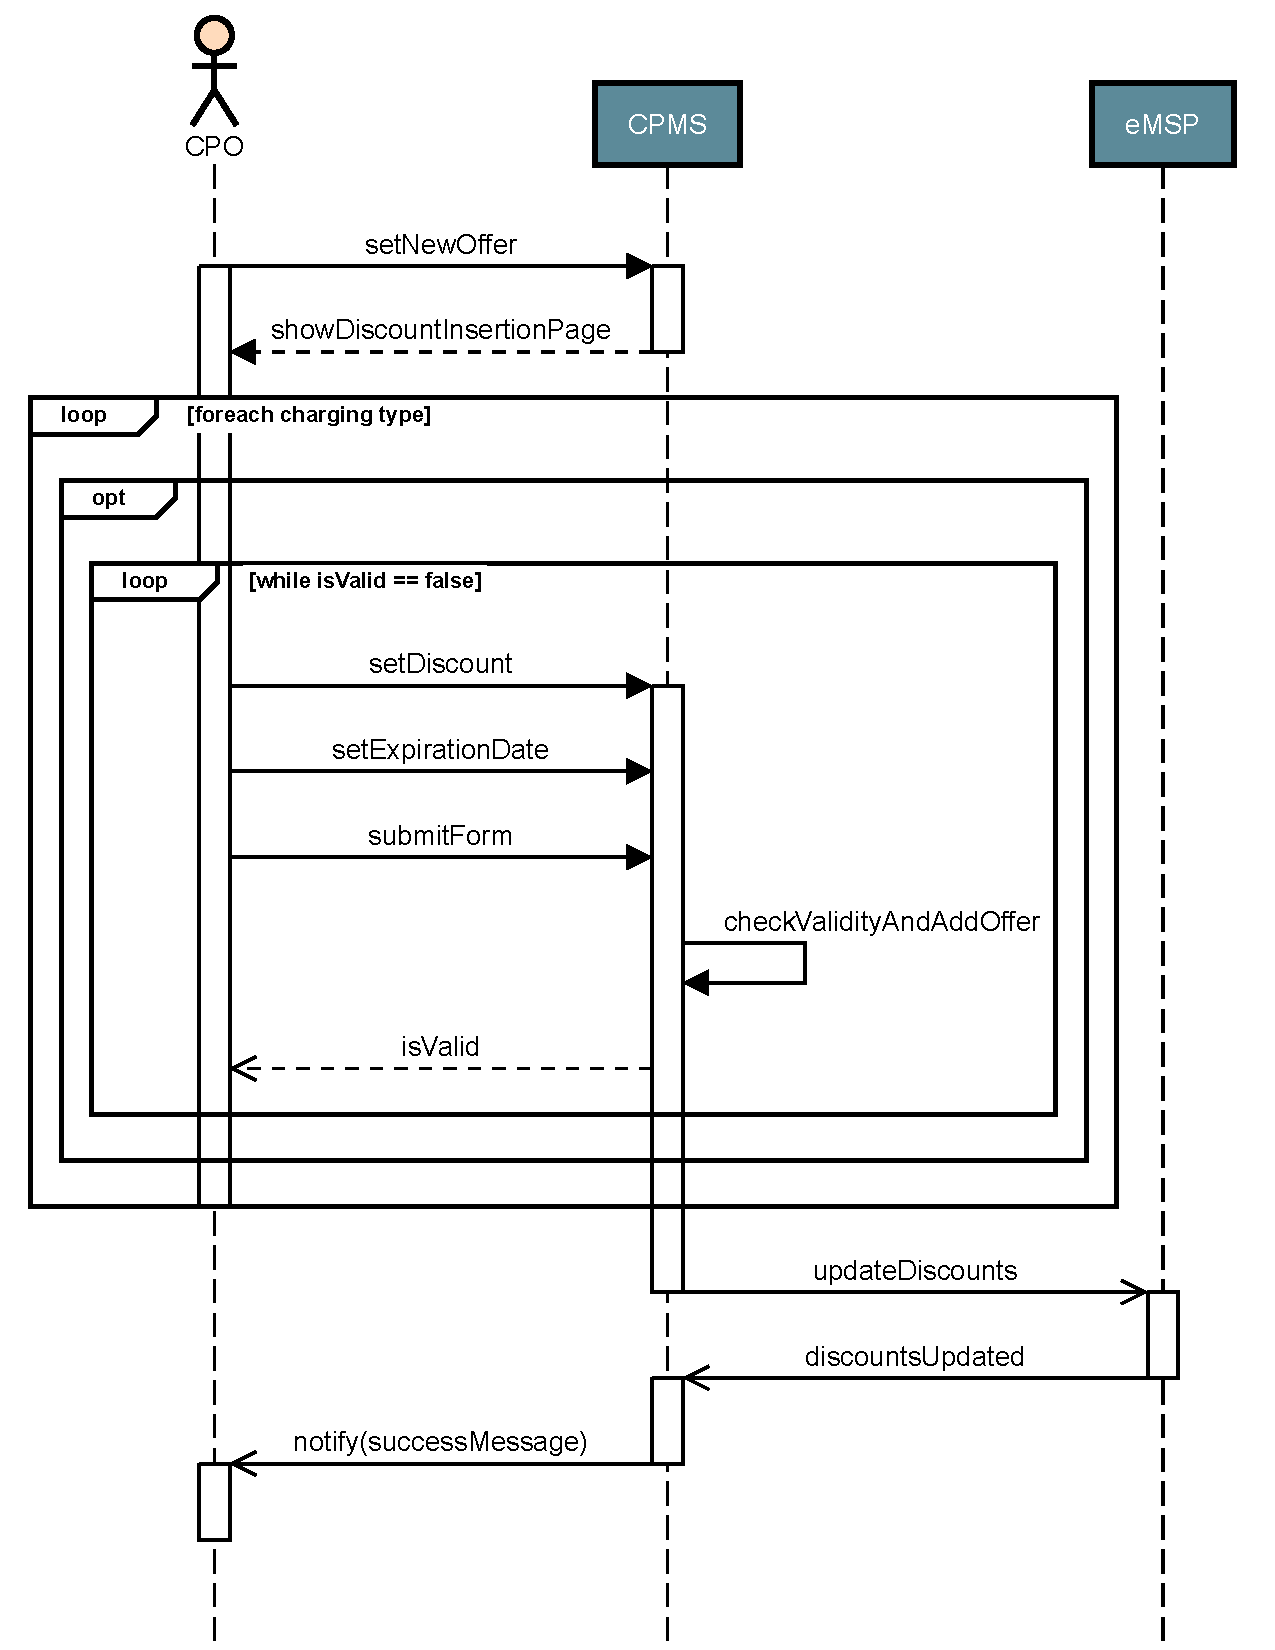
\includegraphics[
                width=\textwidth,
                height=\textheight,
                keepaspectratio]{SeqDia/SetOffer}
            \caption{CPO sets a new offer}
            \label{fig:SetOffer}
            \end{center}
        \end{figure}
        \newpage
        \item \textbf{Update Energy Criteria}
        \begin{figure}[H]
            \begin{center}
            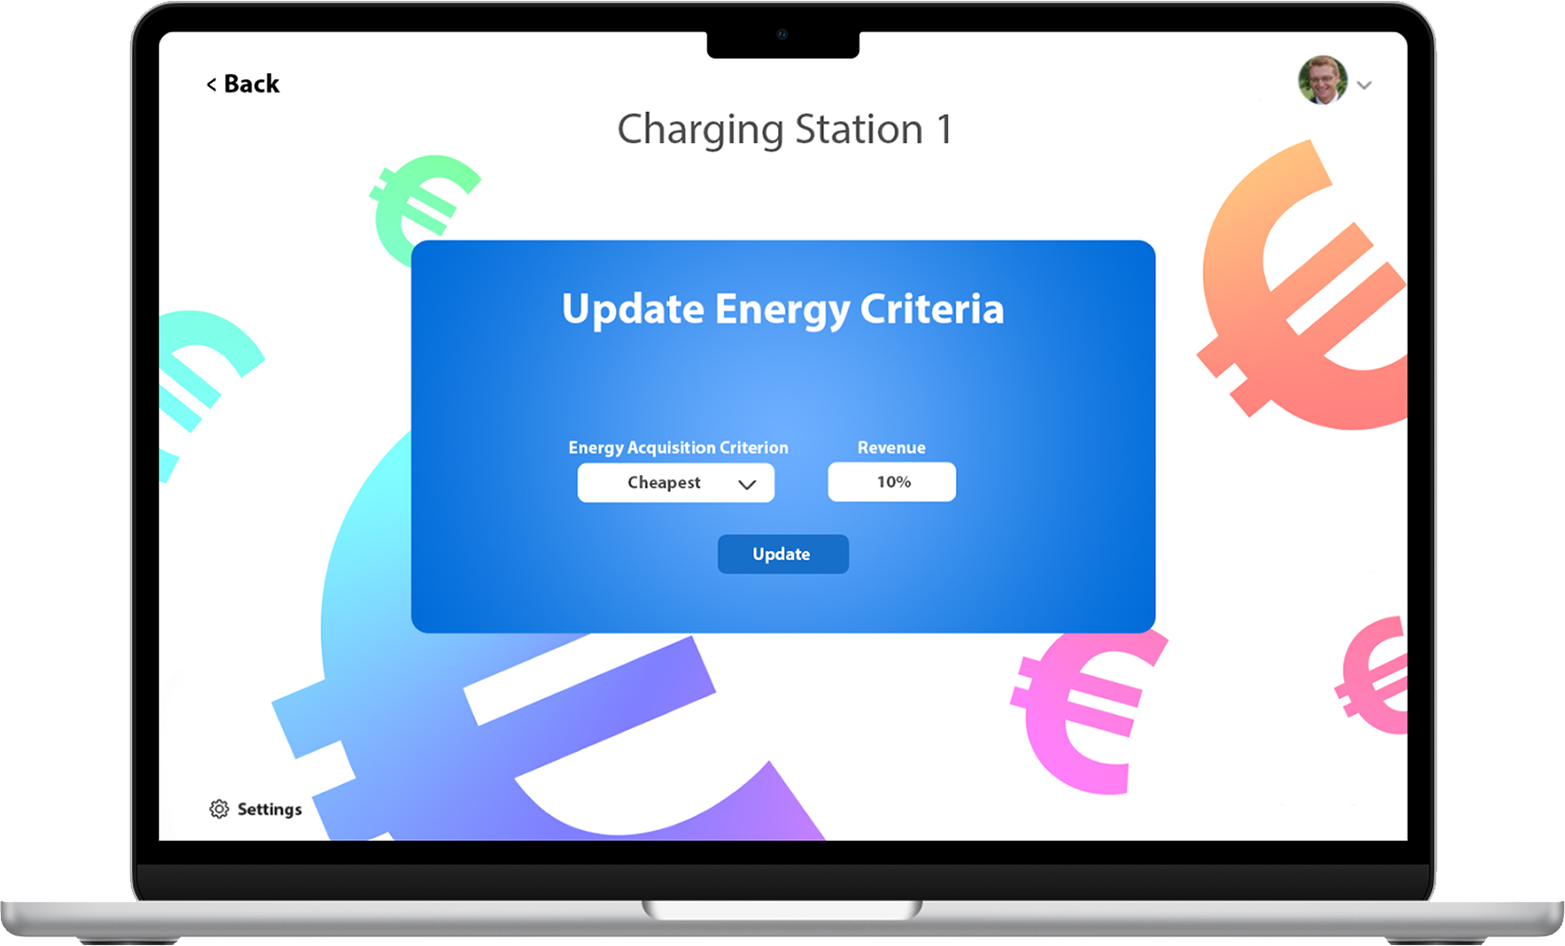
\includegraphics[
                width=\textwidth,
                height=0.85\textheight,
                keepaspectratio]{SeqDia/UpdateCriteria}
            \caption{CPO updates energy criteria}
            \label{fig:UpdateCriteria}
            \end{center}
        \end{figure}
        \newpage
        \item \textbf{eMSP Association}
        \begin{tabbing}
            \textbf{Note}: \= In \textit{sendCPOData} is also passed a payment method where the associated eMSP\\
            \> will send future drivers' payments.
        \end{tabbing}
        \begin{figure}[H]
            \begin{center}
            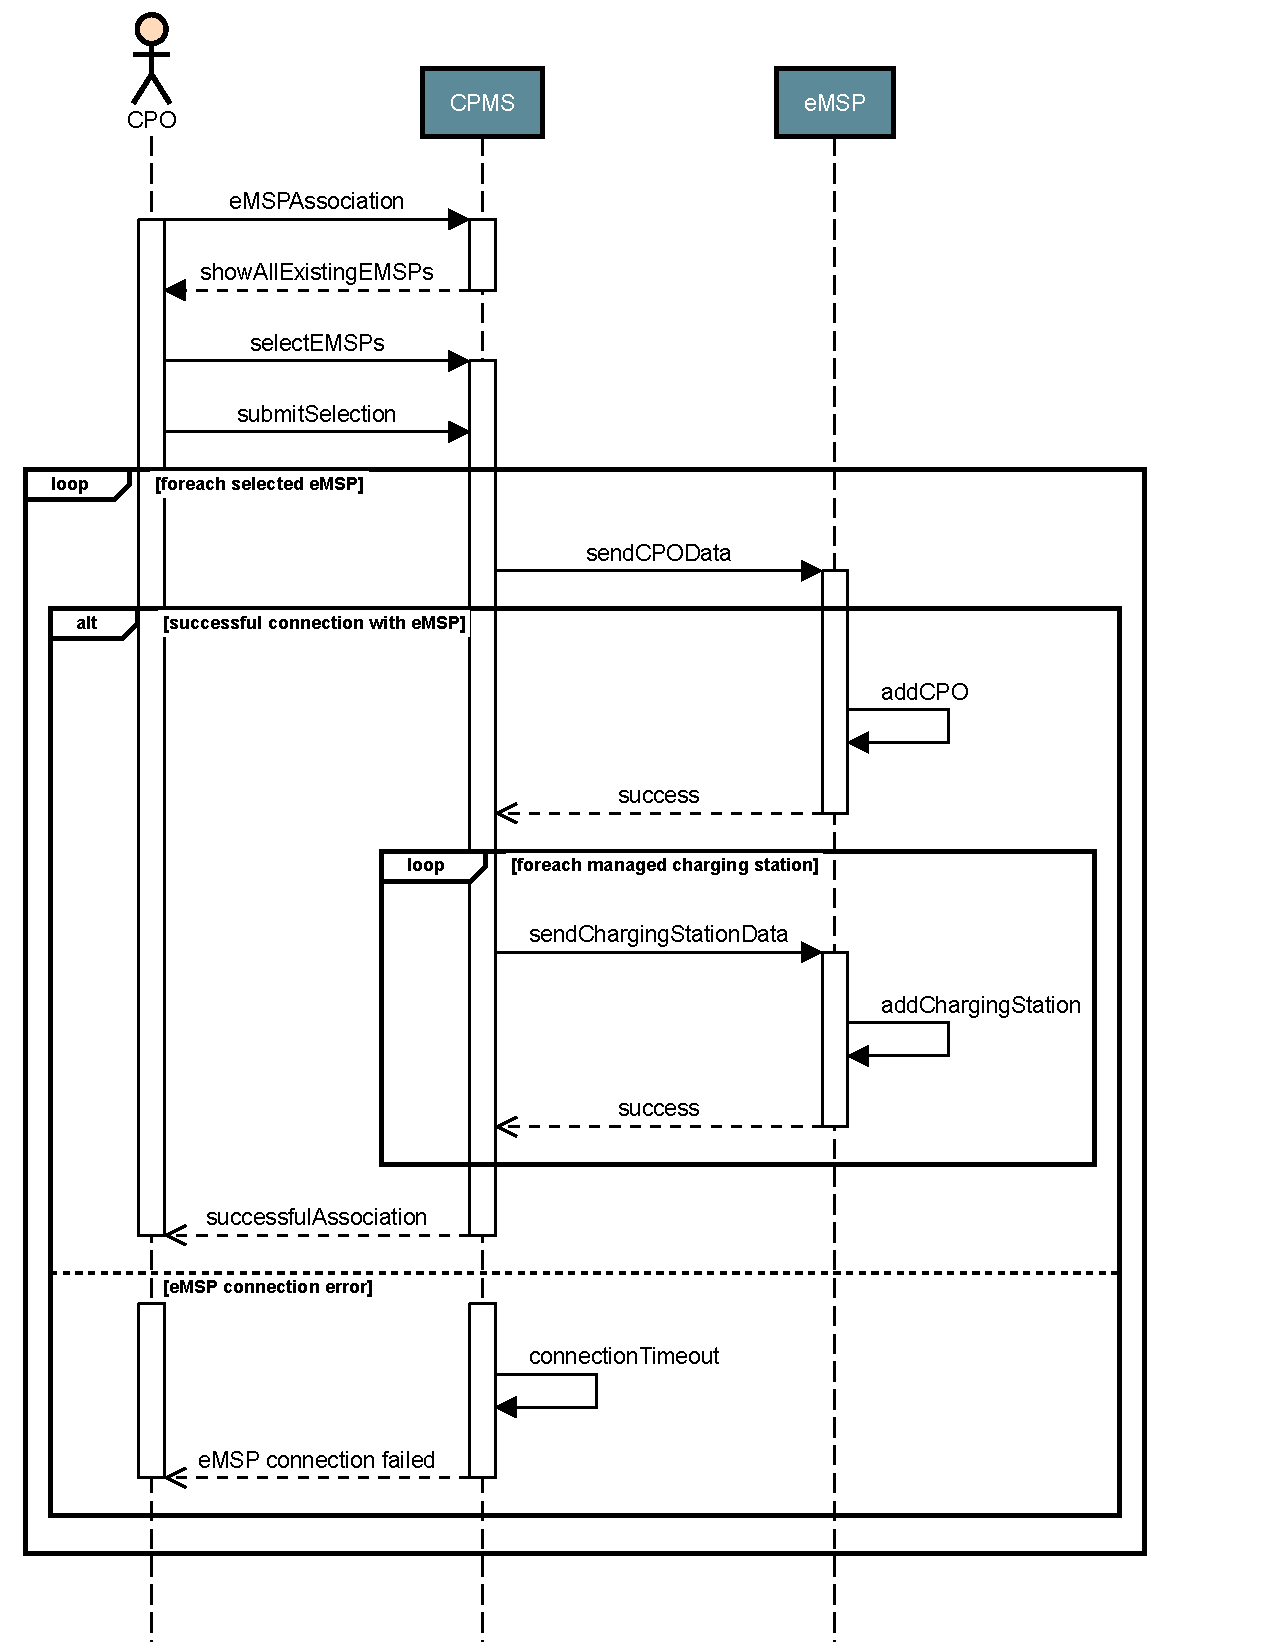
\includegraphics[   
                width=\textwidth,
                height=0.85\textheight,
                keepaspectratio]{SeqDia/eMSPAssociation}
            \caption{CPO associates a new eMSP}
            \label{fig:eMSPAssociation}
            \end{center}
        \end{figure}
\end{enumerate}
\restoregeometry
\subsection{eMSP Requirements}
In this section, the requirements for the two subsystems will be described as also their interactions. For both the Drivers and the CPOs it is required to be logged in to the system in order to perform any action different from Login and Registration
\begin{longtable}
{| p{0.12\linewidth} |p{0.28\linewidth} | p{0.6\linewidth} |}
    \hline
    \rowcolor{bluepoli!40}
     \textbf{ID} & \textbf{Name}& \textbf{Description} \T\B \\
    \hline 
    \hline
    \textbf{FRE\row} & Driver Registration & An Unregistered Driver shall be able to register himself on the eMSP application.\T\B\\
    \hline
    \textbf{FRE\row} & Driver Login &The Driver shall be able to login to the eMSP with his credentials.\T\B\\
    \hline
    \textbf{FRE\row} & Internet Connection & The system shall notify the Driver if there is no internet connection.\T\B\\
    \hline
    \textbf{FRE\row} & View Charging Stations & The Driver shall be able to see the location of all the charging stations in a certain geographic area.\T\B\\
    \hline
    \textbf{FRE\row} & Charging Type Selection & The Driver shall be able to select the charging types he is interested in while searching for a charging station in order to filter them.\T\B\\
    \hline
    \textbf{FRE\row} & Charging Cost & The Driver shall be able to check the cost per kWh for the specified charging types in a specific charging station.\T\B\\
    \hline
    \textbf{FRE\row} & Charging Station Availability & The Driver shall be able to see which charging stations are currently available for the specified charging types.\T\B\\
    \hline
    \textbf{FRE\row} & Future Availability & The Driver shall be able to see an estimated time in which a specific charging station will become available.\T\B\\
    \hline
    \textbf{FRE\row} & Charge Booking & The Driver shall be able to book a charging socket in an available charging station, from 0 up to a max specified amount of time before.\T\B\\
    \hline
    \textbf{FRE\row} & Booked Charging Socket ID & The system shall show the Driver the booked socket ID number.\T\B\\
    \hline
    \textbf{FRE\row} & Delete Booking & The Driver shall be able to delete a booked charging process before its starting time.\T\B\\
    \hline
    \textbf{FRE\row} & Confirm Booking & The Driver shall receive a notification that confirms the booking went well.\T\B\\
    \hline
    \textbf{FRE\row} & Start Charging Process & As soon as the booked time starts the Driver shall be able to start the recharging process.\T\B\\
    \hline
    \textbf{FRE\row} & Stop Charging Process & During the recharging process the Driver shall be able to stop it in advance.\T\B\\
    \hline
    \textbf{FRE\row} & Time remaining  & The Driver shall be able to check the estimated remaining time until the end of the charging process.\T\B\\
    \hline
    \textbf{FRE\row} & Charge Finished  & The system shall notify the Driver when the charging process is complete.\T\B\\
    \hline
    \textbf{FRE\row} & Payment & At the end of the charging process, the system shall handle the payment between the Driver and the CPO through an external API.\T\B\\%, retrieving from the Driver’s given payment method the amount of money to pay requested by the CPMS for that charge.\T\B\\
    \hline   
    \textbf{FRE\row} & Generic Error Notification & Every time the system fails to elaborate an operation related to a Driver, then he shall receive a notification containing the error details.\T\B\\
    \hline
    \textbf{FRE\row} & Successful Payment Notification & The system shall notify the Driver when a successful payment occurs.\T\B\\
    \hline    
    \textbf{FRE\row} & Check Vehicle Connection & The system shall be able to check if there exists a connection between the Driver's vehicle and the system itself.\T\B\\
    \hline
    \textbf{FRE\row} & Vehicle’s Remaining Charge & If the vehicle is connected, the system shall be able to retrieve the battery level of the Driver's vehicle.\T\B\\
    \hline
    \textbf{FRE\row} & Vehicle’s Location & If the vehicle is connected, the system shall be able to retrieve the Driver's vehicle location.\T\B\\
    \hline
    \textbf{FRE\row} & Data Integration & The Driver shall be able to authorize the system to access his personal data such as his calendar, navigation system and location.\T\B\\
    \hline
    \textbf{FRE\row} & Calendar Data & The system shall be able to retrieve data from the Driver's personal calendar.\T\B\\
    \hline
    \textbf{FRE\row} & Navigation System & The system shall retrieve information about the Driver’s navigation system.\T\B\\
    \hline
    \textbf{FRE\row} & Charging Suggestion Creation & If the vehicle is connected to the Driver's device, the eMSP shall create charging suggestion notifications based on the status of the vehicle's battery, the Driver's schedule (his calendar and navigation system), special offers made available at some charging stations and the availability of charging sockets at those identified charging stations.\T\B\\
    \hline
    \textbf{FRE\row} & Suggestion Notification & The system shall advise the Driver with a notification when and where he should recharge his vehicle’s battery.\T\B\\
    \hline    
    \textbf{FRE\row} & Suggestion Interaction & The Driver shall be able to click on the charging suggestion notification sent by the eMSP and that shall redirect to the suggested charging station's info page.\T\B\\
    \hline
    %\textbf{FRE\row} & CPMS communication & The system shall be able to communicate with the specific CPMS while performing an operation within one of its managed stations. \T\B\\
    %\hline
    \caption{Table of eMSP Requirements}
\end{longtable}
\subsection{CPMS Requirements}
\begin{longtable}{| p{0.12\linewidth} |p{0.28\linewidth} | p{0.6\linewidth} |}
    \hline
    \rowcolor{bluepoli!40}
     \textbf{ID} & \textbf{Name}& \textbf{Description} \T\B \\
    \hline 
    \hline
    \textbf{FRE\row} & CPO Login & The CPO shall be able to login to the CPMS with his credentials.\T\B\\
    \hline
    \textbf{FRE\row} & Internet Connection & The system shall notify the CPO if there is no internet connection.\T\B\\
    \hline
    \textbf{FRE\row} & View Charging Stations & The CPO shall be able to see the list of only all his owned charging stations.\T\B\\
    \hline
    \textbf{FRE\row} & Add Charging Station & The CPO shall be able to add a new charging station.\T\B\\
    \hline
    \textbf{FRE\row} & Batteries Energy & The CPO shall be able to check the remaining energy stored in the batteries in one of his own charging stations.\T\B\\
    \hline
    \textbf{FRE\row} & Number Of Vehicles  & The CPO shall be able to check the number of vehicles being charged in one of his charging stations.\T\B\\
    \hline
    \textbf{FRE\row} & Power Absorption  & The CPO shall be able to check the amount of power absorbed from each vehicle being charged in one of his charging stations.\T\B\\
    \hline
    \textbf{FRE\row} & Charging Time Left  & The system shall be able to give an estimation about how much time is needed to end the charging process for a particular vehicle being charged in a charging station.\T\B\\
    \hline
    \textbf{FRE\row} & Energy Price Information & The system shall be able to retrieve the current energy price and the capacity for each of the available DSOs.\T\B\\
    \hline   
    \textbf{FRE\row} & Battery Energy Provider & The system shall be able to use the batteries as energy providers with prices equal to the cost that was used to recharge them. \T\B\\
    \hline
    \textbf{FRE\row} & Energy Acquisition Criteria & The CPO shall be able to select the criteria that will be used by the CPMS in order to acquire energy, such as Energy provider with the lowest price, Energy Provider with biggest energy capacity.\T\B\\
    \hline
    \textbf{FRE\row} & Energy Revenue Criteria  & The CPO shall be able to select the revenue percentage amount from the energy sale of each charging station.\T\B\\
    \hline
    \textbf{FRE\row} & Energy Acquisition Decision & The system shall be able, for each charging station, to automatically decide from which energy provider to retrieve the energy, based on the criteria chosen by the CPO.\T\B\\
    \hline
    \textbf{FRE\row} & Energy Sale Price  & The system shall be able, for each charging station, to automatically calculate the selling price of the energy based on the revenue criteria and on the price of the energy provider.\T\B\\
    \hline 
    \textbf{FRE\row} & Payment Calculation & The system shall be able to calculate when a charging process ends, the amount requested to pay based on the energy consumed and its selling price.\T\B\\
    \hline 
    \textbf{FRE\row} & Internal Battery Management & The system shall be able to automatically decide whether to store or not energy in the internal batteries, if available, of one of the managed charging stations.\T\B\\
    \hline
    \textbf{FRE\row} & Special Offers  & The system shall allow the CPO to apply discounts for the energy prices of a managed charging station until a set expiration date.\T\B\\
    \hline
    \textbf{FRE\row} & eMSP List & The CPO shall be able to see a list of all the existing eMSPs.\T\B\\
    \hline
    \textbf{FRE\row}& eMSP Association & The CPO shall be able to decide which eMSP he wants to associate with his CPMS in order to permit communication between the two systems. \T\B\\
    \hline
    \caption{Table of CPMS Requirements}
\end{longtable}
\subsection{Interaction Requirement}
Here there is the description of the requirements that are in common between the two subsystems. To avoid having a large number of requirements, the following ones should be read in this way:\\
\begin{itemize}
    \item\textbf{Format 1}: The eMSP shall (be able to) "perform an operation" on a single CPMS:
    \begin{itemize}
        \item The eMSP shall communicate with the CMPS requesting to "perform an operation".
        \item The CPMS shall return to eMSP the result of the "performed operation".
    \end{itemize}
    \item \textbf{Format 2}: CPMS updates "data":
    \begin{itemize}
        \item The CPMS shall detect when some "data" is updated.
        \item The CPMS shall send to every associated eMSP the new updated "data".
        \item The eMSP shall store the "data" received by the CMPS and show it to the driver when he requests it.
    \end{itemize}
\end{itemize}
\begin{longtable}{| p{0.12\linewidth} |p{0.28\linewidth} | p{0.6\linewidth} |}
    \hline
    \rowcolor{bluepoli!40}
     \textbf{ID} & \textbf{Name}& \textbf{Description} \T\B \\
    \hline 
    \hline
    \textbf{FRE\row} & Book a charge & The eMSP shall be able to book a charge and receive the booked charging socket on a single CPMS.\T\B\\
    \hline
    \textbf{FRE\row} & Delete a booked charge & The eMSP shall be able to delete a previously booked charge on a single CPMS.\T\B\\
    \hline
    \textbf{FRE\row} & Start charge & The eMSP shall be able to start a charge on a single CPMS.\T\B\\
    \hline
    \textbf{FRE\row} & Wrong plugging & The eMSP shall be notified when the vehicle is not well connected to the charging socket on a single CPMS.\T\B\\
    \hline 
    \textbf{FRE\row} & Stop charge & The eMSP shall be able to stop a charge on a single CPMS.\T\B\\
    \hline
    \textbf{FRE\row} & Amount to pay & The eMSP shall be notified with the required amount of money to pay when the charging process ends on a single CPMS .\T\B\\
    \hline
    \textbf{FRE\row} & Remaining Charge Time & The eMSP shall be able to ask for the estimated ending time for a specific charging process.\T\B\\
    \hline
    \textbf{FRE\row}& Charging station availability & If CPMS can calculate the estimated time before each charging type becomes available, CPMS updates the availability of a charging station with the estimated time otherwise, CPMS updates only the availability. \T\B\\
    \hline
    \textbf{FRE\row}& Charging station price & CPMS updates the price of a charging type in a station.\T\B\\
    \hline
    \textbf{FRE\row} &Charging station offer & CPMS updates the offer of a charging type in a station.\T\B\\
    \hline
    \textbf{FRE\row} & Charging station creation & CPMS updates about the data of the newly created charging station such as location, prices, supported charging types.\T\B\\
    \hline
    \caption{Table of Interaction Requirements}
    \setcounter{row}{0}
\end{longtable}
\newpage
\subsection{Requirements mapping on Goals}
\begin{longtable}{| p{0.1\linewidth} | P{0.05\linewidth} |P{0.05\linewidth} |P{0.05\linewidth} |P{0.05\linewidth} |P{0.05\linewidth} |P{0.05\linewidth} | P{0.05\linewidth}|}
    \hline
    \rowcolor{bluepoli!40}
     \textbf{R/G} & \textbf{G1} & \textbf{G2}& \textbf{G3}& \textbf{G4}& \textbf{G5}& \textbf{G6} &\textbf{G7}\T\B \\
    \hline 
    \hline
    \textbf{FRE\row} &X &X &X &X & & &\T\B\\
    \hline
    \textbf{FRE\row} &X &X &X &X & & &\T\B\\
    \hline
    \textbf{FRE\row} &X &X &X &X & & &\T\B\\
    \hline
    \textbf{FRE\row} &X &X & & & & &\T\B\\
    \hline
    \textbf{FRE\row} &X &X & & & & &\T\B\\
    \hline
    \textbf{FRE\row} &X & & & & & &\T\B\\
    \hline
    \textbf{FRE\row} &X &X & & & & &\T\B\\
    \hline
    \textbf{FRE\row} &X &X & & & & &\T\B\\
    \hline
    \textbf{FRE\row} & &X & & & & &\T\B\\
    \hline
    \textbf{FRE\row} & &X &X & & & & \T\B\\
    \hline
    \textbf{FRE\row} & &X & & & & &\T\B\\
    \hline
    \textbf{FRE\row} & &X & & & & &\T\B\\
    \hline
    \textbf{FRE\row} & & &X & & & &\T\B\\
    \hline
    \textbf{FRE\row} & & &X & & & &\T\B\\
    \hline
    \textbf{FRE\row} & & &X & & & &\T\B\\
    \hline
    \textbf{FRE\row} & & &X & & & &\T\B\\
    \hline
    \textbf{FRE\row} & & & &X & & & \T\B\\
    \hline
    \textbf{FRE\row} &X &X &X &X &X & & \T\B\\
    \hline
    \textbf{FRE\row} & & & &X & & & \T\B\\
    \hline
    \textbf{FRE\row} & & & & &X & & \T\B\\
    \hline
    \textbf{FRE\row} & & & & &X & & \T\B\\
    \hline
    \textbf{FRE\row} &X & & & &X & & \T\B\\
    \hline
    \textbf{FRE\row} & & & & &X & & \T\B\\
    \hline
    \textbf{FRE\row} & & & & &X & & \T\B\\
    \hline
    \textbf{FRE\row} & & & & &X & & \T\B\\
    \hline
    \textbf{FRE\row} & & & & &X & & \T\B\\
    \hline
    \textbf{FRE\row} & & & & &X & & \T\B\\
    \hline
    \textbf{FRE\row} & & & & &X & & \T\B\\
    \hline
    \hhline{========}
    \textbf{FRE\row} & & & & & &X &X\T\B\\
    \hline
    \textbf{FRE\row} & & & & & &X &X\T\B\\
    \hline
    \textbf{FRE\row} & & & & & &X &X\T\B\\
    \hline
    \textbf{FRE\row} & & & & & &X &X\T\B\\
    \hline
    \textbf{FRE\row} & & & & & & &X\T\B\\
    \hline
    \textbf{FRE\row} & & & & & & &X\T\B\\
    \hline
    \textbf{FRE\row} & & & & & & &X\T\B\\
    \hline
    \textbf{FRE\row} & & &X & & & &X\T\B\\
    \hline
    \textbf{FRE\row} & & & & & &X &\T\B\\
    \hline
    \textbf{FRE\row} & & & & & &X &\T\B\\
    \hline
    \textbf{FRE\row} & & & & & &X &\T\B\\
    \hline
    \textbf{FRE\row} & & & &X& &X &\T\B\\
    \hline
    \textbf{FRE\row} & & & & & &X &\T\B\\
    \hline
    \textbf{FRE\row} & & & &X& &X &\T\B\\
    \hline
    \textbf{FRE\row} & & & &X & & &\T\B\\
    \hline
    \textbf{FRE\row} & & & & & &X &\T\B\\
    \hline
    \textbf{FRE\row} &X & & & &X &X &\T\B\\
    \hline
    \textbf{FRE\row} &X &X &X &X &X & &\T\B\\
    \hline
    \textbf{FRE\row} &X &X &X &X &X& &\T\B\\
    \hhline{========}
    \textbf{FRE\row} & &X & & & & &\T\B\\
    \hline
    \textbf{FRE\row} & &X & & & & &\T\B\\
    \hline
    \textbf{FRE\row} & & &X & & & &X\T\B\\
    \hline
    \textbf{FRE\row} & & &X & & & &\T\B\\
    \hline
    \textbf{FRE\row} & & &X & & & &X\T\B\\
    \hline
    \textbf{FRE\row} & & &X &X & & &\T\B\\
    \hline
    \textbf{FRE\row} & & &X & & & &X\T\B\\
    \hline
    \textbf{FRE\row} &X &X & & &X & &\T\B\\
    \hline
    \textbf{FRE\row} &X & & & &X & &\T\B\\
    \hline
    \textbf{FRE\row} &X & & & &X & &\T\B\\
    \hline
    \textbf{FRE\row} &X &X & & &X & &\T\B\\
    \hline
    \caption{Mapping of Requirements on Goals}
    \setcounter{row}{0}
\end{longtable}
\newpage
\subsection{Domain Assumption mapping on Goals}
\begin{longtable}{| p{0.1\linewidth} | P{0.05\linewidth} |P{0.05\linewidth} |P{0.05\linewidth} |P{0.05\linewidth} |P{0.05\linewidth} |P{0.05\linewidth} | P{0.05\linewidth}|}
    \hline
    \rowcolor{bluepoli!40}
     \textbf{R/G} & \textbf{G1} & \textbf{G2}& \textbf{G3}& \textbf{G4}& \textbf{G5}& \textbf{G6} &\textbf{G7}\T\B \\
    \hline 
    \hline
    \textbf{D\row} & & &X & & & &\T\B\\
    \hline
    \textbf{D\row} &X &X &X &X &X & &\T\B\\
    \hline
    \textbf{D\row} &X & &X & & & &\T\B\\
    \hline
    \textbf{D\row} & &X &X & & & &\T\B\\
    \hline
    \textbf{D\row} & X & X & X & & & &\T\B\\
    \hline
    \textbf{D\row} & & &X & & & &\T\B\\
    \hline
    \textbf{D\row} & & &X && & &\T\B\\
    \hline
    \textbf{D\row} & &X &X & & & &\T\B\\
    \hline
    \textbf{D\row} & & & & &X & &\T\B\\
    \hline
    \textbf{D\row} & & & & & X & & \T\B\\
    \hline
    \textbf{D\row} & & & & & & X &X\T\B\\
    \hline
    \textbf{D\row} & & & & & & X &\T\B\\
    \hline
    \textbf{D\row} & & & & X& &  &\T\B\\
    \hline
    \textbf{D\row} &X & & & & & &\T\B\\
    \hline
    \textbf{D\row} &X &X &X &X &X & &\T\B\\
    \hline
    \textbf{D\row} & & & & & &X &X\T\B\\
    \hline
    \caption{Mapping of Domain Assumptions on Goals}    
\end{longtable}
\subsection{Explicit Goal Mapping}
% TEIBOL per l'explicit mapping
{\renewcommand{\arraystretch}{1.5}
\begin{longtable}{|p{0.20\linewidth}p{0.75\linewidth}|}
    \hline
    % Goal
    \rowcolor{bluepoli!40}\textbf{G1} & \textbf{Allow Drivers to check nearby charging stations and see info about their prices, special offers and availability.} \\
    \hline
    % Requirements
    \rowcolor{bluepoli!15} FRE1 & An Unregistered Driver shall be able to register himself on the eMSP application. \\
    \hline
    \rowcolor{bluepoli!15} FRE2 & The Driver shall be able to login to the eMSP with his credentials. \\
    \hline 
    \rowcolor{bluepoli!15} FRE3 & The system shall notify the Driver if there is no internet connection. \\
    \hline 
    \rowcolor{bluepoli!15} FRE4 & The Driver shall be able to see the location of all the charging stations in a certain geographic area. \\
    \hline 
    \rowcolor{bluepoli!15} FRE5 & The Driver shall be able to select the charging types he is interested in while searching for a charging station in order to filter them. \\
    \hline 
    \rowcolor{bluepoli!15} FRE6 & The Driver shall be able to check the cost per kWh for the specified charging types in a specific charging station. \\
    \hline  
    \rowcolor{bluepoli!15} FRE7 & The Driver shall be able to see which charging stations are currently available for the specified charging types. \\
    \hline  
    \rowcolor{bluepoli!15} FRE8 & The Driver shall be able to see an estimated time in which a specific charging station will become available. \\
    \hline  
    \rowcolor{bluepoli!15} FRE18 & Every time the system fails to elaborate an operation related to a Driver, then he shall receive a notification containing the error details. \\
    \hline  
    \rowcolor{bluepoli!15} FRE22 & If the vehicle is connected, the system shall be able to retrieve the Driver’s vehicle location \\
    \hline  
    \rowcolor{bluepoli!15}
    FRE45 &The system shall allow the CPO to apply discounts for the energy prices of a managed charging station until a set expiration date. \\
    \hline
    \rowcolor{bluepoli!15}
    FRE46 & The CPO shall be able to see a list of all the existing eMSPs. \\
    \hline
    \rowcolor{bluepoli!15} FRE47 & The CPO shall be able to decide which eMSP he wants to associate with his CPMS in order to permit communication between the two systems \\
    \hline
    \rowcolor{bluepoli!15} FRE55 & If CPMS can calculate the estimated time before each charging type becomes available, CPMS updates the availability of a charging station with the estimated time otherwise, CPMS updates only the availability. \\
    \hline
    \rowcolor{bluepoli!15} FRE56 & CPMS updates the price of a charging type in a station. \\
    \hline  
    \rowcolor{bluepoli!15} FRE57 & CPMS updates the offer of a charging type in a station \\
    \hline  
     \rowcolor{bluepoli!15}
     FRE58 & CPMS update about the data of the newly created charging station such as location, prices, and supported charging types. \\
     \hline
    % Domain Assumptions
    \rowcolor{bluepoli!5} D2 & The Driver needs to know his personal data before signing up.  \\
    \hline
    \rowcolor{bluepoli!5} D3 & Every time the driver books a charging process then he will show up in time at the charging station. \\
    \hline   
    \rowcolor{bluepoli!5} D5 & Every time the recharging process ends the driver leaves the station with his vehicle, which he first disconnects from the socket. \\
    \hline  
    \rowcolor{bluepoli!5} D14 & There exists an API endpoint where eMSPs can retrieve the map of a certain area.\\
    \hline 
    \rowcolor{bluepoli!5} D15 & There exists an API endpoint on eMall where CPMSs can retrieve a list of all eMSPs.\\
    \hline 
\end{longtable}}
{\renewcommand{\arraystretch}{1.5}
\begin{longtable}{|p{0.20\linewidth}p{0.75\linewidth}|}
    \hline
    % Goal
    \rowcolor{bluepoli!40}\textbf{G2} & \textbf{Allow Drivers to create and delete bookings for charging their vehicle in a charging station.} \\
    \hline
    % Requirements
    \rowcolor{bluepoli!15} FRE1 & An Unregistered Driver shall be able to register himself on the eMSP application. \\
    \hline
    \rowcolor{bluepoli!15} FRE2 & The Driver shall be able to login to the eMSP with his credentials. \\
    \hline 
    \rowcolor{bluepoli!15} FRE3 & The system shall notify the Driver if there is no internet connection. \\
    \hline 
    \rowcolor{bluepoli!15} FRE4 & The Driver shall be able to see the location of all the charging stations in a certain geographic area. \\
    \hline 
    \rowcolor{bluepoli!15} FRE5 & The Driver shall be able to select the charging types he is interested in while searching for a charging station in order to filter them. \\
    \hline 
    \rowcolor{bluepoli!15} FRE7 & The Driver shall be able to see which charging stations are currently available for the specified charging types. \\
    \hline  
    \rowcolor{bluepoli!15} FRE8 & The Driver shall be able to see an estimated time in which a specific charging station will become available. \\
    \hline  
    \rowcolor{bluepoli!15} FRE9 & The Driver shall be able to book a charging socket in an available charging station, from 0 up to a max specified amount of time before.\\
    \hline
    \rowcolor{bluepoli!15} FRE10 & The system shall show the Driver the booked socket ID number. \\
    \hline
    \rowcolor{bluepoli!15} FRE11 &  The Driver shall be able to delete a booked charging process before its starting time.\\
    \hline
    \rowcolor{bluepoli!15} FRE12 & The Driver shall receive a notification that confirms the booking went well. \\
    \hline
    \rowcolor{bluepoli!15} FRE18 & Every time the system fails to elaborate an operation related to a Driver, then he shall receive a notification containing the error details. \\
    \hline
    \rowcolor{bluepoli!15}
    FRE46 & The CPO shall be able to see a list of all the existing eMSPs. \\
    \hline
    \rowcolor{bluepoli!15} FRE47 &  The CPO shall be able to decide which eMSP he wants to associate with his CPMS in order to permit communication between the two systems \\
    \hline
    \rowcolor{bluepoli!15} FRE48 & The eMSP shall be able to book a charge and receive the booked charging socket on a single CPMS \\
    \hline
    \rowcolor{bluepoli!15} FRE49 & The eMSP shall be able to delete a previously booked charge on a single CPMS\\
    \hline
    \rowcolor{bluepoli!15} FRE55 & If CPMS can calculate the estimated time before each charging type becomes available, CPMS updates the availability of a charging station with the estimated time, otherwise CPMS updates only the availability. \\
    \hline
    \rowcolor{bluepoli!15} FRE58 & CPMS updates about the data of the newly createdc harging station such as location, prices, supported charging type. \\
    \hline
    % Domain Assumptions
    \rowcolor{bluepoli!5} D2 & The Driver needs to know his personal data before signing up.. \\
    \hline 
    \rowcolor{bluepoli!5} D4 & When the Driver shows up during the time slot he booked, he’ll always find his booked charging socket available. \\
    \hline  
    \rowcolor{bluepoli!5} D5 & Every time the recharging process ends the driver leaves the station with his vehicle, which he first disconnects from the socket \\
    \hline  
    \rowcolor{bluepoli!5} D8 & Each charging socket has a unique ID relative to its charging station. \\
    \hline    
    \rowcolor{bluepoli!5} D15 & There exists an API endpoint on eMall where CPMSs can retrieve a list of all eMSPs.\\
    \hline 
\end{longtable}}
{\renewcommand{\arraystretch}{1.5}
\begin{longtable}{|p{0.20\linewidth}p{0.75\linewidth} |}
    \hline
    % Goal
    \rowcolor{bluepoli!40}\textbf{G3} & \textbf{Allow Drivers to manage and monitor their charging process.} \\
    \hline
    % Requirements
    \rowcolor{bluepoli!15} FRE1 & An Unregistered Driver shall be able to register himself on the eMSP application. \\
    \hline
    \rowcolor{bluepoli!15} FRE2 & The Driver shall be able to login to the eMSP with his credentials. \\
    \hline 
    \rowcolor{bluepoli!15} FRE3 & The system shall notify the Driver if there is no internet connection. \\
    \hline 
    \rowcolor{bluepoli!15}
    FRE10\textbf &The system shall show the Driver the booked socket ID number\\
    \hline
    \rowcolor{bluepoli!15} FRE13 & As soon as the booked time starts the Driver shall be able to start the recharging process. \\
    \hline
    \rowcolor{bluepoli!15} FRE14 & During the recharging process the Driver shall be able to stop it in advance. \\
    \hline
    \rowcolor{bluepoli!15} FRE15 & The Driver shall be able to check the estimated remaining time until the end of the charging process. \\
    \hline
    \rowcolor{bluepoli!15} FRE16 & The system shall notify the Driver when the charging process is complete. \\
    \hline
    \rowcolor{bluepoli!15} FRE18 & Every time the system fails to elaborate an operation related to a Driver, then he shall receive a notification containing the error details. \\
    \hline
    \rowcolor{bluepoli!15} FRE36 & The system shall be able to give an estimation about how much time is needed to end the charging process for a particular vehicle being charged in a charging station. \\
    \hline
    \rowcolor{bluepoli!15}
    FRE46 & The CPO shall be able to see a list of all the existing eMSPs. \\
    \hline
    \rowcolor{bluepoli!15} FRE47 &  The CPO shall be able to decide which eMSP he wants to associate with his CPMS in order to permit communication between the two systems \\
    \hline
    \rowcolor{bluepoli!15} FRE50 & The eMSP shall be able to start a charge on a singleCPMS. \\
    \hline
    \rowcolor{bluepoli!15} FRE51 & The eMSP shall be notified when the vehicle is not well connected to the charging socket on a single CPMS \\
    \hline
    \rowcolor{bluepoli!15} FRE52 & The eMSP shall be able to stop a charge on a single CPMS. \\
    \hline
    \rowcolor{bluepoli!15} FRE53 &  The eMSP shall be notified with the required amount of money to pay when the charging process ends on a single CPMS .\\
    \hline
    \rowcolor{bluepoli!15} FRE54 & The eMSP shall be able to ask for the estimated ending time for a specific charging process. \\
    \hline
    % Domain Assumptions
    \rowcolor{bluepoli!5} D1 & The Driver's vehicle is electric and has a battery able to be recharged with all the charging sockets.\\
    \hline
    \rowcolor{bluepoli!5} D2 & The Driver needs to know his personal data before signing up.\\
    \hline
    \rowcolor{bluepoli!5} D3 & Every time the driver books a charging process then he will show up in time at the charging station.\\
    \hline
    \rowcolor{bluepoli!5} D4 & When the Driver shows up during the time slot he booked, he’ll always find his booked charging socket available.\\
    \hline
    \rowcolor{bluepoli!5} D5 & Every time the recharging process ends the driver leaves the station with his vehicle, which he first disconnects from the socket.\\
    \hline    
    \rowcolor{bluepoli!5} D6& If a vehicle is connected to a charging socket, then it delivers energy only after a driver starts the charging process booked for that socket.\\
    \hline
    \rowcolor{bluepoli!5} D7 & The energy deployed by the charging sockets is only used to recharge the vehicle battery.\\
    \hline 
    \rowcolor{bluepoli!5} D8 &
    Each charging socket has a unique ID relative to its charging station.\\
    \hline
    \rowcolor{bluepoli!5} D15 & There exists an API endpoint on eMall where CPMSs can retrieve a list of all eMSPs.\\
    \hline
\end{longtable}}
{\renewcommand{\arraystretch}{1.5}
\begin{longtable}{|p{0.20\linewidth}p{0.75\linewidth} |}
    \hline
    % Goal
    \rowcolor{bluepoli!40}\textbf{G4} & \textbf{Allow Drivers to pay CPOs for the charging process provided.} \\
    \hline
    % Requirements
    \rowcolor{bluepoli!15} FRE1 & An Unregistered Driver shall be able to register himself on the eMSP application. \\
    \hline
    \rowcolor{bluepoli!15} FRE2 & The Driver shall be able to login to the eMSP with his credentials. \\
    \hline 
    \rowcolor{bluepoli!15} FRE3 & The system shall notify the Driver if there is no internet connection. \\
    \hline 
    \rowcolor{bluepoli!15} FRE17 & At the end of the charging process, the system shall handle the payment between the Driver and the CPO through an external API. \\
    \hline
    \rowcolor{bluepoli!15} FRE18 & Every time the system fails to elaborate an operation related to a Driver, then he shall receive a notification containing the error details. \\
    \hline
    \rowcolor{bluepoli!15} FRE19 & The system shall notify the Driver when a successful payment occurs. \\
    \hline
    \rowcolor{bluepoli!15} FRE40& The CPO shall be able to select the revenue percentage amount from the energy sale of each charging station. \\
    
    \hline
    \rowcolor{bluepoli!15} FRE42 & The system shall be able, for each charging station, to automatically calculate the selling price of the energy based on the revenue criteria and on the price of the energy provider. \\
    \hline
    \rowcolor{bluepoli!15}
    FRE46 & The CPO shall be able to see a list of all the existing eMSPs. \\
    \hline
    \rowcolor{bluepoli!15} FRE47 &  The CPO shall be able to decide which eMSP he wants to associate with his CPMS in order to permit communication between the two systems \\
    \hline
    \rowcolor{bluepoli!15} FRE53 &  The eMSP shall be notified with the required amount of money to pay when the charging process ends on a single CPMS .\\
    \hline
    % Domain Assumptions
    \rowcolor{bluepoli!5} D2 & The Driver needs to know his personal data before signing up. \\
    \hline 
    \rowcolor{bluepoli!5} D13& There exists an external API that handles payments. \\
    \hline
    \rowcolor{bluepoli!5} D15 & There exists an API endpoint on eMall where CPMSs can retrieve a list of all eMSPs.\\
    \hline  
\end{longtable}}
{\renewcommand{\arraystretch}{1.5}
\begin{longtable}{|p{0.20\linewidth}p{0.75\linewidth} |}
    \hline
    % Goal
    \rowcolor{bluepoli!40}\textbf{G5} & \textbf{Proactively suggest to the Drivers where to go to charge their vehicle.} \\
    \hline
    % Requirements
    \rowcolor{bluepoli!15} FRE18 & Every time the system fails to elaborate an operation related to a Driver, then he shall receive a notification containing the error details. \\
    \hline
    \rowcolor{bluepoli!15} FRE20 & The system shall be able to check if there exists a connection between the Driver's vehicle and the system itself. \\
    \hline
    \rowcolor{bluepoli!15} FRE21 &If the vehicle is connected, the system shall be able to retrieve the battery level of the Driver's vehicle. \\
    \hline
    \rowcolor{bluepoli!15} FRE22 & If the vehicle is connected, the system shall be able to retrieve the Driver's vehicle location. \\
    \hline
    \rowcolor{bluepoli!15} FRE23 & The Driver shall be able to authorize the system to access his personal data such as his calendar, navigation system and location. \\
    \hline
    \rowcolor{bluepoli!15} FRE24 & The system shall be able to retrieve data from the Driver's personal calendar. \\
    \hline
    \rowcolor{bluepoli!15} FRE25 & The system shall retrieve information about the Driver’s navigation system. \\
    \hline
    \rowcolor{bluepoli!15} FRE26 & If the vehicle is connected to the Driver's device, the eMSP shall create charging suggestion notifications based on the status of the vehicle's battery, the Driver's schedule (his calendar and navigation system), special offers made available at some charging stations and the availability of charging sockets at those identified charging stations. \\
    \hline
    \rowcolor{bluepoli!15} FRE27 & 
    The system shall advise the Driver with a notification when and where he should recharge his vehicle’s battery.\\
    \hline
    \rowcolor{bluepoli!15} FRE28 & The Driver shall be able to click on the charging suggestion notification sent by the eMSP and that shall redirect to the suggested charging station's info page. \\
    \hline
    \rowcolor{bluepoli!15} FRE45 &The system shall allow the CPO to apply discounts for the energy prices of a managed charging station until a set expiration date.\\
    \hline
    \rowcolor{bluepoli!15}
    FRE46 & The CPO shall be able to see a list of all the existing eMSPs. \\
    \hline
    \rowcolor{bluepoli!15} FRE47 &  The CPO shall be able to decide which eMSP he wants to associate with his CPMS in order to permit communication between the two systems \\
    \hline
    \rowcolor{bluepoli!15} FRE55 & If CPMS can calculate the estimated time before each charging type becomes available, CPMS updates the availability of a charging station with the estimated time, otherwise CPMS updates only the availability. \\
    \hline
    \rowcolor{bluepoli!15} FRE56 & CPMS updates the price of a charging type in a station. \\
    \hline  
    \rowcolor{bluepoli!15} FRE57 & CPMS updates the offer of a charging type in a station. \\
    \hline  
     \rowcolor{bluepoli!15}
     FRE58 & CPMS update about the data of the newly created charging station such as location, prices, supported charging types.\\
     \hline
    
    % Domain Assumptions
    % pochi domain? ne mancano?
    \rowcolor{bluepoli!5} D2 & The Driver needs to know his personal data before signing up. \\
    \hline 
    \rowcolor{bluepoli!5} D9 & The driver is able to create a connection between his device and his vehicle that permits to retrieve from it reliable data about the navigation system, the vehicle’s battery status and location.\\
    \hline 
    \rowcolor{bluepoli!5} D10 & There exists an API that allows retrieving data about calendar events on the Driver’s device.\\
    \hline 
    \rowcolor{bluepoli!5} D15 & There exists an API endpoint on eMall where CPMSs can retrieve a list of all eMSPs.\\
    \hline 
\end{longtable}}
{\renewcommand{\arraystretch}{1.5}
%MAPPING GOAL 6
\begin{longtable}{|p{0.20\linewidth}p{0.75\linewidth} |}
    \hline
    % Goal
    \rowcolor{bluepoli!40}\textbf{G6} & \textbf{Allow CPOs to manage the charging prices and the criteria of energy acquisition in their charging stations.} \\
    \hline
    % Requirements
    \rowcolor{bluepoli!15} FRE29 & The CPO shall be able to login to the CPMS with his credentials. \\
    \hline
    \rowcolor{bluepoli!15} FRE30 & The system shall notify the CPO if there is no internet connection. \\
    \hline
    \rowcolor{bluepoli!15} FRE31 & The CPO shall be able to see the list of only all his owned charging stations. \\
    \hline
    \rowcolor{bluepoli!15} FRE32 & The CPO shall be able to add a new charging station. \\
    \hline
    \rowcolor{bluepoli!15} FRE37 & The system shall be able to retrieve the current energy price and the capacity for each of the available DSOs. \\
    \hline
     \rowcolor{bluepoli!15} FRE38 & The system shall be able to use the batteries as energy providers with prices equal to the cost that was used to recharge them. \\
    \hline
     \rowcolor{bluepoli!15} FRE39& The CPO shall be able to select the criteria that will be used by the CPMS in order to acquire energy, such as Energy provider with the lowest price, Energy Provider with biggest energy capacity.\\
     \rowcolor{bluepoli!15} FRE40 & The CPO shall be able to select the revenue percentage amount from the energy sale of each charging station.\\
    \hline
    \rowcolor{bluepoli!15} FRE41 & The system shall be able, for each charging station, to automatically decide from which energy provider to retrieve the energy from, based on the criteria chosen by the CPO.\\
    \hline
    \rowcolor{bluepoli!15} FRE42 & The system shall be able, for each charging station, to automatically calculate the selling price of the energy based on the revenue criteria and on the price of the energy provider.\\
    \hline 
    \rowcolor{bluepoli!15} FRE44 &  The system shall be able to automatically decide whether to store or not energy in the internal batteries, if available, of one of the managed charging stations.\\
    \hline
    \rowcolor{bluepoli!15} FRE45 &  The system shall allow the CPO to apply discounts for the energy prices of a managed charging station until a set expiration date.\\
    \hline
    % Domain Assumptions
    \rowcolor{bluepoli!5} D11 & There exists a standard communication protocol that permits charging sockets and charging stations to communicate with their CPMS in order to notify it of events like vehicle connection and disconnection or data about the charging status (completed, in process, remaining charging time).\\
    \hline    
    \rowcolor{bluepoli!5} D12 & There exists a uniform API that allows to retrieve information about DSOs, such as price and energy capacity. \\
    \hline
    \rowcolor{bluepoli!5} D16 & There exists an API endpoint on eMall where CPMSs can confirm the credentials inserted by the CPO.\\
    \hline
\end{longtable}}
% MAPPING GOAL 7
\begin{longtable}{|p{0.20\linewidth}p{0.75\linewidth}|}
    \hline
    % Goal
    \rowcolor{bluepoli!40}\textbf{G7} & \textbf{Allow CPOs to connect to all their charging stations and monitor them.} \\
    \hline
    % Requirements
    \rowcolor{bluepoli!15} FRE29 & The CPO shall be able to login to the CPMS with his credentials.\\
    \hline
    \rowcolor{bluepoli!15} FRE30 &  The system shall notify the CPO if there is no internet connection.\\
    \hline
    \rowcolor{bluepoli!15} FRE31 & The CPO shall be able to see the list of only all his owned charging stations.\\
    \hline
    \rowcolor{bluepoli!15} FRE32& The CPO shall be able to add a new charging station.\\
    \hline
    \rowcolor{bluepoli!15} FRE33 & The CPO shall be able to check the remaining energy stored in the batteries in one of his own charging stations.\\
    \hline
    \rowcolor{bluepoli!15} FRE34& The CPO shall be able to check the number of vehicles being charged in one of his charging stations.\\
    \hline
    \rowcolor{bluepoli!15} FRE35& The CPO shall be able to check the amount of power absorbed from each vehicle being charged in one of his charging stations.\\
    \hline
    \rowcolor{bluepoli!15} FRE36& The system shall be able to give an estimation about how much time is needed to end the charging process for a particular vehicle being charged in a charging station.\\
    \hline
    \rowcolor{bluepoli!15} FRE50 & The eMSP shall be able to start a charge on a single CPMS.\\
    \hline
    \rowcolor{bluepoli!15} FRE52 & The eMSP shall be able to stop a charge on a single CPMS.\\
    \hline
    \rowcolor{bluepoli!15} FRE54& The eMSP shall be able to ask for the estimated ending time for a specific charging process.\\
    \hline
    % Domain Assumptions
    \rowcolor{bluepoli!5} D11 & There exists a standard communication protocol that permits charging sockets and charging stations to communicate with their CPMS in order to notify it of events like vehicle connection and disconnection or data about the charging status (completed, in process, remaining charging time).\\
    \hline 
    \rowcolor{bluepoli!5} D16& There exists an API endpoint on eMall where CPMSs can confirm the credentials inserted by the CPO.\\
    \hline
\end{longtable}
\label{subsec:mappingOnGoals}
\begin{comment}
\subsection{Use Cases mapping on Requirements}
\label{subsec:mappingOnRequirements}
\begin{longtable}{| p{0.09\linewidth} | P{0.05\linewidth} |P{0.05\linewidth} |P{0.05\linewidth} |P{0.05\linewidth} |P{0.05\linewidth} |P{0.05\linewidth} |P{0.05\linewidth} |P{0.05\linewidth} |P{0.05\linewidth} |P{0.05\linewidth} |P{0.05\linewidth} |P{0.05\linewidth} |P{0.05\linewidth} |}
    \hline
    \rowcolor{bluepoli!40}
     \textbf{R/U} & \textbf{U1} & \textbf{U2} & \textbf{U3} & \textbf{U4} & \textbf{U5} & \textbf{U6} & \textbf{U7} & \textbf{U8} & \textbf{U9} & \textbf{U10} & \textbf{U11} & \textbf{U12} & \textbf{U13} \T\B \\
    \hline 
    \hline
    \textbf{FRE\row} & & & & & & & & & & & & & \T\B\\
    \hline
    \textbf{FRE\row} & & & & & & & & & & & & & \T\B\\
    \hline
    \textbf{FRE\row} & & & & & & & & & & & & & \T\B\\
    \hline
    \textbf{FRE\row} & & & & & & & & & & & & & \T\B\\
    \hline
    \textbf{FRE\row} & & & & & & & & & & & & & \T\B\\
    \hline
    \textbf{FRE\row} & & & & & & & & & & & & & \T\B\\
    \hline
    \textbf{FRE\row} & & & & & & & & & & & & & \T\B\\
    \hline
    \textbf{FRE\row} & & & & & & & & & & & & & \T\B\\
    \hline
    \textbf{FRE\row} & & & & & & & & & & & & & \T\B\\
    \hline
    \textbf{FRE\row} & & & & & & & & & & & & & \T\B\\
    \hline
    \textbf{FRE\row} & & & & & & & & & & & & & \T\B\\
    \hline
    \textbf{FRE\row} & & & & & & & & & & & & & \T\B\\
    \hline
    \textbf{FRE\row} & & & & & & & & & & & & & \T\B\\
    \hline
    \textbf{FRE\row} & & & & & & & & & & & & & \T\B\\
    \hline
    \textbf{FRE\row} & & & & & & & & & & & & & \T\B\\
    \hline
    \textbf{FRE\row} & & & & & & & & & & & & & \T\B\\
    \hline
    \textbf{FRE\row} & & & & & & & & & & & & & \T\B\\
    \hline
    \textbf{FRE\row} & & & & & & & & & & & & & \T\B\\
    \hline
    \textbf{FRE\row} & & & & & & & & & & & & & \T\B\\
    \hline
    \textbf{FRE\row} & & & & & & & & & & & & & \T\B\\
    \hline
    \textbf{FRE\row} & & & & & & & & & & & & & \T\B\\
    \hline
    \textbf{FRE\row} & & & & & & & & & & & & & \T\B\\
    \hline
    \textbf{FRE\row} & & & & & & & & & & & & & \T\B\\
    \hline
    \textbf{FRE\row} & & & & & & & & & & & & & \T\B\\
    \hline
    \textbf{FRE\row} & & & & & & & & & & & & & \T\B\\
    \hline
    \textbf{FRE\row} & & & & & & & & & & & & & \T\B\\
    \hline
    \textbf{FRE\row} & & & & & & & & & & & & & \T\B\\
    \hline
    \textbf{FRE\row} & & & & & & & & & & & & & \T\B\\
    \hhline{==============}
    \textbf{FRE\row} & & & & & & & & & & & & & \T\B\\
    \hline
    \textbf{FRE\row} & & & & & & & & & & & & & \T\B\\
    \hline
    \textbf{FRE\row} & & & & & & & & & & & & & \T\B\\
    \hline
    \textbf{FRE\row} & & & & & & & & & & & & & \T\B\\
    \hline
    \textbf{FRE\row} & & & & & & & & & & & & & \T\B\\
    \hline
    \textbf{FRE\row} & & & & & & & & & & & & & \T\B\\
    \hline
    \textbf{FRE\row} & & & & & & & & & & & & & \T\B\\
    \hline
    \textbf{FRE\row} & & & & & & & & & & & & & \T\B\\
    \hline
    \textbf{FRE\row} & & & & & & & & & & & & & \T\B\\
    \hline
    \textbf{FRE\row} & & & & & & & & & & & & & \T\B\\
    \hline
    \textbf{FRE\row} & & & & & & & & & & & & & \T\B\\
    \hline
    \textbf{FRE\row} & & & & & & & & & & & & & \T\B\\
    \hline
    \textbf{FRE\row} & & & & & & & & & & & & & \T\B\\
    \hline
    \textbf{FRE\row} & & & & & & & & & & & & & \T\B\\
    \hline
    \textbf{FRE\row} & & & & & & & & & & & & & \T\B\\
    \hline
    \textbf{FRE\row} & & & & & & & & & & & & & \T\B\\
    \hhline{==============}
    \textbf{FRE\row} & & & & & & & & & & & & & \T\B\\
    \hline
    \textbf{FRE\row} & & & & & & & & & & & & & \T\B\\
    \hline
    \textbf{FRE\row} & & & & & & & & & & & & & \T\B\\
    \hline
    \textbf{FRE\row} & & & & & & & & & & & & & \T\B\\
    \hline
    \textbf{FRE\row} & & & & & & & & & & & & & \T\B\\
    \hline
    \textbf{FRE\row} & & & & & & & & & & & & & \T\B\\
    \hline
    \textbf{FRE\row} & & & & & & & & & & & & & \T\B\\
    \hline
    \textbf{FRE\row} & & & & & & & & & & & & & \T\B\\
    \hline
    \textbf{FRE\row} & & & & & & & & & & & & & \T\B\\
    \hline
    \textbf{FRE\row} & & & & & & & & & & & & & \T\B\\
    \hline
    \textbf{FRE\row} & & & & & & & & & & & & & \T\B\\
    \hline
    \caption{Mapping of Use Cases on Requirements}
    \setcounter{row}{0}
\end{longtable}
\end{comment}
\newpage
\section{Performance Requirements}
\label{sec:performanceRequirements}
For the eMSP system, the performance requirements are the following:
\begin{itemize}
    \item The system should be available 99\% of the time.
    \item The response time for initiating/stopping a charging process should last a maximum of 4 seconds.
    %\item The response time for stopping a charging process should last a maximum of 4 seconds.
    \item In order to improve the overall user experience, all other operations not mentioned above should take no more than 15 seconds. \\
\end{itemize}    
For the CPMS system, the performance requirements are the following:
\begin{itemize}
    \item The system should be available 99\% of the time.
    \item All operations should take no more than 15 seconds.
\end{itemize}  

\section{Design Constraints}
\label{sec:designConstraints}
\subsection{Standards Compliance}
\label{subsec:standardsCompliance}
\begin{itemize}
    \item The system must receive from the driver permission to retrieve data regarding the position, battery status and navigation system of their vehicle.
    \item The system must manage the data retrieved from the user with respect to privacy laws.
    \item The system must keep data anonymous if they are used for external analysis or public disclosure.
\end{itemize}
\subsection{Hardware Limitations}
\label{subsec:hardwareLimitations}
\begin{itemize}
    \item Driver:
    \begin{itemize}
        \item A mobile device with an internet connection and enough storage space to install and execute the eMSP application and capable of sending notifications to the user.
        \item An electric vehicle that is able to connect to the driver's device and share its data: location, battery status and navigation system.
    \end{itemize}
    \item CPO:
    \begin{itemize}
        \item A computer device with an internet connection and enough storage space to install and execute the CPMS application.
        \item Charging sockets with a universal plug in order to be able to connect to most electric vehicles.
        %\item A charging station with sockets capable of providing charging information to the CPMS.
    \end{itemize}
    \newpage
    \item eMSP and CPMS Servers:
    \begin{itemize}
        \item Stable network connection to keep the server up.
        \item Enough processing power in order to handle all the requests made by the users.
        \item Enough storage space to install the application.
    \end{itemize}
\end{itemize}

\section{Software System Attributes}
\label{sec:softwareSystemAttributes}

\begin{longtable}{| p{0.12\linewidth} |p{0.20\linewidth} | p{0.7\linewidth} |}
        \hline
        \rowcolor{bluepoli!40}
         \textbf{ID} & \textbf{Name}& \textbf{Description} \T\B \\
        \hline 
        \hline
        \textbf{NFRE1} & Reliability & The systems should provide duplicates
        of the components and implement multiple storage systems, which implies a redundancy of data, with the aim to avoid accidental data losses. \T\B\\
        \hline
        \textbf{NFRE2} & Availability & There should be copies of the different components of the systems in order to have the possibility to keep the service up in case of maintenance operations or possible malfunctions. \T\B\\
        \hline
        \textbf{NFRE3} & Security & The systems shall encrypt its stored data to protect sensitive information, such as the users' payment methods or credentials, from potential attacks directed at the database. Moreover, to avoid sniffing and spoofing, the communication of important data throughout the application shall be done through the usage of some sort of encryption. \T\B\\
        \hline
        \textbf{NFRE4} & Maintainability & The systems should be developed using the best practices and modalities of \textit{software engineering} in order to maintain them and have the possibility to expand their functionalities. \T\B\\
        \hline
        \textbf{NFRE5} & Portability & The eMSP application should be compatible with the most recent versions of iOS and Android for smartphones and tablets, regardless of screen size. The CPMS application should be supported on Windows and UNIX-like operating systems for computers. \T\B\\
        \hline
    \caption{Non-Functional Requirements}
\end{longtable}

\chapter{REQUIREMENTS TRACEABILITY}
\label{ch:requirementsTraceability}%
\section{Explicit Mapping On Goals}
{\renewcommand{\arraystretch}{1.5}
\begin{longtable}{|p{0.20\linewidth}p{0.75\linewidth}|}
    \hline
    % Goal
    \rowcolor{bluepoli!40}\textbf{G1} & \textbf{Allow Drivers to check nearby charging stations and see info about their prices, special offers and availability.} \\
    \hline
    % Requirements
    \rowcolor{bluepoli!15} FRE1 & An Unregistered Driver shall be able to register himself on the eMSP application. \\
    \hline
    \rowcolor{bluepoli!15} FRE2 & The Driver shall be able to login to the eMSP with his credentials. \\
    \hline 
    \rowcolor{bluepoli!15} FRE3 & The system shall notify the Driver if there is no internet connection. \\
    \hline 
    \rowcolor{bluepoli!15} FRE4 & The Driver shall be able to see the location of all the charging stations in a certain geographic area. \\
    \hline 
    \rowcolor{bluepoli!15} FRE5 & The Driver shall be able to select the charging types he is interested in while searching for a charging station in order to filter them. \\
    \hline 
    \rowcolor{bluepoli!15} FRE6 & The Driver shall be able to check the cost per kWh for the specified charging types in a specific charging station. \\
    \hline  
    \rowcolor{bluepoli!15} FRE7 & The Driver shall be able to see which charging stations are currently available for the specified charging types. \\
    \hline  
    \rowcolor{bluepoli!15} FRE8 & The Driver shall be able to see an estimated time in which a specific charging station will become available. \\
    \hline  
    \rowcolor{bluepoli!15} FRE18 & Every time the system fails to elaborate an operation related to a Driver, then he shall receive a notification containing the error details. \\
    \hline  
    \rowcolor{bluepoli!15} FRE22 & If the vehicle is connected, the system shall be able to retrieve the Driver’s vehicle location \\
    \hline  
    \rowcolor{bluepoli!15}
    FRE45 &The system shall allow the CPO to apply discounts for the energy prices of a managed charging station until a set expiration date. \\
    \hline
    \rowcolor{bluepoli!15}
    FRE46 & The CPO shall be able to see a list of all the existing eMSPs. \\
    \hline
    \rowcolor{bluepoli!15} FRE47 & The CPO shall be able to decide which eMSP he wants to associate with his CPMS in order to permit communication between the two systems \\
    \hline
    \rowcolor{bluepoli!15} FRE55 & If CPMS can calculate the estimated time before each charging type becomes available, CPMS updates the availability of a charging station with the estimated time otherwise, CPMS updates only the availability. \\
    \hline
    \rowcolor{bluepoli!15} FRE56 & CPMS updates the price of a charging type in a station. \\
    \hline  
    \rowcolor{bluepoli!15} FRE57 & CPMS updates the offer of a charging type in a station \\
    \hline  
     \rowcolor{bluepoli!15}
     FRE58 & CPMS update about the data of the newly created charging station such as location, prices, and supported charging types. \\
     \hline
    % Components
    \rowcolor{bluepoli!5}  & Mobile Application  \newline
    \begin{itemize}
        \item Map Loader
        \item View
        \item Communication Handler
        \item Vehicle Communication
    \end{itemize} \\
    \hline
    \rowcolor{bluepoli!5}  & eMSP  \newline
    \begin{itemize}
        \item Requests Handler
        \item Login
        \item Registration
        \item Authentication Middleware
        \item Communication
        Handler
        \item Map
        \item Station Updates
        \item eMSP Model
    \end{itemize} \\
    \hline
    \rowcolor{bluepoli!5}  & CPMS  \newline
    \begin{itemize}
        \item Station Updates
        \item CPMS Model
        \item View
        \item Authentication Middleware
        \item eMall API Handler
        \item eMSP Association
        \item Station Updates
        \item CPMS Model
    \end{itemize} \\
    \hline
\end{longtable}}
{\renewcommand{\arraystretch}{1.5}
\begin{longtable}{|p{0.20\linewidth}p{0.75\linewidth}|}
    \hline
    % Goal
    \rowcolor{bluepoli!40}\textbf{G2} & \textbf{Allow Drivers to create and delete bookings for charging their vehicle in a charging station.} \\
    \hline
    % Requirements
    \rowcolor{bluepoli!15} FRE1 & An Unregistered Driver shall be able to register himself on the eMSP application. \\
    \hline
    \rowcolor{bluepoli!15} FRE2 & The Driver shall be able to login to the eMSP with his credentials. \\
    \hline 
    \rowcolor{bluepoli!15} FRE3 & The system shall notify the Driver if there is no internet connection. \\
    \hline 
    \rowcolor{bluepoli!15} FRE4 & The Driver shall be able to see the location of all the charging stations in a certain geographic area. \\
    \hline 
    \rowcolor{bluepoli!15} FRE5 & The Driver shall be able to select the charging types he is interested in while searching for a charging station in order to filter them. \\
    \hline 
    \rowcolor{bluepoli!15} FRE7 & The Driver shall be able to see which charging stations are currently available for the specified charging types. \\
    \hline  
    \rowcolor{bluepoli!15} FRE8 & The Driver shall be able to see an estimated time in which a specific charging station will become available. \\
    \hline  
    \rowcolor{bluepoli!15} FRE9 & The Driver shall be able to book a charging socket in an available charging station, from 0 up to a max specified amount of time before.\\
    \hline
    \rowcolor{bluepoli!15} FRE10 & The system shall show the Driver the booked socket ID number. \\
    \hline
    \rowcolor{bluepoli!15} FRE11 &  The Driver shall be able to delete a booked charging process before its starting time.\\
    \hline
    \rowcolor{bluepoli!15} FRE12 & The Driver shall receive a notification that confirms the booking went well. \\
    \hline
    \rowcolor{bluepoli!15} FRE18 & Every time the system fails to elaborate an operation related to a Driver, then he shall receive a notification containing the error details. \\
    \hline
    \rowcolor{bluepoli!15} FRE46 & The CPO shall be able to see a list of all the existing eMSPs. \\
    \hline
    \rowcolor{bluepoli!15} FRE47 &  The CPO shall be able to decide which eMSP he wants to associate with his CPMS in order to permit communication between the two systems \\
    \hline
    \rowcolor{bluepoli!15} FRE48 & The eMSP shall be able to book a charge and receive the booked charging socket on a single CPMS \\
    \hline
    \rowcolor{bluepoli!15} FRE49 & The eMSP shall be able to delete a previously booked charge on a single CPMS\\
    \hline
    \rowcolor{bluepoli!15} FRE55 & If CPMS can calculate the estimated time before each charging type becomes available, CPMS updates the availability of a charging station with the estimated time otherwise, CPMS updates only the availability. \\
    \hline
    \rowcolor{bluepoli!15} FRE58 & CPMS updates about the data of the newly created charging station such as location, prices and supported charging type. \\
    \hline
    % Components
    \rowcolor{bluepoli!5}  & Mobile Application  \newline
    \begin{itemize}
        \item Map Loader
        \item View
        \item Communication Handler
    \end{itemize} \\
    \hline
    \rowcolor{bluepoli!5}  & eMSP  \newline
    \begin{itemize}
        \item Requests Handler
        \item Login
        \item Registration
        \item Communication
        Handler
        \item Authentication Middleware
        \item Map
        \item Manage Booking
        \item External Operation Controller
        \item Station Updates
        \item eMSP Model
    \end{itemize} \\
    \hline
    \rowcolor{bluepoli!5}  & CPMS  \newline
    \begin{itemize}
        \item Station Updates
        \item View
        \item Authentication Middleware
        \item eMall API Handler
        \item eMSP Association
        \item Station Updates
        \item Remote Operation Receiver
        \item Booking
        \item CPMS Model
    \end{itemize} \\
    \hline
\end{longtable}}
\newpage
{\renewcommand{\arraystretch}{1.5}
\begin{longtable}{|p{0.20\linewidth}p{0.75\linewidth} |}
    \hline
    % Goal
    \rowcolor{bluepoli!40}\textbf{G3} & \textbf{Allow Drivers to manage and monitor their charging process.} \\
    \hline
    % Requirements
    \rowcolor{bluepoli!15} FRE1 & An Unregistered Driver shall be able to register himself on the eMSP application. \\
    \hline
    \rowcolor{bluepoli!15} FRE2 & The Driver shall be able to login to the eMSP with his credentials. \\
    \hline 
    \rowcolor{bluepoli!15} FRE3 & The system shall notify the Driver if there is no internet connection. \\
    \hline 
    \rowcolor{bluepoli!15}
    FRE10\textbf &The system shall show the Driver the booked socket ID number\\
    \hline
    \rowcolor{bluepoli!15} FRE13 & As soon as the booked time starts the Driver shall be able to start the recharging process. \\
    \hline
    \rowcolor{bluepoli!15} FRE14 & During the recharging process the Driver shall be able to stop it in advance. \\
    \hline
    \rowcolor{bluepoli!15} FRE15 & The Driver shall be able to check the estimated remaining time until the end of the charging process. \\
    \hline
    \rowcolor{bluepoli!15} FRE16 & The system shall notify the Driver when the charging process is complete. \\
    \hline
    \rowcolor{bluepoli!15} FRE18 & Every time the system fails to elaborate an operation related to a Driver, then he shall receive a notification containing the error details. \\
    \hline
    \rowcolor{bluepoli!15} FRE36 & The system shall be able to give an estimation about how much time is needed to end the charging process for a particular vehicle being charged in a charging station. \\
    \hline
    \rowcolor{bluepoli!15}
    FRE46 & The CPO shall be able to see a list of all the existing eMSPs. \\
    \hline
    \rowcolor{bluepoli!15} FRE47 &  The CPO shall be able to decide which eMSP he wants to associate with his CPMS in order to permit communication between the two systems \\
    \hline
    \rowcolor{bluepoli!15} FRE50 & The eMSP shall be able to start a charge on a single CPMS. \\
    \hline
    \rowcolor{bluepoli!15} FRE51 & The eMSP shall be notified when the vehicle is not well connected to the charging socket on a single CPMS \\
    \hline
    \rowcolor{bluepoli!15} FRE52 & The eMSP shall be able to stop a charge on a single CPMS. \\
    \hline
    \rowcolor{bluepoli!15} FRE53 &  The eMSP shall be notified with the required amount of money to pay when the charging process ends on a single CPMS .\\
    \hline
    \rowcolor{bluepoli!15} FRE54 & The eMSP shall be able to ask for the estimated ending time for a specific charging process. \\
    \hline
    % Components
    \rowcolor{bluepoli!5}  & Mobile Application  \newline
    \begin{itemize}
        \item View
        \item Communication Handler
    \end{itemize} \\
    \hline
    \rowcolor{bluepoli!5}  & eMSP  \newline
    \begin{itemize}
        \item Requests Handler
        \item Login
        \item Registration
        \item Communication
        Handler
        \item Authentication Middleware
        \item Map
        \item Booking
        \item Charging Process
        \item External Operation Controller
        \item Station Updates
        \item eMSP Model
    \end{itemize} \\
    \hline
    \rowcolor{bluepoli!5}  & CPMS  \newline
    \begin{itemize}
        \item Station Updates
        \item View
        \item Authentication Middleware
        \item eMall API Handler
        \item eMSP Association
        \item Station Updates
        \item Remote Operation Receiver
        \item Booking
        \item Charging Process
        \item Payment Calculation
        \item CPMS Model
    \end{itemize} \\
    \hline
\end{longtable}}
{\renewcommand{\arraystretch}{1.5}
\begin{longtable}{|p{0.20\linewidth}p{0.75\linewidth} |}
    \hline
    % Goal
    \rowcolor{bluepoli!40}\textbf{G4} & \textbf{Allow Drivers to pay CPOs for the charging process provided.} \\
    \hline
    % Requirements
    \rowcolor{bluepoli!15} FRE1 & An Unregistered Driver shall be able to register himself on the eMSP application. \\
    \hline
    \rowcolor{bluepoli!15} FRE2 & The Driver shall be able to login to the eMSP with his credentials. \\
    \hline 
    \rowcolor{bluepoli!15} FRE3 & The system shall notify the Driver if there is no internet connection. \\
    \hline 
    \rowcolor{bluepoli!15} FRE17 & At the end of the charging process, the system shall handle the payment between the Driver and the CPO through an external API. \\
    \hline
    \rowcolor{bluepoli!15} FRE18 & Every time the system fails to elaborate an operation related to a Driver, then he shall receive a notification containing the error details. \\
    \hline
    \rowcolor{bluepoli!15} FRE19 & The system shall notify the Driver when a successful payment occurs. \\
    \hline
    \rowcolor{bluepoli!15} FRE40& The CPO shall be able to select the revenue percentage amount from the energy sale of each charging station. \\
    
    \hline
    \rowcolor{bluepoli!15} FRE42 & The system shall be able, for each charging station, to automatically calculate the selling price of the energy based on the revenue criteria and on the price of the energy provider. \\
    \hline
    \rowcolor{bluepoli!15}
    FRE46 & The CPO shall be able to see a list of all the existing eMSPs. \\
    \hline
    \rowcolor{bluepoli!15} FRE47 &  The CPO shall be able to decide which eMSP he wants to associate with his CPMS in order to permit communication between the two systems \\
    \hline
    \rowcolor{bluepoli!15} FRE53 &  The eMSP shall be notified with the required amount of money to pay when the charging process ends on a single CPMS .\\
    \hline
    % Components
    \rowcolor{bluepoli!5}  & Mobile Application  \newline
    \begin{itemize}
        \item View
        \item Communication Handler
    \end{itemize} \\
    \hline
    \rowcolor{bluepoli!5}  & eMSP  \newline
    \begin{itemize}
        \item Requests Handler
        \item Login
        \item Registration
        \item Charging Process
        \item Payment
        \item Station Updates
        \item eMSP Model
    \end{itemize} \\
    \hline
    \rowcolor{bluepoli!5}  & CPMS  \newline
    \begin{itemize}
        \item View
        \item Authentication Middleware
        \item eMall API Handler
        \item eMSP Association
        \item Station Updates
        \item Charging Process
        \item Payment Calculation
        \item CPMS Model
    \end{itemize} \\
    \hline
\end{longtable}}
{\renewcommand{\arraystretch}{1.5}
\begin{longtable}{|p{0.20\linewidth}p{0.75\linewidth} |}
    \hline
    % Goal
    \rowcolor{bluepoli!40}\textbf{G5} & \textbf{Proactively suggest to the Drivers where to go to charge their vehicle.} \\
    \hline
    % Requirements
    \rowcolor{bluepoli!15} FRE18 & Every time the system fails to elaborate an operation related to a Driver, then he shall receive a notification containing the error details. \\
    \hline
    \rowcolor{bluepoli!15} FRE20 & The system shall be able to check if there exists a connection between the Driver's vehicle and the system itself. \\
    \hline
    \rowcolor{bluepoli!15} FRE21 &If the vehicle is connected, the system shall be able to retrieve the battery level of the Driver's vehicle. \\
    \hline
    \rowcolor{bluepoli!15} FRE22 & If the vehicle is connected, the system shall be able to retrieve the Driver's vehicle location. \\
    \hline
    \rowcolor{bluepoli!15} FRE23 & The Driver shall be able to authorize the system to access his personal data such as his calendar, navigation system and location. \\
    \hline
    \rowcolor{bluepoli!15} FRE24 & The system shall be able to retrieve data from the Driver's personal calendar. \\
    \hline
    \rowcolor{bluepoli!15} FRE25 & The system shall retrieve information about the Driver’s navigation system. \\
    \hline
    \rowcolor{bluepoli!15} FRE26 & If the vehicle is connected to the Driver's device, the eMSP shall create charging suggestion notifications based on the status of the vehicle's battery, the Driver's schedule (his calendar and navigation system), special offers made available at some charging stations and the availability of charging sockets at those identified charging stations. \\
    \hline
    \rowcolor{bluepoli!15} FRE27 & 
    The system shall advise the Driver with a notification when and where he should recharge his vehicle’s battery.\\
    \hline
    \rowcolor{bluepoli!15} FRE28 & The Driver shall be able to click on the charging suggestion notification sent by the eMSP and that shall redirect to the suggested charging station's info page. \\
    \hline
    \rowcolor{bluepoli!15} FRE45 &The system shall allow the CPO to apply discounts for the energy prices of a managed charging station until a set expiration date.\\
    \hline
    \rowcolor{bluepoli!15}
    FRE46 & The CPO shall be able to see a list of all the existing eMSPs. \\
    \hline
    \rowcolor{bluepoli!15} FRE47 &  The CPO shall be able to decide which eMSP he wants to associate with his CPMS in order to permit communication between the two systems \\
    \hline
    \rowcolor{bluepoli!15} FRE55 & If CPMS can calculate the estimated time before each charging type becomes available, CPMS updates the availability of a charging station with the estimated time, otherwise CPMS updates only the availability. \\
    \hline
    \rowcolor{bluepoli!15} FRE56 & CPMS updates the price of a charging type in a station. \\
    \hline  
    \rowcolor{bluepoli!15} FRE57 & CPMS updates the offer of a charging type in a station. \\
    \hline  
     \rowcolor{bluepoli!15}
     FRE58 & CPMS update about the data of the newly created charging station such as location, prices, supported charging types.\\
     \hline
    % Components
    \rowcolor{bluepoli!5}  & Mobile Application  \newline
    \begin{itemize}
        \item View
        \item Communication Handler
        \item Vehicle Communication
        \item Suggestion Generator 
    \end{itemize} \\
    \hline
    \rowcolor{bluepoli!5}  & eMSP  \newline
    \begin{itemize}
        \item Requests Handler
        \item Authentication Middleware
        \item Map
        \item eMSP Model
    \end{itemize} \\
    \hline
    \rowcolor{bluepoli!5}  & CPMS  \newline
    \begin{itemize}
        \item View
        \item Authentication Middleware
        \item eMall API Handler
        \item eMSP Association
        \item Station Updates
        \item Set Offer
        \item CPMS Model
    \end{itemize} \\
    \hline
\end{longtable}}
{\renewcommand{\arraystretch}{1.5}
%MAPPING GOAL 6
\begin{longtable}{|p{0.20\linewidth}p{0.75\linewidth} |}
    \hline
    % Goal
    \rowcolor{bluepoli!40}\textbf{G6} & \textbf{Allow CPOs to manage the charging prices and the criteria of energy acquisition in their charging stations.} \\
    \hline
    % Requirements
    \rowcolor{bluepoli!15} FRE29 & The CPO shall be able to login to the CPMS with his credentials. \\
    \hline
    \rowcolor{bluepoli!15} FRE30 & The system shall notify the CPO if there is no internet connection. \\
    \hline
    \rowcolor{bluepoli!15} FRE31 & The CPO shall be able to see the list of only all his owned charging stations. \\
    \hline
    \rowcolor{bluepoli!15} FRE32 & The CPO shall be able to add a new charging station. \\
    \hline
    \rowcolor{bluepoli!15} FRE37 & The system shall be able to retrieve the current energy price and the capacity for each of the available DSOs. \\
    \hline
     \rowcolor{bluepoli!15} FRE38 & The system shall be able to use the batteries as energy providers with prices equal to the cost that was used to recharge them. \\
    \hline
     \rowcolor{bluepoli!15} FRE39& The CPO shall be able to select the criteria that will be used by the CPMS in order to acquire energy, such as Energy provider with the lowest price, Energy Provider with biggest energy capacity.\\
     \hline
     \rowcolor{bluepoli!15} FRE40 & The CPO shall be able to select the revenue percentage amount from the energy sale of each charging station.\\
    \hline
    \rowcolor{bluepoli!15} FRE41 & The system shall be able, for each charging station, to automatically decide from which energy provider to retrieve the energy from, based on the criteria chosen by the CPO.\\
    \hline
    \rowcolor{bluepoli!15} FRE42 & The system shall be able, for each charging station, to automatically calculate the selling price of the energy based on the revenue criteria and on the price of the energy provider.\\
    \hline 
    \rowcolor{bluepoli!15} FRE44 &  The system shall be able to automatically decide whether to store or not energy in the internal batteries, if available, of one of the managed charging stations.\\
    \hline
    \rowcolor{bluepoli!15} FRE45 &  The system shall allow the CPO to apply discounts for the energy prices of a managed charging station until a set expiration date.\\
    \hline
    % Components
    %\rowcolor{bluepoli!5}  & Mobile Application  \newline
    %\begin{itemize}
     %   \item View
      %  \item Communication Handler
       % \item Vehicle Communication
        %\item Suggestion Generator 
    %\end{itemize} \\
    %\hline
    %\rowcolor{bluepoli!5}  & eMSP  \newline
    %\begin{itemize}
    %    \item Requests Handler
     %   \item Authentication Middleware
      %  \item Map
       % \item eMSP Model
    %\end{itemize} \\
    %\hline
    \rowcolor{bluepoli!5}  & CPMS  \newline
    \begin{itemize}
        \item View
        \item Authentication Middleware
        \item Login
        \item eMall API Handler
        %\item eMSP Association
        \item Charing Station Management
        \item Energy Criteria
        %\item Station Updates
        \item Set Offer
        \item CPMS Model
    \end{itemize} \\
    \hline
\end{longtable}}
% MAPPING GOAL 7
\begin{longtable}{|p{0.20\linewidth}p{0.75\linewidth}|}
    \hline
    % Goal
    \rowcolor{bluepoli!40}\textbf{G7} & \textbf{Allow CPOs to connect to all their charging stations and monitor them.} \\
    \hline
    % Requirements
    \rowcolor{bluepoli!15} FRE29 & The CPO shall be able to login to the CPMS with his credentials.\\
    \hline
    \rowcolor{bluepoli!15} FRE30 &  The system shall notify the CPO if there is no internet connection.\\
    \hline
    \rowcolor{bluepoli!15} FRE31 & The CPO shall be able to see the list of only all his owned charging stations.\\
    \hline
    \rowcolor{bluepoli!15} FRE32& The CPO shall be able to add a new charging station.\\
    \hline
    \rowcolor{bluepoli!15} FRE33 & The CPO shall be able to check the remaining energy stored in the batteries in one of his own charging stations.\\
    \hline
    \rowcolor{bluepoli!15} FRE34& The CPO shall be able to check the number of vehicles being charged in one of his charging stations.\\
    \hline
    \rowcolor{bluepoli!15} FRE35& The CPO shall be able to check the amount of power absorbed from each vehicle being charged in one of his charging stations.\\
    \hline
    \rowcolor{bluepoli!15} FRE36& The system shall be able to give an estimation about how much time is needed to end the charging process for a particular vehicle being charged in a charging station.\\
    \hline
    \rowcolor{bluepoli!15} FRE50 & The eMSP shall be able to start a charge on a single CPMS.\\
    \hline
    \rowcolor{bluepoli!15} FRE52 & The eMSP shall be able to stop a charge on a single CPMS.\\
    \hline
    \rowcolor{bluepoli!15} FRE54& The eMSP shall be able to ask for the estimated ending time for a specific charging process.\\
    \hline
    % Components
    %\rowcolor{bluepoli!5}  & Mobile Application  \newline
    %\begin{itemize}
     %   \item View
      %  \item Communication Handler
       % \item Vehicle Communication
        %\item Suggestion Generator 
    %\end{itemize} \\
    %\hline
    \rowcolor{bluepoli!5}  & eMSP  \newline
    \begin{itemize}
        \item Charging Process
        \item External Operation Controller
        \item eMSP Model
    \end{itemize} \\
    \hline
    \rowcolor{bluepoli!5}  & CPMS  \newline
    \begin{itemize}
        \item View
        \item Authentication Middleware
        \item Login
        \item eMall API Handler
        \item Charing Station Management
        \item Protocol Translator
        \item Charging Process
        \item Remote Operation Receiver
        \item CPMS Model
    \end{itemize} \\
    \hline
\end{longtable}
\newpage
\section{Mapping On Requirements}
In the following sub sections, the mapping between a specific requirement and components is shown. In order to have a more concise table, the name of components are shorted
\subsection{Mobile Application}
\paragraph{Acronyms} 
\begin{itemize} [label={--}]
    \item \textbf{V} View
    \item \textbf{VC} Vehicle Communication
    \item \textbf{ML} Map Loader
    \item \textbf{CH} Comunication Handler
    \item \textbf{SG} Suggestion Generator
\end{itemize}
\paragraph{Table}
\begin{longtable}
{| p{0.10\linewidth} |P{0.05\linewidth} | P{0.05\linewidth} | P{0.05\linewidth} | P{0.05\linewidth} | P{0.05\linewidth} |}
    \hline
    \rowcolor{bluepoli!40}
    \textbf{ID} & \textbf{V} & \textbf{VC}& \textbf{ML} & \textbf{CH}  & \textbf{SG} \T\B \\
    \hline 
    \hline
    \textbf{FRE1} & X & & &X &\T\B\\
    \hline
    \textbf{FRE2} & X & & &X &\T\B\\
    \hline
    \textbf{FRE3} & X & & & &\T\B\\
    \hline
    \textbf{FRE4} & X & &X &X &\T\B\\
    \hline
    \textbf{FRE5} & X & &X &X &\T\B\\
    \hline
    \textbf{FRE6} & X & & &X &\T\B\\
    \hline
    \textbf{FRE7} & X & &X &X &\T\B\\
    \hline
    \textbf{FRE8} & X & & &X &\T\B\\
    \hline
    \textbf{FRE9} & X & & &X &\T\B\\
    \hline
    \textbf{FRE10} & X & & &X &\T\B\\
    \hline
    \textbf{FRE11} & X & & &X &\T\B\\
    \hline
    \textbf{FRE12} & X & & &X &\T\B\\
    \hline
    \textbf{FRE13} & X & & &X &\T\B\\
    \hline
    \textbf{FRE14} & X & & &X &\T\B\\
    \hline
    \textbf{FRE15} & X & & &X &\T\B\\
    \hline
    \textbf{FRE16} & X & & &X &\T\B\\
    \hline
    \textbf{FRE18} & X & & &X &\T\B\\
    \hline
    \textbf{FRE19} & X & & &X &\T\B\\
    \hline
    \textbf{FRE20} &  &X & & &\T\B\\
    \hline
    \textbf{FRE21} &  &X & & &\T\B\\
    \hline
    \textbf{FRE22} &  &X & & &\T\B\\
    \hline
    \textbf{FRE23} &X & & & &\T\B\\
    \hline
    \textbf{FRE24} &  & & & &X\T\B\\
    \hline
    \textbf{FRE25} &  &X & & &\T\B\\
    \hline
    \textbf{FRE26} &  &X & & &X\T\B\\
    \hline
    \textbf{FRE27} &X  & & & &X\T\B\\
    \hline
    \textbf{FRE28} &X  & & & &\T\B\\
    \hline
\end{longtable}
\label{subsec:mappingOnMobileApplication}
\subsection{eMSP Application Server}
\paragraph{Acronyms} 
\begin{itemize} [label={--}]
    \item \textbf{RH} Request Handler
    \item \textbf{LO} Login
    \item \textbf{RE} Registration
    \item \textbf{AM} Authentication Middleware
    \item \textbf{MA} Map
    \item \textbf{MB} Manage Booking
    \item \textbf{CP} Charging Process
    \item \textbf{PA} Payment
    \item \textbf{EO} External Operation Controller
    \item \textbf{SU} Station Updates
    \item \textbf{MO} eMSP Model
\end{itemize}
\paragraph{Table}
\begin{longtable}
{| p{0.10\linewidth} |P{0.05\linewidth} | P{0.05\linewidth} | P{0.05\linewidth} | P{0.05\linewidth} | P{0.05\linewidth} | P{0.05\linewidth} |P{0.05\linewidth} |P{0.05\linewidth} |P{0.05\linewidth} |P{0.05\linewidth} |P{0.05\linewidth} |}
    \hline
    \rowcolor{bluepoli!40}
    \textbf{ID} & \textbf{RH} & \textbf{LO}& \textbf{RE} & \textbf{AM}  & \textbf{MA} & \textbf{MB} & \textbf{CP} & \textbf{PA} & \textbf{EO} & \textbf{SU} & \textbf{MO}\T\B \\
    \hline 
    \hline
    \textbf{FRE1} & X & &X & & & & & & & & X\T\B\\
    \hline
    \textbf{FRE2} &  &X &X & & & & & & & & X\T\B\\
    \hline
    \textbf{FRE4} &X  & & &X &X & & & & & & X\T\B\\
    \hline
    \textbf{FRE5} &X  & & &X &X & & & & & & X\T\B\\
    \hline
    \textbf{FRE6} &X  & & &X &X & & & & & & X\T\B\\
    \hline
    \textbf{FRE7} &X  & & &X &X & & & & & & X\T\B\\
    \hline
    \textbf{FRE8} &X  & & &X &X & & & & & & X\T\B\\
    \hline
    \textbf{FRE9} &X  & & &X & &X & & & & & X\T\B\\
    \hline
    \textbf{FRE10} &X  & & &X & &X & & & & & X\T\B\\
    \hline
    \textbf{FRE11} &X  & & &X & &X & & & & & X\T\B\\
    \hline
    \textbf{FRE12} &X  & & &X & &X & & & & & X\T\B\\
    \hline
    \textbf{FRE13} &X  & & &X & & &X & & & & X\T\B\\
    \hline
    \textbf{FRE14} &X  & & &X & & &X & & & & X\T\B\\
    \hline
    \textbf{FRE15} &X  & & &X & & &X & & & & X\T\B\\
    \hline
    \textbf{FRE16} &  & & & & & &X & & & & X\T\B\\
    \hline
    \textbf{FRE17} &  & & & & & &X &X & & &X\T\B\\
    \hline
    \textbf{FRE19} &X  & & & & & & &X & & &X\T\B\\
    \hline
    \textbf{FRE26} &X  & & &X &X & & & & & &X\T\B\\
    \hhline{============}
    \textbf{FRE47} &  & & & & & & & & &X &X\T\B\\
    \hline
    \hhline{============}
    \textbf{FRE48} &  & & & & &X& & &X & &X\T\B\\
    \hline
    \textbf{FRE49} &  & & & & &X& & &X & &X\T\B\\
    \hline
    \textbf{FRE50} &  & & & & & &X & &X & &X\T\B\\
    \hline
    \textbf{FRE51} &  & & & & & &X & &X & &X\T\B\\
    \hline
    \textbf{FRE52} &  & & & & & &X & &X & &X\T\B\\
    \hline
    \textbf{FRE53} &  & & & & & &X & &X & &X\T\B\\
    \hline
    \textbf{FRE54} &  & & & & & &X & &X & &X\T\B\\
    \hline
    \textbf{FRE55} &  & & & & & & & & &X &X\T\B\\
    \hline
    \textbf{FRE56} &  & & & & & & & & &X &X\T\B\\
    \hline
    \textbf{FRE57} &  & & & & & & & & &X &X\T\B\\
    \hline
    \textbf{FRE58} &  & & & & & & & & &X &X\T\B\\
    \hline
\end{longtable}
\label{subsec:mappingOneMSP}
\newpage
\subsection{CPMS}
\paragraph{Acronyms} 
\begin{itemize} [label={--}]
    \item \textbf{V} View
    \item \textbf{AM} Authentication Middleware
    \item \textbf{LO} Login
    \item \textbf{CS} Charging Station Management
    \item \textbf{EA} eMSP Association
    \item \textbf{EM} eMall API Handler
    \item \textbf{EC} Energy Criteria
    \item \textbf{SO} Set Offer
    \item \textbf{PC} Price Calculation
    \item \textbf{CP} Charging Process
    \item \textbf{BO} Booking
    \item \textbf{PT} Protocol Translator
    \item \textbf{RO} Remote Operation Receiver
    \item \textbf{SU} Station Updates
    \item \textbf{MO} CPMS Model
\end{itemize}
\paragraph{Table}
\begin{longtable}
{| P{0.085\linewidth} |P{0.03\linewidth} | P{0.044\linewidth} | P{0.04\linewidth} | P{0.04\linewidth} | P{0.04\linewidth} | P{0.04\linewidth} |P{0.04\linewidth} |P{0.04\linewidth} |P{0.04\linewidth} |P{0.04\linewidth} |P{0.04\linewidth} |P{0.04\linewidth} |P{0.04\linewidth} |P{0.04\linewidth} |P{0.04\linewidth} |}
    \hline
    \rowcolor{bluepoli!40}
    \textbf{ID} & \textbf{V} & \textbf{AM}& \textbf{LO} & \textbf{CS}  & \textbf{EA} & \textbf{EM} & \textbf{EC} & \textbf{SO} & \textbf{PC} & \textbf{CP} & \textbf{BO} & \textbf{PT} & \textbf{RO} & \textbf{SU }&\textbf{MO}\T\B \\
    \hline 
    \hline
    \textbf{FRE29} & X &X &X & & &X & & & & & & & & &\T\B\\
    \hline
    \textbf{FRE30} & X & & & & & & & & & & & & & &\T\B\\
    \hline
    \textbf{FRE31} & X &X &X&X & & & & & & & & & & &X\T\B\\
    \hline
    \textbf{FRE32} & X &X & &X & & & & & & & &X & & &X\T\B\\
    \hline
    \textbf{FRE33} & X &X & &X & & & & & & & &X & & &\T\B\\
    \hline
    \textbf{FRE34} & X &X & &X & & & & & & & &X & & &\T\B\\
    \hline
    \textbf{FRE35} & X &X & &X & & & & & & & &X & & &\T\B\\
    \hline
    \textbf{FRE36} & X &X & &X & & & & & & & &X & & &\T\B\\
    \hline
    \textbf{FRE37} &  & & & & & &X & & & & & & & &X\T\B\\
    \hline
    \textbf{FRE38} &  & & & & & &X & & & & & & & &X\T\B\\
    \hline
    \textbf{FRE39} &X  &X & & & & &X & & & & & & & &X\T\B\\
    \hline
    \textbf{FRE40} &X  &X & & & & &X & & & & & & & &X\T\B\\
    \hline
    \textbf{FRE41} &X  &X & & & & &X & & & & & & & &X\T\B\\
    \hline
    \textbf{FRE42} &  & & & & & &X & & & & & & & &X\T\B\\
    \hline
    \textbf{FRE43} &  & & & & & & & &X &X & & & & &X\T\B\\
    \hline
    \textbf{FRE44} &  & & & & & &X & & & & & & & &X\T\B\\
    \hline
    \textbf{FRE45} &X  &X & & & & & &X& & & & & & &X\T\B\\
    \hline
    \textbf{FRE46} &X  &X & & &X &X & & & & & & & &X &X\T\B\\
    \hline
    \textbf{FRE47} &X  &X & & &X &X & & & & & & & &X &X\T\B\\
    \hhline{================}
    \textbf{FRE48} &  & & & & & & & & & &X & &X & &X\T\B\\
    \hline
    \textbf{FRE49} &  & & & & & & & & & &X & &X & &X\T\B\\
    \hline
    \textbf{FRE50} &  & & & & & & & & &X & & &X & &X\T\B\\
    \hline
    \textbf{FRE51} &  & & & & & & & & &X & & &X & &X\T\B\\
    \hline
    \textbf{FRE52} &  & & & & & & & & &X & & &X & &X\T\B\\
    \hline
    \textbf{FRE53} &  & & & & & & & &X &X & & &X & &X\T\B\\
    \hline
    \textbf{FRE54} &  & & & & & & & & &X & & &X & &X\T\B\\
    \hline
    \textbf{FRE55} &  & & & & & & & & & & & & &X &X\T\B\\
    \hline
    \textbf{FRE56} &  & & & & & & & & & & & & &X &X\T\B\\
    \hline
    \textbf{FRE57} &  & & & & & & & & & & & & &X &X\T\B\\
    \hline
    \textbf{FRE58} &  & & & & & & & & & & & & &X &X\T\B\\
    \hline
\end{longtable}

\newgeometry{inner=2.5cm ,outer=2.5cm, top=0cm,bottom=1cm, includefoot}
\chapter{EFFORT SPENT}
% The \label{...}% enables to remove the small indentation that is generated, always leave the % symbol.
\label{ch:effortSpent}%
Here is reported the amount of time spent writing this document.
\\[10pt]
\begin{table}[H]
\centering 
    \begin{tabular}{| p{0.55\linewidth} | p{0.30\linewidth} |}
    \hline
    \rowcolor{bluepoli!40}
    \textbf{Andrea Piras} & \textbf{Hours}\T\B \\    
    \hline \hline
    \textbf{General reasoning} & 12 \T\B \\
    \hline 
    \textbf{Introduction} & 5 \T\B \\
    \hline 
    \textbf{Overall description} & 8 \T\B \\
    \hline 
    \textbf{Specific requirements} & 19 \T\B \\
    \hline 
    \textbf{Formal analysis} & 6 \T\B \\
    \hline
    \textbf{Total} & 50 \T\B \\
    \hline
    \end{tabular}
    \\[10pt]
\end{table}
\begin{table}[H]
\centering 
    \begin{tabular}{| p{0.55\linewidth} | p{0.30\linewidth} |}
    \hline
    \rowcolor{bluepoli!40}
    \textbf{Emanuele Santoro} & \textbf{Hours}\T\B \\    
    \hline \hline
    \textbf{General reasoning} & 12 \T\B \\
    \hline 
    \textbf{Introduction} & 4 \T\B \\
    \hline 
    \textbf{Overall description} & 9 \T\B \\
    \hline 
    \textbf{Specific requirements} & 18 \T\B \\
    \hline 
    \textbf{Formal analysis} & 5 \T\B \\
    \hline
    \textbf{Total} & 48 \T\B \\
    \hline
    \end{tabular}
    \\[10pt]
\end{table}
\begin{table}[H]
\centering 
    \begin{tabular}{| p{0.55\linewidth} | p{0.30\linewidth} |}
    \hline
    \rowcolor{bluepoli!40}
    \textbf{Andrea Sanguineti} & \textbf{Hours}\T\B \\    
    \hline \hline
    \textbf{General reasoning} & 12 \T\B \\
    \hline 
    \textbf{Introduction} & 6 \T\B \\
    \hline 
    \textbf{Overall description} & 11 \T\B \\
    \hline 
    \textbf{Specific requirements} & 18 \T\B \\
    \hline 
    \textbf{Formal analysis} & 6 \T\B \\
    \hline
    \textbf{Total} & 53 \T\B \\
    \hline
    \end{tabular}
    \\[10pt]
\end{table}

%\subsection{Andrea Piras - 10725972}
%\label{subsec:andreaPiras}
%\subsection{Emanuele Santoro - 10676582}
%\label{subsec:emanueleSantoro}
%\subsection{Andrea Sanguineti - 10739788}
%\label{subsec:andreaSanguineti}
\restoregeometry
\chapter{REFERENCES}
\label{ch:references}%
\section{Reference Documents}
\begin{itemize}
  \item Specification document: Assignment RDD A.Y. 2022-2023
  %\item IEE/ISO/IEC 29148-2018 - ISO/IEC/IEEE International Standard - Systems and software engineering - Life cycle processes - Requirements engineering
  \item OCPI\_2.1.1-RC1
  \item OCPP\_1.6
  \item Course slides
\end{itemize}

\section{Reference Sites}
\begin{itemize}
    \item https://www.overleaf.com
    \item https://app.diagrams.net/
    \item https://sequencediagram.org
    \item https://online.visual-paradigm.com
    \item https://www.figma.com
    \item https://github.com/Angtrim/alloy-latex-highlighting    
    \textcolor{white}{\item https://chat.openai.com}
\end{itemize}
\chapter{EFFORT SPENT}
\label{ch:effort}%
Here is reported the amount of time spent writing this document.
\\[10pt]

\begin{table}[H]
\centering 
    \begin{tabular}{| p{0.55\linewidth} | p{0.30\linewidth} |}
    \hline
    \rowcolor{bluepoli!40}
    \textbf{Andrea Piras} & \textbf{Hours}\T\B \\    
    \hline \hline
    \textbf{Introduction} & 2 \T\B \\
    \hline 
    \textbf{Architectural Design} & 36 \T\B \\
    \hline 
    \textbf{User Interface Design} & 10 \T\B \\
    \hline 
    \textbf{Requirements Traceability} & 12 \T\B \\
    \hline
    \textbf{Implementation, Integration and Test Plan} & 9 \T\B \\
    \hline
    \textbf{Total} & 69 \T\B \\
    \hline    
    \end{tabular}
    \\[10pt]
\end{table}

\begin{table}[H]
\centering 
    \begin{tabular}{| p{0.55\linewidth} | p{0.30\linewidth} |}
    \hline
    \rowcolor{bluepoli!40}
    \textbf{Emanuele Santoro} & \textbf{Hours}\T\B \\    
    \hline \hline
    \textbf{Introduction} & 1 \T\B \\
    \hline 
    \textbf{Architectural Design} & 35 \T\B \\
    \hline 
    \textbf{User Interface Design} & 11 \T\B \\
    \hline 
    \textbf{Requirements Traceability} & 16 \T\B \\
    \hline
    \textbf{Implementation, Integration and Test Plan} & 6 \T\B \\
    \hline
    \textbf{Total} & 69 \T\B \\
    \hline     
    \end{tabular}
    \\[10pt]
\end{table}

\begin{table}[H]
\centering 
    \begin{tabular}{| p{0.55\linewidth} | p{0.30\linewidth} |}
    \hline
    \rowcolor{bluepoli!40}
    \textbf{Andrea Sanguineti} & \textbf{Hours}\T\B \\     
    \hline \hline
    \textbf{Introduction} & 1 \T\B \\
    \hline 
    \textbf{Architectural Design} & 49 \T\B \\
    \hline 
    \textbf{User Interface Design} & 13 \T\B \\
    \hline 
    \textbf{Requirements Traceability} & 1 \T\B \\
    \hline
    \textbf{Implementation, Integration and Test Plan} & 5 \T\B \\
    \hline 
    \textbf{Total} & 69 \T\B \\
    \hline 
    \end{tabular}
    \\[10pt]
\end{table}

%\subsection{Andrea Piras - 10725972}
%\label{subsec:andreaPiras}
%\subsection{Emanuele Santoro - 10676582}
%\label{subsec:emanueleSantoro}
%\subsection{Andrea Sanguineti - 10739788}
%\label{subsec:andreaSanguineti}

\chapter{REFERENCES}
\label{ch:references}%
\section{Reference Documents}
\begin{itemize}
  \item Specification document: Assignment RDD A.Y. 2022-2023.
  \item Requirement Analysis and Specification Document (RASD).
  %\item IEE/ISO/IEC 29148-2018 - ISO/IEC/IEEE International Standard - Systems and software engineering - Life cycle processes - Requirements engineering
  %\item OCPI\_2.1.1-RC1
  %\item OCPP\_1.6
  \item Course slides
\end{itemize}

\section{Reference Sites}
\begin{itemize}
    \item \href{https://diagrams.net/}{\texttt{Diagrams WebSite}}
    \item \href{https://sequencediagram.org/}{\texttt{Sequence Diagrams WebSite}}
    %\item https://github.com/Angtrim/alloy-latex-highlighting
    \item \href{https://overleaf.com/}{\texttt{Overleaf WebSite}}
    \item \href{https://online.visual-paradigm.com/}{\texttt{Online Visual Paradigm WebSite}}
    \item \href{https://lucid.app/}{\texttt{Lucid App WebSite}}
    \item \href{https://programmableweb.com/news/what-are-webhooks-and-how-do-they-enable-real-time-web/2012/01/30}{\texttt{WebHook WebSite}}\label{webhook}
    \item \href{https://learn.microsoft.com/en-us/archive/msdn-magazine/2013/november/mvvm-writing-a-testable-presentation-layer-with-mvvm}{\texttt{MVVM pattern}}
    \item \href{https://jwt.io/}{\texttt{JWT}} \label{jwt}
    \item \href{https://www.ibm.com/docs/it/was-liberty/base?topic=overview-java-persistence-api-jpa}{\texttt{JPA}} \label{jpa}
\end{itemize}

\end{document}
